\newcommand{\CLASSINPUTtoptextmargin}{0.84in}
\newcommand{\CLASSINPUTbottomtextmargin}{1.1in}
\documentclass[journal]{IEEEtran}

\IEEEoverridecommandlockouts

\usepackage{cite}
\usepackage{amsmath,amssymb,amsfonts}

% Algorithm packages: avoid conflict
\usepackage[ruled,vlined,linesnumbered]{algorithm2e}
\usepackage{algorithmicx}
\usepackage[compatible]{algpseudocode}

\usepackage{tabularx}
\usepackage{booktabs}
\usepackage{caption}
\usepackage{subcaption}
\usepackage{physics} 
\usepackage{braket} 
\usepackage{graphicx}
\setlength{\columnsep}{0.26in}
\usepackage{textcomp}
\usepackage{xcolor}

\usepackage{orcidlink}
% \usepackage[hidelinks]{hyperref}

\def\BibTeX{{\rm B\kern-.05em{\sc i\kern-.025em b}\kern-.08em
    T\kern-.1667em\lower.7ex\hbox{E}\kern-.125emX}}
\usepackage[absolute,overlay]{textpos}

\begin{document}
% \usepackage{cite}
% \usepackage{amsmath,amssymb,amsfonts}
% \usepackage{graphicx}
% \usepackage{textcomp}
% \usepackage[margin=0.75in]{geometry}
% \usepackage{algpseudocode}
% \usepackage{subcaption}
% \usepackage{algorithm}
% \usepackage{booktabs}
% \setlength{\columnsep}{0.24in}
% \usepackage{tabularx}
% \def\BibTeX{{\rm B\kern-.05em{\sc i\kern-.025em b}\kern-.08em
%     T\kern-.1667em\lower.7ex\hbox{E}\kern-.125emX}}
% \begin{document}
\title{Joint System Regret and Cost Optimization in 6G UAV-Assisted SAGIN using H-DRL with Quantum Inspired Experience Replay}

\author{
\IEEEauthorblockN{
Saurabh Kumar Mishra\orcidlink{0009-0006-1900-2649}, 
Mridul Athya, 
Ayush Chauhan, 
Ajay Pratap\orcidlink{0000-0002-8247-2794} \textit{, Member IEEE}
}

\IEEEauthorblockA{
\textit{Department of CSE, Indian Institute of Technology (BHU), Varanasi} \\
Email: \{saurabhkumarmishra.rs.cse23, mridul.athya.cse23, ayush.chauhan.cse23, ajay.cse\}@iitbhu.ac.in
}
}

\maketitle

% The Space-Air-Ground Integrated Network (SAGIN) model in 6G networks, wherein Unnamed Aerial Vehicles (UAVs) and satellites enable communication between users and Content Service Providers (CSPs), is explored in this paper.Minimization of Content Service Providers (CSPs) cost is proposed through UAV caching, whereby UAVs directly deliver requested content from their cache or cluster.An optimization problem encompassing user clustering, UAV cache placement, and power allocation is formulated and solved using game theory, genetic algorithms, and efficient power allocation methods.
\begin{abstract}
% In this work, we propose a content service-oriented model for space–air–ground integrated 6th generation networks (SAGIN 6G). We explore the use of satellites and Unnamed Aerial Vehicles (UAVs) to enable communication between users and Content Service Providers (CSPs). We propose minimizing CSPs cost by using UAV caching, allowing UAVs to deliver requested content directly from their cache or cluster. We formulate and solve an optimization problem involving user clustering, UAV cache placement, and power allocation. Game theory, genetic algorithm, and quick estimation technique for power allocation are applied for solution. Simulation results illustrate the effectiveness of our approach in reducing CSP costs and enhancing system efficiency in 6G networks.In this work, we propose a content service-oriented model for Space–Air–Ground Integrated 6th Generation Networks (SAGIN 6G). We explore the use of satellites and Unnamed Aerial Vehicles (UAVs) to facilitate communication between Ground Users (GUs) and Content Service Providers (CSPs). Our approach aims to minimize CSP costs through UAV's caching, allowing UAVs to deliver requested content directly from their cache or cluster. We formulate and solve an optimization problem that includes GUs clustering, UAV cache placement, and power allocation. Game theory and genetic algorithms are applied to solve the clustering and cache placement problems, respectively. However, in our simulation the power allocation is considered fixed at the UAVs, satellite, and CSP. Simulation results illustrate the effectiveness of our approach in reducing CSP costs and enhancing system efficiency under 6G networks.

The emerging 6G Space-Air-Ground Integrated Network (SAGIN) leverages UAVs and satellites to extend content delivery in remote and dynamic environments. However, rising user demand leads to cache misses and elevated latency and content retrieval costs from Content Service Providers (CSPs). To address this, we formulate a joint optimization problem aimed at maximizing cache hit ratio and minimizing retrieval cost under UAV storage and transmission constraints. Our solution integrates content popularity prediction using an LSTM-based model with a cache placement strategy learned via Deep Reinforcement Learning. The proposed heuristic policy effectively mitigates the challenges posed by the large discrete action space, while the experience replay mechanism leverages quantum-inspired principles—specifically Grover's iteration—to dynamically adjust experience importance and prioritize the most informative samples, thereby enhancing learning efficiency. Simulation results on the MovieLens 1M dataset show that our method achieves a $5.5$\% and $5.2$\% higher cache hit ratio than H-DDQN-PER and H-DDQN-LRU respectively, whereas $19.8$\% improvement over H-DDQN-FIFO, while also reducing CSP communication costs by $52.3$\% , $52.2$\% and $35$\% respectively, validating the effectiveness of involving the qubit interaction among experiences to train Q-network in effective manner for better cache decisions. 
% The proposed framework demonstrates effective adaptability to spatial-temporal user preferences, making it suitable for real-time, cost-aware proactive caching in 6G UAV-assisted networks.
\end{abstract}

\begin{IEEEkeywords}
Proactive caching, system regret, communication cost, long short term memory (LSTM), heuristic double deep Q-Network (H-DDQN), quantum-inspired experience replay (QiER), movielens 1M dataset
\end{IEEEkeywords}

\section{Introduction}
% With the rapid advancements in society and communication technologies, humanity has transitioned into an era of ubiquitous mobile connectivity \cite{9190138}. However, the proliferation of mobile users and IoT devices has stretched the limits of existing terrestrial 5G networks, resulting in inadequate coverage and resource allocation challenges. Consequently, there's a growing interest from both industry and academia in accelerating research on future communication network technologies \cite{8808168}.

% As society and communication technologies advance rapidly, we've entered an era of widespread mobile connectivity \cite{9190138}. Yet, the surge in mobile users and Internet of Things (IoT) devices has strained current terrestrial 5G networks, leading to coverage gaps and resource allocation issues. This has sparked increased interest in accelerating research on future communication network technologies from both industry and academia \cite{8808168}.

% The aim of 6G is to ensure widespread access for mobile users and IoT devices using Artificial Intelligence (AI) technologies. Integrating this with Space-Air-Ground Integrated Networks (SAGIN) for SAGIN 6G extends coverage to remote areas, seas, and disaster sites. SAGIN 6G addresses challenges like massive data transmission and network coverage limitations effectively.

% The integration of satellites and Unnamed Aerial Vehicles (UAV)-enabled networks has gained considerable research attention due to UAVs' mobility and flexibility, enabling seamless integration into satellite-terrestrial networks. UAVs serve various critical functions such as signal delivery \cite{9023370}, IoT data collection \cite{9184929}, supplementing terrestrial small base stations \cite{9042882}, and supporting uplink communication \cite{8856195}. Machine learning techniques, including graph neural networks and reinforcement learning, have been utilized to address challenges like link selection and UAV trajectory in hybrid satellite-terrestrial networks \cite{9755995}. However, cache placement in UAVs, essential for easing backhaul congestion in satellites, remains relatively unexplored. Recent studies have shown significant throughput improvements by leveraging cache-assisted UAVs in aerial networks \cite{9678021}. Additionally, proposals for cache-enabled integrated satellite-UAV networks aim to enhance connectivity for vehicle users while reducing energy consumption for both satellites and UAVs \cite{9678021}.
% The integration of satellites and Unnamed Aerial Vehicles (UAVs) in networks has emerged as a pivotal research domain, drawing considerable interest. UAVs, prized for their mobility and adaptability, seamlessly integrate into satellite-terrestrial networks, serving as relay stations and fulfilling vital roles such as signal delivery, IoT data collection, and support for uplink communication. Recent studies, like \cite{9755995}, employ machine learning techniques to tackle challenges like link selection and UAV trajectory in hybrid networks. However, cache placement in UAVs, crucial for easing satellite backhaul congestion, remains underexplored. Notably, research such as \cite{9678021} has shown the benefits of cache-assisted UAVs in aerial networks, enhancing throughput significantly. Moreover, proposals like \cite{9678021} suggest cache-enabled integrated satellite-UAV networks, improving connectivity for vehicle users while reducing energy consumption for both satellites and UAVs.


% Satellite-UAV integration has garnered attention due to UAVs' mobility, facilitating their integration into satellite-terrestrial networks. UAVs fulfill various critical roles, including signal delivery, IoT data collection, supporting small terrestrial base stations, and aiding in uplink communication \cite{9023370, 9184929, 9042882, 8856195}. Machine learning techniques, such as graph neural networks and reinforcement learning, address challenges like link selection and UAV trajectory in hybrid networks \cite{9755995}. However, cache placement in UAVs, crucial for easing satellite backhaul congestion, remains relatively unexplored. Recent studies demonstrate significant throughput improvements with cache-assisted UAVs in aerial networks \cite{9678021}. Additionally, proposals for cache-enabled integrated satellite-UAV networks aim to enhance vehicle user connectivity and reduce energy consumption for both satellites and UAVs \cite{9678021}.



% The exploration of cache placement in UAVs, vital for mitigating satellite backhaul congestion, remains limited. Notably, \cite{9678021} demonstrated how cache-equipped UAVs enhance throughput in aerial networks and proposed cache-enabled satellite-UAV networks to bolster vehicle connectivity and reduce energy consumption \cite{9678021}. The comparative analysis of closely related works is shown in Table \ref{tabr}.
{\Huge \textbf{W}}IRELESS networks have seen a rapid surge in data usage in recent years \cite{cisco_internet_report}. This is mainly driven by the growing use of smart mobile devices that support high-quality multimedia features, along with the increasing popularity of data-heavy services like video streaming. In particular, mobile video is expected to make up the largest portion of mobile data usage in the near future due to rising global demand \cite{cisco_internet_report}. Despite improvements in mobile network technologies, current cellular systems are struggling to keep pace with this explosive growth in data traffic \cite{wang2014cache}. To address this issue, researchers have suggested using content caching — an idea previously explored in wired networks \cite{borst2010distributed}—to make wireless data delivery more efficient. This approach is becoming more practical not only because storage devices are becoming cheaper, but also because a small set of highly popular content tends to generate most of the overall traffic \cite{breslau1999web}.\\
However, providing efficient wireless content delivery in remote or underserved regions remains a significant challenge, as traditional terrestrial cellular infrastructure is often absent, unreliable, or economically infeasible to deploy in those areas. Moreover, natural disasters or extreme geographical conditions can severely impact terrestrial connectivity, resulting in persistent communication blackouts. While ground communication systems may offer high-speed links under normal conditions, their vulnerability to environmental disruptions introduces coverage blind spots and service unreliability. To overcome these limitations, space-air-ground integrated networks incorporating Unmanned Aerial Vehicles (UAVs) and Low Earth Orbit (LEO) satellites have emerged as powerful enablers. Satellites provide wide-area backhaul links, ensuring resilient connectivity without geographical constraints, while UAVs act as agile, low-latency intermediaries, capable of dynamically positioning themselves closer to end users to enhance content delivery. \\
The utility of UAVs is further amplified when equipped with caching capabilities, allowing them to store and deliver popular content locally without repeated access to core networks. This approach significantly reduces latency, alleviates backhaul congestion, and enhances the Quality of Experience (QoE) for users in both remote and dense urban scenarios. But, as there is  limited capacity and energy limitations, UAVs wii not be able to  cache all available content. Moreover, the vast and continuously growing amount of multimedia content available makes it infeasible to store everything in local storages. Hence, machine learning algorithms are required to determine what content should be cached. A major challenge in this context is understanding and predicting popularity of the content. The popularity distribution of the material has a significant impact on the best cache content location, but when making a caching decisions are made, it is often unclear what users will request in the future. In many scenarios, not even a reliable estimate of the content popularity is available beforehand—it must instead be learned and computed locally by the caching entity itself. This is particularly important because local popularity patterns may significantly deviate from global trends observed by content providers.\\
Thus, UAV-based caching systems must learn local content popularity through observation and user interaction over time to support proactive and adaptive cache placement. Additionally, user preferences are not uniform; different users favor different content, and these preferences fluctuate with changes in the mobile user population. This means proactive caching should consider the diversity of local content popularity, ensuring that the cache reflects the tastes of the users currently in the area. Context also plays a vital role—users’ content consumption behavior can vary based on factors like location, time, mood, age, or even device characteristics. Therefore, context-aware caching is crucial, enabling the UAV to adapt stored content dynamically according to the contextual patterns of user demand. \\
In this emerging paradigm, UAVs function not only as mobile base stations but as intelligent caching entities, fetching selected content from Content Service Providers (CSPs) via satellite or terrestrial relays and delivering it to users proactively. A promising direction involves cluster-assisted UAV delivery, where UAVs operate collaboratively in clusters, coordinating their positions and cache contents to efficiently serve user groups with minimal overlap and maximum coverage. This cooperative approach enhances delivery efficiency and scalability, especially in scenarios involving high user density or rapidly changing demand. Thus, integrating proactive content caching with UAV clustering and satellite backhaul forms a robust architecture to support seamless, scalable, and context-aware wireless content delivery in next-generation networks.
%  Within wireless networks, caching at the edge has been extensively studied \cite{muller2016smart}. 
%  At the radio access network level, current approaches comprise two types of wireless local caching entities. The first type are macro base stations (MBSs) and small base stations (SBSs) that are implemented in
%  wireless small cell networks, dispose of limited storage capacities and are typically owned by the mobile network operator (MNO). The second type are wireless infostations with limited storage capacities that provide high bandwidth local data communication \cite{blasco2014multi}, 
 
%  Wireless infostations could be installed in public or commercial areas and
%  could use Wi-Fi for local data communication. They could be owned by content providers (CSPs) aiming at increasing their users’ quality of experience. Alternatively, third parties (e.g., the owner of a commercial area) could offer caching at infostations as a service to CSPs or to the users \cite{blasco2014content}. Both types of caching entities store a fraction of available popular content in a placement phase and serve local users’ requests via localized communication in a delivery phase.Due to the vast amount of content available in multimedia platforms, not all available content can be stored in local caches. Hence, intelligent algorithms for cache content placement are required. Many challenges of cache content placement concern content popularity. Firstly, optimal cache content placement primarily depends on the content popularity distribution, however, when caching content at a particular point in time, it is unclear which content will be requested in future. Not even an estimate of the content popularity distribution might be at hand. It therefore must be computed by the caching entity itself \cite{muller2016smart},
%  which is not only  legitimate from an overhead point of view, since else a periodic coordination with the global multimedia platform would be
%  required. More importantly, local content popularity in a
%  caching entity might not even replicate global content popular
% ity as monitored by the global multimedia platform \cite{gill2007youtube},\cite{brodersen2012youtube}.
%  Hence, caching entities should learn local content popularity
%  for a proactive cache content placement. Secondly, different
%  content can be favored by different users. Consequently, local
%  content popularity may change according to the different
%  preferences of fluctuating mobile users in the vicinity of a
%  caching entity. Therefore, proactive cache content placement
%  should take into account the diversity in content popularity  across the local user population. Thirdly, the users’ preferences
%  in terms of consumed content may differ based on their
%  contexts, such as their location 

%  , personal characteristics
%  (e.g., age
%  , gender
%  , personality
%  , mood
%  , or their devices’ characteristic
%  . Hence, cache content
%  placement should be context-aware by taking into account
%  that content popularity depends on a user’s context. Thereby,
%  a caching entity can learn the preferences of users with different contexts. Fourthly, while its typical goal is to maximize
%  the number of cache hits, cache content placement should also
%  take into account the cache operator’s specific objective.
%  In particular, appropriate caching algorithms should be capable
%  of incorporating business models of operators to offer service
%  differentiation to their customers, e.g., by optimizing cache
%  content according to different prioritization levels \cite{ko2003scalable}.

%  For example, if users with different preferences are
%  connected to a caching entity, the operator could prioritize
%  certain users by caching content favored by these users.
%  Moreover, certain CSPs’ content could be prioritized in caching
%  decisions.

Getting Motivation by the above given problems and opportunities, in this article, we form a machine learning–driven proactive content caching strategy for user-centric request behaviour, leveraging historical interaction data and deep reinforcement learning to address content popularity shifts and spatial-temporal user dynamics, in addition with quantum operations to select best experiences to make the DRL model learn more better. The following are our principal contributions:

 \begin{enumerate}
    \item A structured data preprocessing and feature engineering pipeline is designed using the MovieLens 1M dataset. The pipeline includes temporal discretization of user interactions, stratified user–item sampling, genre-based one-hot encoding, and demographic normalization to transform the raw dataset into a temporally and semantically aware format suitable for learning.

    \item A predictive layer is constructed using a LSTM (Long Short-Term Memory) trained on sequential synthesized user–item pairs. The model consumes composite feature vectors—incorporating user demographics, movie metadata, and temporal context—to estimate user requests, producing a dense preference matrix that mitigates the cold-start problem and enhances cache decision accuracy.

    \item We develop a Heuristic content placement policy using a Double Deep Q-Network with Quantum-Inspired Experience Replay (DDQN-QiER), a deep reinforcement learning–based framework that models the content caching task as a Markov decision process. This approach statically learns to place high-utility content into cache, optimizing both long-term reward and hit rate. To further enhance the training efficiency of deep reinforcement learning, we use a quantum-inspired experience replay (QiER) approach (DRL-QiER), which improves training performance naturally without requiring deliberate hyperparameter tuning. Experiences are represented in quantum form in DRL-QiER, and quantum operations, such as a preparation operation, are used iteratively to change their probability amplitudes. (which prioritizes experiences based on importance) and a depreciation operation (which accounts for the replay frequency of selected experiences). These operations ensure that the significance of experiences is properly distinguished while maintaining experience diversity, ultimately improving caching decision-making and overall system performance.
\end{enumerate}
The rest of this paper is arranged as follows. The related works are discussed in Section $\mathrm{II}$. In Section $\mathrm{III}$, we introduce the system model and describe the problem formulation for proactive caching in UAV-assisted SAGIN. In Section $\mathrm{IV}$, we present the LSTM model for content popularity prediction and heuristic-based modified DDQN with quantum-inspired experience replay for solving the formulated problem. Section $\mathrm{V}$ shows the performance analysis and comparisons with baselines. Finally, the conclusion and future works is given in Section $\mathrm{VI}$.
\begin{table*}[t]
    \centering
    \caption{Summary of related work}
    \resizebox{\textwidth}{!}{%
    \begin{tabular}{|p{1cm}|p{1cm}|p{0.8cm}|p{2cm}|p{1.9cm}|p{1.4cm}|p{2.2cm}|p{1.2cm}|p{1.2cm}|}
     \hline
     \textbf{Paper} & \textbf{SAGIN} & \textbf{UAV} & \textbf{Content Popularity Prediction} & \textbf{Proactive Caching} & \textbf{DRL} & \textbf{Quantum Experience Replay} & \textbf{Latency} & \textbf{Cost} \\
     \hline
     \cite{8374947} & X & \checkmark & X & X & X & X & X & X\\
     \hline
     \cite{muller2016context} & X & \checkmark & X & \checkmark & X & X & X & X\\
     \hline
     \cite{bi2023collaborative} & X & X & \checkmark & X & \checkmark & X & \checkmark & \checkmark\\
     \hline
     \cite{10667821} & \checkmark & \checkmark & X & X & X & X & \checkmark & \checkmark \\
     \hline
     \cite{anokye2021deep} & X & \checkmark & X & X & \checkmark & X & \checkmark & X\\
     \hline
     \cite{yan2020machine} & X & X & \checkmark & \checkmark & \checkmark & X & X & \checkmark\\
     \hline
     \cite{wei2021deep} & X & X & X & X & \checkmark & \checkmark & X & X\\
     \hline
     \cite{huang2024joint} & X & \checkmark & X & X & \checkmark & X & \checkmark & X\\
     \hline
     \cite{liu2019deep} & \checkmark & \checkmark & \checkmark & \checkmark & \checkmark & X & X & X\\
     \hline
     \textbf{Ours} & \checkmark & \checkmark & \checkmark & \checkmark & \checkmark & \checkmark & \checkmark & \checkmark\\
     \hline
    \end{tabular}
    }
    \label{tabr}
\end{table*}

\begin{figure*}[h]
    \centering
    \begin{minipage}{0.45\textwidth}
        \centering
        \includegraphics[page=2,width=\textwidth
        ,trim=0.6cm 4.4cm 0.6cm 1.0cm, clip
        ]{Diagrams/New_system_model.drawio (1) (1).pdf}
        \caption{System architecture.}
        \label{fig:model}
    \end{minipage}
    \hfill
    \begin{minipage}{0.45\textwidth}
        \centering
        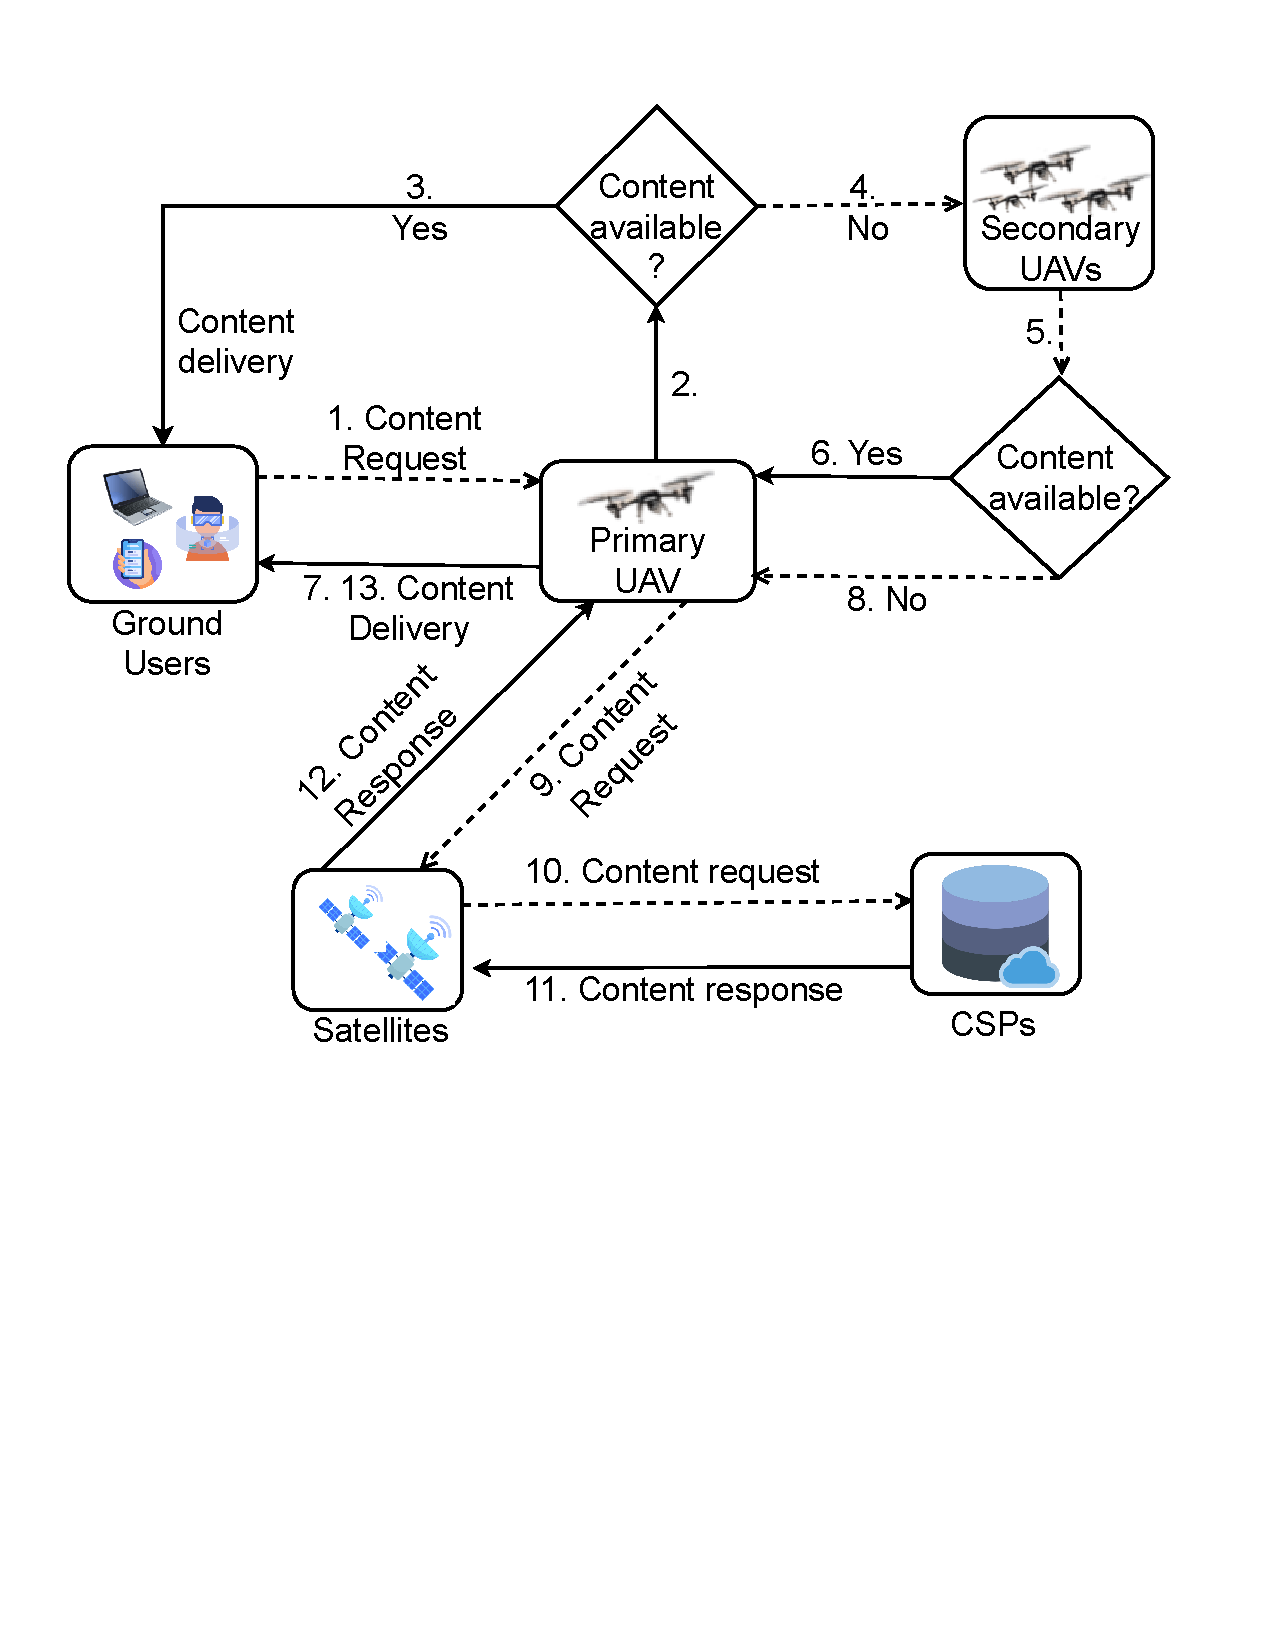
\includegraphics[width=\textwidth,trim=0.6cm 8.4cm 0.6cm 1.8cm, clip]{Diagrams/Flowchart.drawio (1).pdf}
        \caption{Workflow.}
        \label{fig:workflow}
    \end{minipage}
\end{figure*}
\section{Related Works}
Recent research has revealed that some well-known content is repeatedly requested by users, contributing to the most data traffic \cite{749260}. This puts substantial strain on the network, especially considering that UAVs serve ground users (GUs)by establishing a wireless backhaul connection to the content server. Because of its low capacity, this backhaul link frequently causes a bottleneck with the rapid development of data traffic, which eventually degrades the user experience. Popular content caching at the network edge has become a viable remedy for this. especially during peak traffic periods. Edge caching not only reduces the load on backhaul links but also improves responsiveness and quality of service. Moreover, caching can significantly extend UAV lifespan by enabling them to pre-store popular files and serve repeated requests locally, thereby minimizing the need for constant backhaul communication \cite{8982038, nguyen2023real, yang2023caching}.

Building on this foundation, several advanced strategies have been proposed to further optimize content delivery and resource usage. In \cite{10667821}, the authors address CSP cost minimization in 6G SAGIN via UAV caching and GU clustering. They adopt game theory and genetic algorithms to reduce latency and improve content placement efficiency under fixed power constraints. \cite{muller2016context} proposed a context-aware proactive content caching (m-CAC) scheme with service differentiation in wireless networks. By leveraging user context such as location and preferences, their approach reduces latency using a heuristic to solve the MINLP-based caching problem. A Q-learning-based collaborative caching algorithm tailored for vehicular clusters is proposed in \cite{bi2023collaborative}. This algorithm dynamically adapts to content popularity and user mobility, effectively reducing both latency and backhaul congestion. \cite{anokye2021deep} introduced a deep reinforcement learning (DRL)-based mobility-aware caching strategy, which also integrates UAV trajectory optimization using the DDPG algorithm. This joint optimization improves both content delivery efficiency and UAV movement planning. A DRL-based user association and caching framework in fog networks is presented in \cite{yan2020machine}. Utilizing Q-learning with experience relay, their method predicts content popularity and reduces content delivery delay. To enhance DRL training, \cite{wei2021deep} introduced a Quantum-Inspired Experience Replay (DRL-QiER) mechanism. By sampling experiences based on TD error and replay frequency, their method significantly improves learning efficiency compared to DRL-PER and DCRL. A DRL-based caching strategy for UAVs and user devices is developed in \cite{wang2021deep}. Their system pre-caches popular content in an end-to-end UAV-supported network, improving overall delivery efficiency. \cite{wu2020deep} presented a DRL-driven cache placement optimization algorithm for UAV networks. Their solution determines optimal caching strategies that reduce content delivery time and improve QoS. 
In another notable study, \cite{8374947} applied proactive caching directly at the GUs to address UAV endurance limitations. Their framework jointly optimizes caching policies, UAV path planning, and communication scheduling to enhance service delivery.
In \cite{huang2024joint}, authors proposed Fed-IDCCO, a federated deep reinforcement learning framework for joint data caching and computation offloading in UAV-assisted IoV. The approach minimizes task delay and maximizes cache hit ratio while preserving user privacy and improving training efficiency over baseline methods. Finally, \cite{liu2019deep} proposed a reinforcement learning framework that integrates content recommendation and proactive caching at the wireless edge to maximize the net profit of mobile network operators. By decomposing the large state-action optimization into two subproblems—a recommendation agent (enhancing user stickiness and revenue) and a pushing agent (minimizing transmission cost)—their double deep Q-network with dueling architecture achieved significant gains over baseline strategies.
% To address the existing problems in the literature, the cost minimization for Content Service Providers (CSP) in the SAGIN 6G model is proposed. Our work explores the cost-effectiveness of caching at UAVs within the SAGIN 6G.
% It promises to optimize network performance and reduce operational expenses for CSPs. Specifically, the contributions are summarized as follows:
% \begin{itemize}
 % \item This work investigates the downlink communication in a SAGIN 6G, comprising multiple Low Earth Orbit (LEO) satellites, UAVs, CSPs, and GUs.
    % \item We propose a novel satellite and cache assisted UAV communication model between GU and CSP.  
    % \item The proposed model, focused on minimizing the costs incurred by CSPs through UAV caching, and GU clustering while considering fixed Power Allocation (PA) at UAVs, satellite and CSP.
    % \item The problem is divided into two sub-problems: GU clustering, and cache placement. 
    % \item Game Theory (GT) is utilized to address the clustering problem, ensuring fairness among users. A Genetic Algorithm (GA) is used to determine the optimal cache placement among UAVs.

    % \item We address UAV clustering, cache placement, and power allocation. Using Game Theory (GT), we solve the clustering problem to ensure fairness between users. For optimal cache placement, we employ a genetic algorithm (GA) inspired by genetic mechanisms.
    % \item We use a genetic algorithm to optimize cache placement, enhancing efficiency and reducing costs in the 6G SAGINE network.
    % \item Our approach specifies the service provider cost function for network maintenance and resource allocation, using Game Theory and genetic algorithms to enhance network performance and reduce latency through efficient data storage and retrieval.
    % \item Satellite and UAV transmit power is estimated based on channel gain and request volume, avoiding complex optimization. This cost-effective method enhances satellite-terrestrial network performance, reducing CSP expenses.  
% The following section demonstrates the system model and problem formulation.
% % The proposed system model is discussed in the following: 
% The rest of the paper is organized as follows: Section II introduces the system model and the problem formulation. Section III proposes a solution. Section IV provides a performance evaluation to validate the efficacy of the proposed system. Finally, Section V presents conclusions and future research directions.
% This paper focuses on minimizing the costs incurred by CSPs through the use of UAV caching strategies. By strategically caching data on UAVs, the system aims to reduce the frequency of requests that need to traverse the entire network to reach the CSP. This approach not only reduces operational costs for CSPs but also enhances data delivery efficiency by leveraging the mobility and proximity of UAVs to users. The study explores how UAV caching can be a cost-effective solution in satellite-terrestrial networks, offering a promising approach to optimize network performance while reducing overall operational expenses for CSPs. We formulated a problem considering: UAV clustering, cache placement, and power allocation. Game theory (GT) is used to solve the clustering problem to ensure fairness between users. A genetic algorithm (GA), inspired by genetic mechanisms to tackle highly complex problems, is used to determine the optimal cache placement. For power allocation, we estimate the transmit power of satellites and UAVs considering channel gain and the number of requests, avoiding computationally intensive optimization algorithms.
% \begin{figure}[h] % 'h' means "here"
%     \centering
%     \includegraphics[width=0.8\textwidth]{SystemModel29may.png} % Replace with your filename
%     \caption{System architecture.}
%     \label{fig:example}
% \end{figure}
\section{System Model and Problem Formulation}
% In this work, we investigate the downlink communication architecture of a Satellite-UAV-Terrestrial Network (SUTN). The SUTN system model consists of several Low Earth Orbit (LEO) satellites, a fleet of UAVs, and a set of Ground Users (GUs).
%In this work, we examine the downlink communication setup of a Satellite-UAV-Terrestrial Network (SUTN), which comprises numerous Low Earth Orbit (LEO) satellites, a substantial fleet of Unmanned Aerial Vehicles (UAVs), and a massive quantity of Ground Users (GUs). In Fig. \ref{fig:model} show the configuration of the SUTN within a specified area. Fig. \ref{fig:model} illustrates the configuration of the SUTN within a specified area.
% Fig. \ref{fig:model} illustrates the layout of the SUTN within a designated geographical area, illustrating its configuration for clarity in the system model. We define the set of satellites as $\mathcal{S} = {\{1, 2, \ldots, S\}}$, Unmanned Aerial Vehicles (UAVs) as $\mathcal{U} = {\{1, 2, \ldots, U\}}$. These UAVs are equipped with some memory capabilities optimized for storage and efficient retrieval of frequently accessed files, thereby enhancing the system's ability to retain and access commonly utilized content. Additionally, there exist $K$ CSP represented by the set $C = \{{1, 2, \ldots, K\}}$, and $N$ users identified within the set $GU = {\{1, 2, \ldots, N\}}$. Furthermore, each GU is exclusively linked to a single UAV, whereas each UAV serves a cluster of GUs and has the capacity to serve $N_U$ GUs simultaneously. Here each UAV works as a flying relay station, equipped with single antenna serving its associated GUs under the following scenarios:
As illustrated in Fig. \ref{fig:model}, the proposed Space-Air-Ground Integrated Network (SAGIN) is designed to cover a designated geographical remote area. The system consists of several components, a set of satellites, denoted by \( \mathcal{S} = \{1, \ldots, s, \ldots, S\} \), a set of Unmanned Aerial Vehicles (UAVs), represented by \( \mathcal{U} = \{1, \ldots, u, \ldots, U\} \), and a Content Service Provider (CSP) denoted by $k$. Each UAV in the network is equipped with local memory to cache frequently accessed contents, enhancing service delivery and reducing latency. The content set \( \mathcal{F} = \{1, \ldots, f, \ldots, F\} \) is distributed across the CSPs, and there are \( N \) Ground Users (GUs) represented by the set \( \mathcal{GU} = \{1, \ldots, i, \ldots, N\} \). Each GU is associated with a single UAV, which serves as its direct communication node for content delivery. Multiple users can share the same UAV as their primary connection point. To improve efficiency and reliability in content distribution, UAVs are grouped into \(S\) clusters.

Within each cluster, UAVs can cooperate to fulfill user requests by sharing cached content. If a requested content is not available on a user's primary UAV, the system allows the request to be forwarded to one of the secondary UAVs—that is, other UAVs within the same cluster that are not directly associated with the user. These secondary UAVs support the content delivery process by acting as backup providers, enabling seamless transfer of data and ensuring that user demands are met even in the absence of local availability on the primary UAV.
The operation of the network proceeds in discrete updating periods, indexed by \( t \). During each period, every UAV simultaneously serves a fixed subset of ground users, denoted by \( M_u \), which remains unchanged throughout the duration of the period. UAVs are equipped with a single antenna and operate either as relay stations or direct service providers based on the availability of requested content.

The primary UAV initially determines if the content is locally cached when a user requests it. If  the content is transmitted directly to the user. However, if the content is not available on the primary UAV, the request is forwarded to another UAV within the same cluster that has the content cached. This inter-UAV communication ensures reliable delivery and minimizes delays by leveraging the cooperative structure of the network.If no UAV in the current UAV cluster has the content then, the primary UAV passes the content to the GU after receiving it from a CSP via satellite as a relay.
 %if another UAV in the current UAV cluster contains the file, it is relayed through the primary UAV to the GU. 
 
% Each UAV functions as a flying relay station, facilitated by a single antenna, to provide service to its associated GUs across three distinct cases as delineated below: We denote the set of satellites as $S = \{1, 2, \ldots, S\}$, UAVs as $U = \{1, 2, \ldots, U\}$ are equipped with some memory to store frequently accessed files, thereby facilitating the retention of commonly utilized content. $K$ content source providers with a set of $C = \{1, 2, \ldots, K\}$, and $N$ users with a set of $GU = \{1, 2, \ldots, N\}$. Furthermore, it is noteworthy that each GU is exclusively linked to a single UAV, whereas a single UAV has the capacity to serve multiple GUs simultaneously.Here are the transmission procedures based on the availability of the required file:

% \begin{itemize}
%     \item If the present UAV contains the required file within its cache, it directly transmits the file to the target GU. 
%     % If the primary UAV stores the required file in its cache, then the file will be directly transmitted to the target GU.
%     \item If the primary UAV lacks the necessary file in its cache but resides in the cache of another UAV within the same cluster, the file gets transmitted to the primary UAV and subsequently forwarded to the target GU.
%     % If the present UAV does not contain the required file within its cache, but is present in the cache of another UAV within the same cluster, the file will be transmitted to the primary UAV and then forwarded to the target GU.
%     \item If none of the UAVs in the same cluster as the primary UAV has the required file, one of the CSP will transmit the file to this UAV through one of the satellite, which will then forward it to the target GU.
% \end{itemize}
% A primary UAV $u$ for any $i^{th}$ GU is the one which connects directly to the $i^{th}$ GU. The secondary UAVs to GU $i$ are referred to other UAVs that are present in the same cluster of UAV $u$. 

% \subsection{UAV Mobility Model}

% The UAVs follows a fixed trajectory with a finite time period $T_v$. To simplify the description, we divide the flying duration $T_v$ into T equal time slots, where $dt$ represents the length of each time slot ($T_v$ = T$dt$). Assuming the UAVs' speed is $v$, it can move a maximum distance of $vdt$ in each time slot. Consequently, we can consider the distance between the satellites and the UAVs as well as the distance between the UAVs and users to remain constant during each time slot. For simplicity, we focus on the UAVs' stable flight process at a height $h$, excluding its take-off and landing phases \cite{9165228}. We are using $W_{u}(t): (x_{u}(t), y_{u}(t), h)$ for position of UAV $u$ at time slot $t$. The position of ground user $i$ is defined as $W_{i}(t): (x_{i}(t), y_{i}(t), 0)$, the position of user is randomly defined.
\subsection{Channel Model}
The channel between satellite and UAV is \cite{9755995}, \cite{10164260}:  
\begin{equation}
CG_{s, u}= [h_{s,u}]^T,\label{1}
\end{equation} 
where, $h_{s,u}$ $= \sqrt{g_{s,u}{ d_{s, u}^{-\alpha^{(1)}}}}$ is the satellite-to-UAV channel gain. $\alpha^{(1)}$ represents the path loss exponent between a satellite and a UAV, and $d_{s, u}$ indicates the distance between the $s^{\text{th}}$ satellite and the $u^{\text {th }}$ UAV and $g_{s,u}$ is the fading factor between satellite and UAV.  %Moreover,
% the expression $g_{s,u} \sim \text{SR}(\omega, \delta, \varepsilon)$ represents the SRF component, where $\omega$ denotes the average power of the direct signal, $\delta$ signifies half the average power of the scatter portion, and $\varepsilon$ represents the Nakagami-$m$ fading component.
% $g^{(s u)} \sim \operatorname{SR}\left(\omega, \delta, \varepsilon\right)$ corresponds to the SRF component with the average power of the direct signal $\omega$, half the average power of the scatter portion $\delta$, and the Nakagami-$m$ fading component $\varepsilon$.
Due to the page constraint we did not include the channel gain formula for CSP to satellite i.e., $CG_{k, s}$. However, it is considered based on Eq. \eqref{1} by changing the respective parameters\cite{10297374}.
% $2)$ CSP to Satellite Channel:
% The channel gain from the CSP to the satellite can be defined similarly to that from the satellite to the UAV, assuming a fixed UAV position.
% % The channel gain between CSP to satellite can be defined in same way as satellite to UAV considering  fixed UAV position.
% \begin{equation}
%     CG_{k, s}=g_{k,s}\sqrt{ d_{k, s}^{-\alpha^{(2)}}}
% \end{equation}
% where, $d_{k,s}$ is the distance between satellite and CSP, and $g_{k,s}$ is the fading factor between CSP and satellite. 
% The channel gain $CG_{u',u}$ from the secondary UAV $u'$ to the primary UAV $u$ is referred from \cite{9755995} and \cite{10164260}. 
% Similarly, the channel gain $CG_{u,i}$ between the $u^{th}$ UAV and the $i^{th}$ GU is obtained from \cite{7510820}.
%UAV to UAV Channel:In UAV-to-UAV communication, obstacles are notably scarce, leading to a prevalence of line-of-sight (LoS) components over non-line-of-sight (NLoS) components in UAV communications. As a result, the free-space path loss model is employed to describe UAV-to-UAV channels. 
% The channel gain from the secondary UAV $u'$ to the primary UAV $u$ \cite{9755995}, \cite{10164260} is expressed as:
% \begin{equation}
%     CG_{u',u}=g_{u',u}\sqrt{h_0d_{u',u}^{-\alpha^{(3)}}}
% \end{equation}
% where, $h_0$ signifies the power gain at the reference distance $d_0$, $d_{u',u}$ represents the distance between a primary UAV $u$ and a secondary UAV $u'$, $\alpha^{(3)}$ denotes the free-space path loss exponent, and $g_{u',u}$ describes the small-scale fading component characterized by a mean zero and unit variance.
% where $h_0$ denotes the power gain at the reference distance $d_0$, $d_{u',u}$ is the distance between a primary UAV $u$ and a secondary UAV $u'$, while $\alpha^{(3)}$ is the free-space path loss exponent, and $g_{u',u}$ represents the small-scale fading component with mean zero and unit variance.
% %UAV to GU Channel:
% The channel gain $CG_{u,i}$ between the $u^{th}$ UAV and the $i^{th}$ GU \cite{7510820}, \cite{9453853} is defined as:
% \begin{equation}
%     CG_{u,i}=g_{u,i}\left(\frac{4\pi f_cd_{u,i}}{c}\right)^{-\alpha^{(4)}/2}10^{-\frac{\eta^{LoS}P_{u,i}^{LoS}+\eta^{NLoS}P_{u,i}^{NLoS}}{20}}
% \end{equation}
% where, $f_c$ represents the carrier frequency, $d_{u,i}$ signifies the distance between a UAV and a GU, $c$ denotes the speed of light, $\alpha^{(4)}$ indicates the path loss exponent from a UAV to a GU, $g_{u,i}$ represents the small-scale fading component of the channel link between the UAV and GU, while $\eta^{LoS}$ and $\eta^{NLoS}$ correspondingly denote the weighted constant parameters of the Line-of-Sight (LoS) and Non-Line-of-Sight (NLoS) components. Moreover, $P^{NLos}_{u,i} = 1 - P^{Los}_{u,i}$ denotes the probability of NLoS, where $P^{Los}_{u,i}$ stands for the probability of the LoS component.
% where $f_c$ is the carrier frequency, $d_{u,i}$ is the distance between a UAV and a GU, $c$ is the speed pf light, $\alpha^{(4)}$ is the path loss exponenet from a UAV to a GU, $g_{u,i}$ is the small-scale fading component of the channel link between the UAV and GU, $\eta^{LoS}$ and $\eta^{NLoS}$ are respectively the weighted constant parameter of Los and NLoS components. $P^{NLos}_{u,i} = 1 - P^{Los}_{u,i}$ is the probability of NLoS, in which $P^{Los}_{u,i}$ is the probability of LoS component.

\subsection{Transmission Model}
% The data transmission rate between different entities in our model is given by:
The data rate between CSP and satellite is given as \cite{10297374}:
\begin{equation}
    R_{k,s} = B_1 \log_2\left(1 + \frac{CG_{k,s}P_{k}}{\sigma^2_s}\right), \label{Rks}
\end{equation}
where $B_1$ is the transmission bandwidth, $P_{k}$ is the transmit power of CSP, $CG_{k,s}$ is channel gain between CSP and satellite, $\sigma^2_s$ is the noise power.
The data rate between satellite $s$ and UAV $u$ ($R_{s,u}$)
% , primary UAV $u$ and GU $i$ ($R_{u,i}$) 
is considered based on Eq. \eqref{Rks} by changing the respective parameters \cite{10297374}.

\subsection{Caching Strategy and Content Popularity Prediction}

To efficiently manage content delivery in UAV-assisted networks, we define an association between UAVs and GUs as binary association matrix at time $t$, denoted by \textbf{$\mathcal{X}(t)$},  where each element \( x_{u,i}(t) \) represents the association  between UAV \( u \) and GU \( i \) as:
\begin{equation}
\small
x_{u,i}(t) = 
\begin{cases}
1, & \text{if the $u^{\text{th}}$ UAV is the primary UAV of GU $i$} \\
0, & \text{otherwise}
\end{cases}
\end{equation}
Here, $u$ denotes the primary UAV, and $u'$ represents a secondary UAV within the same cluster. For simplicity, the request packets used by GUs are considered negligible in size compared to the content files, and we assume error-free transmissions.
We assume that GU \( i \) requests the \( f^{\text{th}} \) content of size \( Z \) bits from its associated UAV \( u \). Satellites have access to all contents from CSP and transmit them to UAVs. Due to limited storage, each UAV can cache up to \( F' \) contents at a time, where \( F' \ll F \), and \( F \) is the total number of available contents.\\
We define the content popularity \( q_{i}^{f}(t) \) as the accumulated request behavior for content \( f \) by GU \( i \) in the update period \( t \). The actual content popularity \( Q^{f}_{u}(t) \)  of content $f$ for all GUs primarily served by UAV \( u \) is defined as follows \cite{9215049}:
\begin{equation}
Q^{f}_{u}(t) = \sum_{i \in \mathcal{GU}} x_{u,i}(t) q_{i}^{f}(t), \quad \forall f \in \mathcal{F}
\label{accumulate_request}
\end{equation}

It is necessary to forecast each content's overall popularity using the historical request data in order to implement proactive content caching during the updating period $t$. As a result, we indicate\(\hat{Q}^{f}_{u}(t)\) as the total predicted popularity of content $f$ for UAV $u$ which is the accumulated predicted request for a particular content $f$ for all GUs served by UAV $u$. Efficient content caching is a crucial aspect of modern wireless networks and edge computing systems.  However, a real challenge lies in accurately predicting the popularity of content and ranking it accordingly. To address this, we define the ranking function as \cite{9215049}:

\begin{equation} 
\text{rank}(\hat{Q}^{f}_{u}(t), \mathcal{F}) = \sum _ {f' \in \mathcal {F}} \boldsymbol {\mathbb{I}}\left (\hat{Q}^{f}_{u}(t) \leq \hat{Q}^{f'}_{u}(t) \right), 
\label{rank}
\end{equation} 
where $\mathbb{I}(\cdot)$ is the indicator function, which returns 1 if the condition inside holds true and 0 otherwise. This function counts how many other contents $f'$ in $\mathcal{F}$ have an estimated popularity equal to or greater than content $f$.
% $2)$ The data transmission rate between satellite and UAVs \cite{10297374} is defined as:
% \begin{equation}
%     R_{s,u} = B_2log_2\left(1 + \frac{CG_{s,u}^2P_{s}}{\sigma_u^2}\right)
% \end{equation}

% where $B_2$ is the transmission bandwidth, $P_{s}$ is the transmit power of the satellite, $CG_{s,u}$ is channel gain between satellite and UAV, $\sigma^2_u$ is the noise power.

% $3)$ The data transmission rate between secondary UAV and primary UAV \cite{10297374} is defined as:
% \begin{equation}
%     R_{u',u} = B_3log_2\left(1 + \frac{CG_{u',u}^2P_{u'}}{\sigma_u^2}\right)
% \end{equation}

% where $B_3$ is the transmission bandwidth, $P_{u'}$ is the transmit power of the secondary UAV, $CG_{u',u}$ is wireless channel gain between secondary UAV and primary UAV, $\sigma^2_u$ is the noise power.

% $4)$ The data transmission rate between Primary UAV and GU \cite{9874801} is defined as:
% \begin{equation}
%     R_{u,i} = B_4log_2\left(1 + \frac{CG_{u,i}^2P_{u}}{\sigma_i^2}\right)
% \end{equation}

% where $B_4$ is the transmission bandwidth, $P_{u}$ is the transmit power of the primary UAV, $CG_{u,i}$ is wireless channel gain between primary UAV and GU, $\sigma^2_i$ is the noise power. We neglect the cross-talk interference between different satellites in data transmission rate.


% % \subsection{Caching Scheme}
% % % We assume that a ground user (GU) \( i \) requests the \( i^{th} \) file from the primary UAV \( u \), with each file being \( Z \) bits in size. Throughout the paper, we have used the terms "file" and "user" interchangeably. Satellites have access to all these files from cloud service providers (CSPs) and transmit 


% % We assume that a GU $i$ requests $f^{th}$ content from primary UAV $u$ of $Z$ bits. 
% % % We assume that all GUs collectively request a maximum total of $F$ content files, each with a size of $Z$ bits. The files are indexed by the set $\mathcal{F} = \{{1, \ldots, F\}}$. 
% % Satellites have access to all these files from CSPs and transmit them to UAVs. However, each UAV is limited in its storage capacity and can only carry a maximum of $F'$ files ($F' \ll F$) at any given time.


% \subsection{Content Popularity Prediction}
% We define the content popularity \(q_{i,u}^{f}(t)\) as the accumulated request behaviors of content \(f\) for GU \(i\) for UAV $u$ in the update period \(t\).
% The actual total popularity \( Q^{f}_{u}(t) \) of content \( f \) for all GUs associated with UAV \( u \) during the update period \( t \) is calculated by considering only those GUs for which UAV \( u \) serves as the primary UAV. This is achieved by multiplying the individual popularity \( q_{i,u}^{f}(t) \) with the 

% as follows \cite{9215049}:

% \begin{equation}
% Q^{f}_{u}(t) = \sum_{i \in \mathcal{GU}(t)} x_{u,i}(t) \cdot q_{i,u}^{f}(t), \quad \forall f \in \mathcal{F}.
% \end{equation}


% For proactive content caching in the updating period t, the total popularity of each content needs to be predicted based on the historical request information. Denote \(\hat{Q}^{f}_{u}(t)\) as the total predicted popularity of content $f$ for UAV $u$. \\
% Efficient content caching is a crucial aspect of modern wireless networks and edge computing systems.  However, a real challenge lies in accurately predicting the popularity of content and ranking it accordingly.

% % The Least Frequently Used (LFU) caching strategy is widely adopted due to its ability to improve content availability and reduce latency. LFU prioritizes caching content based on its access frequency, where less frequently accessed content is replaced by more popular content.

% To address this, we define the ranking function as \cite{9215049}:

% \begin{equation} 
% \text{rank}(\hat{Q}^{f}_{u}(t), \mathcal{F}) = \sum _ {f' \in \mathcal {F}} \boldsymbol {\mathbb{I}}\left (\hat{Q}^{f}_{u}(t) \leq \hat{Q}^{f'}_{u}(t) \right), 
% \label{rank}
% \end{equation}
% where $\mathbb{I}(\cdot)$ is the indicator function, which returns 1 if the condition inside holds true and 0 otherwise. This function counts how many other contents $f'$ in $\mathcal{F}$ have an estimated popularity equal to or greater than content $f$.

\begin{table*}[t]
    \centering
    \caption{List of Notation}
    \label{tab:notation}
    \renewcommand{\arraystretch}{1.1} 
    \small % Reduce font size
    \resizebox{\textwidth}{!}{ 
    \begin{tabular}{|p{2cm}|p{6cm}|p{2cm}|p{6cm}|}
        \hline
        \textbf{Symbol} & \textbf{Meaning} & \textbf{Symbol} & \textbf{Meaning} \\
        \hline
        $\mathcal{S}$ & Set of Satellites & $\mathcal{U}$ & Set of UAVs \\ \hline
        $C$ & Set of Content Service Providers & $\mathcal{F}$ & Set of Content \\ \hline
        $\mathcal{GU}$ & Set of Ground Users & $s$ & Index of Satellite \\ \hline
        $u$ & Index of UAV & $k$ & Representation of a CSP \\ \hline
        $f$ & Index of Content & $i$ & Index of User \\ \hline
        $M_u$ & Maximum limit of users a UAV can serve & $CG_{i,j}$ & Channel Gain between $i$ and $j$ \\ \hline
        $R_{i,j}$ & Data rate between $i$ and $j$ & $\mathcal{U}_s$ & Cluster for UAVs of satellite $s$ \\ \hline
        $N$ & Total number of ground users & $F$ & Total number of contents/files \\ \hline
        $q^f_{i,u}(t)$ & Accumulated request count for content $f$ by GU $i$ for UAV $u$ in time slice $t$ & $Q^f_{u}(t)$ & Total actual popularity of content $f$ for all $\mathcal{GU}$ of UAV $u$ in time slice $t$ \\ \hline
        $\hat{Q}^f_{u}(t)$ & Predicted content popularity of $f$ for all $\mathcal{GU}$ of UAV $u$ in time slice $t$ & $L_u(t)$ & Transmission capacity of a UAV \\ \hline
        $\Gamma_{u,f}(t)$ & Binary variable denoting content $f$ is cached at UAV $u$ in time slice $t$ & $F'$ & Storage capacity of a UAV \\ \hline
        $ $ &  & $\mathcal{H}_u(t)$ & Cache hit for a UAV $u$ \\ \hline
        $\mathcal{R}(t)$ & System regret & $x_{u,i}$ & Binary variable for User-UAV association \\ \hline
        $\mathcal{X}$ & User-UAV Association Matrix & $d_{i,j}$ & Distance between $i$ and $j$ \\ \hline
        $\mathcal{F}_{{prev}}$ & Set of content cached at UAV $u$ at time $t$-$1$ & $C_{u}$ & Total cost that UAV has to pay for content retrieval from CSP via satellite \\ \hline
        $T_{i,j}$ & Latency between $i$ and $j$ & $N_{i,j}$ & Number of files transferred between $i$ and $j$ \\ \hline
        $D_{k,u}$ & Data transmitted between $k$ and $u$ & $C_{k,u}$ & Cost for communication between $k$ and $u$ \\ \hline
    \end{tabular}
    }
    \vspace{-3mm}
\end{table*}
The rank function is important because it helps decide which content should be saved in the cache. If the rank is low (closer to 1), it means the content is popular and should be stored. If the rank is high, it means the content is less popular and might not be kept in the cache. By leveraging this ranking mechanism, the caching system is dynamically updating stored content based on real-time popularity trends, thereby optimizing cache efficiency and network performance.

% \textbf{Theorem 1: Content placement vector based on predicted content popularity } 
% \\

We define the cache placement vector for a particular UAV \( u \) in updating period \( t \), denoted as $\boldsymbol{\Gamma_{u}(t)}$, as the binary vector representing the cached state of content \( f \) in updating period \( t \), determined based on the predicted total popularity while satisfying the maximum cache capability constraint \( F' \) and the transmission capacity constraint $\boldsymbol{L_u(t)}$. Here, the transmission capacity constraint is the maximum number of contents that can be retrieved from the CSP depending on available battery and power resources of a UAV. Mathematically, $\boldsymbol{\Gamma_{u}(t)}$ is defined as ,
\(
    \boldsymbol{\Gamma_{u}(t)} = \left\{\Gamma_{u,f}(t) \mid f \in \mathcal{F} \right\},  
\) where \( \Gamma_{u,f}(t) \) is a binary indicator denoting whether the \( f \)-th content is stored in the cache of UAV \( u \), with \( \Gamma_{u,f}(t) \in \{0, 1\} \). Here, a value of 1 means the content is stored in the cache of UAV \( u \), while 0 means the content is not stored in that UAV. Each UAV \( u \) has a cache storage limit, expressed as: 
\begin{equation}
    \sum_{f \in \mathcal{F}}  \Gamma_{u,f}(t)\leq F'.
\end{equation} 
However, without considering the transmission constraint, the ideal cached content vector \( \boldsymbol{\tilde{\Gamma}}_u(t) \)
depends only on the predicted popularity ranking, defined by 
\[
    \tilde{\Gamma}_u(t) \triangleq \left\{   \tilde{\Gamma}_{u,f}(t) = \mathbb{I} \left( \text{rank}(\hat{Q}^{f}_{u}(t), \mathcal{F}) \leq F' \right) \mid f \in \mathcal{F} \right\}.
\] \\
We define the cache update load as the number of contents that must be updated in the cache, which is given as:
\begin{equation}
    \Delta \Gamma_{u}(t) = \sum_{f \in \mathcal{F}} \left| \boldsymbol{\tilde{\Gamma}_{u,f}(t)} - \boldsymbol{\Gamma_{u,f}(t-1)} \right|,
\end{equation} Then, the updated cache placement vector \( \boldsymbol{\Gamma_{u}(t)} \) is determined as follows:

\begin{itemize}
    \item {If \( L_u(t) \geq \Delta \Gamma_{u}(t) \)}: The UAV has sufficient transmission resources to retrieve all required files from the CSP via satellite, then:
    \(
        \boldsymbol{\Gamma_{u}(t)} = \boldsymbol{\tilde{\Gamma}_u(t)},
    \)
    meaning that the files with the top \( F' \) predicted popularity ranking will be cached.

    \item {If \( L_u(t) < \Delta\Gamma_{u}(t) \)}: The UAV can retrieve at most \( L_u(t) \) files from the CSP, then:
\(
    \boldsymbol{\Gamma_{u}(t)} = \boldsymbol{\Gamma_{u,1}(t)} + \boldsymbol{\Gamma_{u,2}(t)},
\)
in which :
\begin{align*}
    \Gamma_{u,1,f}(t) &= \mathbb{I} \left( \text{rank} \left(\hat{Q}^{f}_{u}(t), \mathcal{F}_{{prev}} \right) \leq F' - L_u(t) \right), \\
    \Gamma_{u,2,f}(t) &= \mathbb{I} \left( \text{rank} \left(\hat{Q}^{f}_{u}(t), \mathcal{F} \setminus \mathcal{F}_{{prev}} \right) \leq L_u(t) \right),
\end{align*} where $\mathcal{F}_{{prev}} = \{ f \in \mathcal{F} \ | \ \boldsymbol{\Gamma_{u,f}(t-1)} = 1\}$ denotes the set of contents cached at previous time slot. Here, \( \boldsymbol{\Gamma_{u,1}(t)} \) represents the files retained from the previous cache at UAV \( u \). Meanwhile, \( \boldsymbol{\Gamma_{u,2}(t)} \) represents the \( L_u(t) \) files retrieved from the CSP at time \( t \).
\end{itemize}
Then, the network fulfills user requests for content in \( \mathcal{F} \) via the following three phases:

\begin{itemize} 
    \item \textbf{Phase 1: Direct Cache Delivery} \\
    For content \( f  \in \mathcal {F} \) such that \( \Gamma_{u,f}(t) = 1 \), the requested content is proactively cached at UAV \( u \) and can be directly delivered to the user.

    \item \textbf{Phase 2: Cluster-Assisted Delivery} \\
   For content \( f \in \mathcal{F} \) such that \( \Gamma_{u,f}(t) = 0 \), but \( \Gamma_{u',f}(t) = 1 \) for any UAV \( u' \) that belongs to the same cluster as UAV \( u \), the requested content is first retrieved from UAV \( u' \) and then delivered to the user through UAV \( u \).


    \item \textbf{Phase 3: Content Retrieval from CSP via Satellite} \\
    For content \( f \in \mathcal{F} \) such that \( \Gamma_{u,f}(t) = 0 \) and \( \Gamma_{u',f}(t) = 0 \) for all UAVs \( u' \) in the same cluster — where a cluster is defined as a group of UAVs that are jointly served by a common satellite and are responsible for delivering content to their associated ground users — the requested content must be retrieved from the CSP via satellite transmission.

\end{itemize}
Given the cache placement vector \(\boldsymbol{\Gamma_{u}(t)}\), the total cache hit ratio of these cached contents, denoted as \( \mathcal{H}_u(t)\), is calculated as: 
\begin{align}
    \mathcal{H}_u(t) = \frac{ {\sum\limits_{f \in \mathcal{F}} \Big( \Gamma_{u,f}(t) + (1 - \Gamma_{u,f}(t)) \max\limits_{u' \in \mathcal{U}_{s}} \Gamma_{u',f}(t) \Big) \hat{Q}^f_{u}(t)}}{\sum\limits_{f' \in \mathcal{F}} \hat{Q}^{f'}_{u}(t)}. \label{cachehit}
\end{align}

% \begin{align}
%     \mathcal{H}_u(t) = 
%     &\frac{
%         \sum\limits_{u \in \mathcal{U}_s} x_{u,i} 
%         \Bigg( 
%             \sum\limits_{f \in \mathcal{F}}  
%             \Gamma_{u,f}(t) Q^f_{u}(t)
%         \Bigg) 
%     }{
%         \sum\limits_{f' \in \mathcal{F}} Q^{f'}_{u}(t)
%     } \notag \\[8pt]
%     &+ 
%     \frac{
%         \sum\limits_{u \in \mathcal{U}_s} x_{u,i} 
%         \Bigg( 
%             \sum\limits_{f \in \mathcal{F}}  
%             (1 - \Gamma_{u,f}(t)) \max\limits_{u' \in \mathcal{U_s}} \Gamma_{u',f}(t) Q^f_{u}(t)
%         \Bigg) 
%     }{
%         \sum\limits_{f' \in \mathcal{F}} Q^{f'}_{u}(t)
%     }.
%     \label{cachehit}
% \end{align}


%  Now our goal is to design the popularity prediction scheme for minimizing the system regret, which is defined as the difference between the \textit{total cache hit ratio} (\ref{cachehit}) and the \textit{maximal total cache hit ratio}. Before formulating the system regret, we first discuss the maximal total cache hit ratio, which is achieved by caching the contents according to the actual popularity ranking. Therefore, we denote \(\text{rank}(Q^f_{u}(t), \mathcal {F})\) as the actual popularity ranking of content \(f\) in updating period \(t\), which is calculated as similar to eq. (\ref{rank}) as :
 
% \begin{equation}
% \text{rank}(Q^f_{u}(t), \mathcal{F}) = \sum_{f' \in  \mathcal{F}} \mathbb{I}(Q^f_{u}(t) \leq Q^{f'}_{u}(t))
% \label{cache_hit}
% \end{equation}
% Then we have the following theorem of the maximal-hit-ratio file set under the constraints on the cache capacity $F'$ and the transmission capacity $L_u(t)$.

% \textbf{Theorem 2: Maximal-hit-ratio Content placement vector based on Actual content popularity} \\
% The maximal-hit-ratio content vector in updating period \(t\), denoted as $\boldsymbol{\xi_u(t)}$ , is defined as the binary vector of files which ought to be cached in updating period \(t\) according to the actual total popularity under the constraints on the cache capability $F'$ and the transmission capacity $L_u(t)$. Without considering the transmission constraint, the ideal maximal-hit-ratio content vector $\tilde{\xi_u}(t)$
% depends only on the actual popularity ranking, that is, \[     \boldsymbol{\tilde{\xi}_u(t)} \triangleq \left\{   \tilde{\xi}_{u,f}(t) = \mathbb{I} \left( \text{rank}({Q}^{f}_{u}(t), \mathcal{F}) \leq F' \right) \mid f \in \mathcal{F} \right\}. \] \\
% Define the cache update load as:
% \begin{equation}
%     \Delta {\xi_{u}(t)} = \sum_{f \in \mathcal{F}} \left| \tilde{\xi}_{u,f}(t) - {\Gamma_{u,f}(t-1)} \right|,
% \end{equation}
% which represents the number of files that must be updated in the cache. The maximal-hit-ratio content placement vector \( \boldsymbol{\xi_u(t)} \) is determined as follows:

% \begin{itemize}
%     \item \textbf{If \( L_u(t) \geq \Delta \xi_{u}(t) \)}: The UAV has sufficient transmission resources to retrieve all required files from the CSP via satellite, then:
%     \(
%         \boldsymbol{\xi_{u}(t)} = \boldsymbol{\tilde{\xi}_u(t)},
%     \)
%     meaning that the files with the top \( F' \) predicted popularity ranking will be cached.

%     \item \textbf{If \( L_u(t) < \Delta\xi_{u}(t) \)}: The UAV can retrieve at most \( L_u(t) \) files from the CSP, then:
% \(
%     \boldsymbol{\xi_{u}(t)} = \boldsymbol{\xi_{u,1}(t)} + \boldsymbol{\xi_{u,2}(t)},
% \) where:
% \begin{align*}
%     \xi_{u,1,f}(t) &= \mathbb{I} \left( \text{rank} \left({Q}^{f}_{u}(t), \mathcal{F}_{{prev}} \right) \leq F' - L_u(t) \right), \\
%     \xi_{u,2,f}(t) &= \mathbb{I} \left( \text{rank} \left({Q}^{f}_{u}(t), \mathcal{F} \setminus \mathcal{F}_{{prev}} \right) \leq L_u(t) \right),
% \end{align*} in which $\mathcal{F}_{{prev}} = \{ f \in \mathcal{F} \ | \ \Gamma_{u,f}(t-1) = 1\}$ denotes the set of contents cached at previous time slot. Here, \( \boldsymbol{\xi_{u,1}(t)} \) represents the files retained from the previous cache at UAV \( u \). Meanwhile, \( \boldsymbol{\xi_{u,2}(t)} \) represents the \( L_u(t) \) files retrieved from the CSP at time \( t \) that indicates which file is ought to be retrieved from the CSP based on actual popularity value of content.
% \end{itemize} 
% Accordingly, the maximal total cache hit ratio of the cached files, denoted as \(\mathcal{H}_{u}^{\text{max}}(t)\), can be calculated as:

% \begin{align}
%     \mathcal{H}_u^{\text{max}}(t) = \frac{ {\sum\limits_{f \in \mathcal{F}} \Big( \xi_{u,f}(t) + (1 - \xi_{u,f}(t)) \max\limits_{u' \in \mathcal{U}_{s}} \xi_{u',f}(t) \Big) Q^f_{u}(t)}}{\sum\limits_{f' \in \mathcal{F}} Q^{f'}_{u}(t)}. \label{maxcachehit}
% \end{align}
% % \begin{align}
% %     \mathcal{H}^{\max}_u(t) =
% %     &\frac{
% %         \sum\limits_{u \in \mathcal{U}_s} x_{u,i} 
% %         \Bigg( 
% %             \sum\limits_{f \in \mathcal{F}}  
% %             \xi_{u,f}(t)
% %         \Bigg) {Q}^{f}_{u}(t)
% %     }{
% %         \sum\limits_{f' \in \mathcal{F}} {Q}^{f'}_{u}(t)
% %     } \notag \\[8pt]
% %     &+ 
% %     \frac{
% %         \sum\limits_{u \in \mathcal{U}_s} x_{u,i} 
% %         \Bigg( 
% %             \sum\limits_{f \in \mathcal{F}}  
% %             (1 - \xi_{u,f}(t))\max\limits_{u' \in \mathcal{U_s}} \xi_{u',f}(t) 
% %         \Bigg) {Q}^{f}_{u}(t)
% %     }{
% %         \sum\limits_{f' \in \mathcal{F}} {Q}^{f'}_{u}(t)
% %     }.
% % \end{align}
% Note that \(\mathcal {H}_u(t) \leq \mathcal {H}_u{^\text{max}}(t)\), and \(\mathcal{H}_u^{\text{max}}(t)\) is always achieved only under the condition that \(\boldsymbol{\Gamma_{u}(t)} = \boldsymbol{\xi_u(t)}\), that is, accurate prediction of popularity ranking. However, since prediction errors are inevitable with any approach, the total predicted popularity is often inaccurate. These inaccuracies lead to errors in the predicted popularity ranking, which in turn negatively impact caching performance. To measure the influence of popularity prediction on caching performance, we formally define the system regret as follows.

To evaluate the performance of the system, we define system regret as the cache miss in updating period \(t\), denoted as \(\mathcal{R}(t)\), which is the loss of the total cache hit ratio from cache vectors 
% between the vector \(\boldsymbol{\xi_u(t)}\) of files that ought to be cached and the vector
\(\boldsymbol{\Gamma_{u}(t)}\) of contents that are cached for each UAV. For a single UAV \( u \), the regret is given by:
\begin{equation}
    \mathcal{R}_u(t) = 1 - \mathcal{H}_u(t).
\end{equation}
Extending this to all UAVs in the system, the total system regret is expressed as:
\begin{equation}
    \boldsymbol{\mathcal{R}(t)} = \sum\limits_{u \in \mathcal{U}} \mathcal{R}_u(t).
    \label{systemregretall}
\end{equation}
Now, when a user request for content results in a cache miss, i.e., the requested file is unavailable at both the primary UAV and its neighboring UAVs within the same cluster, the content must be fetched directly from 
CSP via satellite. This retrieval involves data transmission over satellite and backhaul links, thereby incurring both latency and communication cost. To comprehensively evaluate system performance under such cache miss scenarios, we analyze the total latency experienced during CSP retrieval and quantify the associated communication cost required to cache the missing content at the UAV.

% The expectation of the system regret is then:
% \begin{equation}
%     \mathbb{E}[\mathcal{R}(t)] = \sum\limits_{u \in \mathcal{U}} \mathbb{E}[\mathcal{R}_u(t)]
%     \label{expectation_regret}
% \end{equation},
% where \(\mathbb{E}(\cdot)\) denotes the expectation with respect to the probability measure of the system regret \(\mathcal{R}_u(t)\), induced by the unknown actual total popularity.
\subsection{Latency and Communication Cost}

 If the required content $f$ is not present in the cache of either the primary UAV $u$ or the secondary UAV $u'$, then the content has to be bought from CSP. The latency for bringing that content from CSP via satellite as a relay is formulated as \cite{10667821}:
 
\begin{equation} \label{12}
        T_{k,u} = T_{k,s}+ T_{s,u},
\end{equation}    
where, 
\begin{equation} \label{14}
        T_{k,s} = \frac{2d_{k,s}}{c}  + \frac{N_{k,s}Z}{R_{k,s}}.
\end{equation}

\begin{equation} \label{13}
        T_{s,u} = \frac{2d_{s,u}}{c}  + \frac{N_{s,u}Z}{R_{s,u}},
\end{equation}
By Eqs. \eqref{12}, \eqref{14}, and \eqref{13} we write $T_{k,u}$ as \cite{10667821}:
\begin{equation}
        T_{k, u} = \frac{2(d_{k,s}+d_{s,u})}{c} + \frac{N_{s,u}Z}{R_{s,u}} + \frac{N_{k,s}Z}{R_{k,s}},
\end{equation}
where, $N_{s,u}$, $N_{k,s}$ represent the number of files transferred between satellite $s$ and UAV $u$, and CSP $k$ and satellite $s$ respectively. When data is transmitted from CSP to UAV , the cost borne for the communication via backhaul(satellite) is given by \cite{10667821}:
\begin{equation}
    C_{k,u} =p^k D_{k,u},
\end{equation}
where, $p^k$ is the cost per bit for data transfer and $D_{k,u}$ is the size of data to be transferred from CSP to UAV, defined as \cite{10667821},
\begin{equation}
    D_{k,u} = R_{s,u}  T_{s,u} + R_{k,s}  T_{k,s}.
\end{equation}
Now, for completely caching the missing contents  on UAV $u$, the total communication cost is formulated as:
\begin{equation}
    C_u(t) =  \sum_{f \in \mathcal{\tilde{F}}} \left( (1 -  \Gamma_{u,f}(t))(1 - \max_{u' \in \mathcal{U}_s} \Gamma_{u',f}(t)) C_{k,u} \right)
\end{equation}
where  $\mathcal{\tilde{F}}$ is the set of contents which are to be fetched from CSP via satellite in case of cache miss from the cluster, which is defined as  $\mathcal{\tilde{F}} = \{ f \in \mathcal{F} \ | \ \text{rank} \left({Q}^{f}_{u}(t), \mathcal{F} \setminus \mathcal{F}_{{prev}} \right) \leq L_u(t) \}$
% $\mathcal{\tilde{F}} = \{f \ | \ \text{rank}(Q^f_{u}(t),\mathcal{{F}}) \leq F'\}$.
% $\mathcal{\tilde{F}} = \{f \ | \ \text{rank} \left({Q}^{f}_{u}(t), \overline{\Gamma_u(t-1)} \right) \leq L_u(t)\}
% $
. Extending this to all UAVs in the system, the total system cost is expressed as:
\begin{equation}
    \boldsymbol{\mathcal{C}(t)} = \sum\limits_{u \in \mathcal{U}} \mathcal{C}_u(t).
    \label{costall}
\end{equation}
% \begin{equation}
%     C^{k} = \sum_{u \in U} \sum_{i \in GU}(C^k_{u,i} + C^k_{u',u,i} + C^k_{k,u,i} + Y\Gamma^{(u)}_{i})
% \end{equation}
% where, $\sum_{u \in \mathcal{U}} \sum_{i \in {GU}}\Gamma^{(u)}_{i}$ is the no. of files cached, and $Y$ is the cost of caching one file.
% Additionally, in our simulation, we consider $\boldsymbol{P}_{s}, \boldsymbol{P}_{u},$ , $\boldsymbol{P}_{k}$ and $\mathcal{X}$  to be fixed.
% \textbf{Joint Problem : Content Placement Problem} \\
In practice, it is crucial to create a balance between minimizing the cache miss rate and reducing the communication cost incurred during content retrieval from the CSP via satellite backhaul links. To address the tradeoff between the cache hit ratio and communication cost for content retrieval in case of cache miss, we formulate a joint optimization framework that aims to minimize the overall system cost by effectively managing content placement decisions. The objective is to reduce the system regret incurred due to suboptimal cache hits while simultaneously minimizing the retrieval cost from CSP in the event of cache misses. The optimization problem is expressed as follows: 
\begin{equation}
    \text{P$1$}:\quad \min_{\boldsymbol{\Gamma(t)}} \boldsymbol{\mathcal{R}(t)} +\boldsymbol{{C}^{\text{norm}}(t)} \label{systemregret}
\end{equation}
subject to the following constraints:
\begin{align}
    & \quad \Gamma_{u,f}(t) \in \{0,1\}, \quad \quad\forall u\in \mathcal{U}, f \in \mathcal{F}, \tag{\ref{systemregret}a} \label{systemregretC1} \\
    & \quad \sum_{f \in \mathcal{F}} \Gamma_{u,f}(t) \leq F', \quad \forall u \in \mathcal{U}, \tag{\ref{systemregret}b} \label{systemregretC2} \\
    & \quad \Delta{\Gamma_{u}(t)} \leq L_u(t) , \quad \forall u \in \mathcal{U}   \tag{\ref{systemregret}c} \label{systemregretC3} 
    % & \quad \sum_{f \in \mathcal{F}} \xi_{u,f}(t) \leq F', \quad \forall u \in \mathcal{U}. \tag{\ref{systemregret}d} \label{systemregretC4}
\end{align}, where $\boldsymbol{{C}^{\text{norm}}(t)}$ is the normalized cost. To ensure consistent scaling across different metrics, we normalize the cost using min-max normalization, computed as \(
\boldsymbol{{C}^{\text{norm}}(t)} = \frac{\boldsymbol{C}(t) - \min \boldsymbol{C}(t)}{\max \boldsymbol{C}(t) - \min \boldsymbol{C}(t)}.
\label{eq:minmax_cost}
\) This normalization is necessary because the system regret (i.e., cache miss) for each UAV is naturally bounded between 0 and 1, while the cost values can span a wider numerical range. By applying Min-Max normalization, we scale the cost into the same range $[0, 1]$ for balanced optimization.




\section{Proposed Solution}
% \begin{figure*}[h]
%     \centering
%     \begin{minipage}{0.45\textwidth}
%         \centering
%         \hspace*{-1.2cm} % Shift the image to the left
%     \includegraphics[page=2,width=\textwidth,trim=0cm 10cm 0cm 4cm, clip]{UAV_workflow.drawio (3).pdf}
%         \caption{UAV workflow}
%         \label{fig:uAV_workflow_model}
%     \end{minipage}
%     % \hfill
%     \begin{minipage}{0.45\textwidth}
%         \centering
%         \includegraphics[width=\textwidth,trim = 0.6cm 12cm 0.6cm 1.5cm]{ddqn_workflow.drawio.pdf}
%         \caption{Heuristic DDQN Workflow}
%         \label{fig:DDQN_workflow}
%     \end{minipage}
% \end{figure*}

\begin{figure*}
    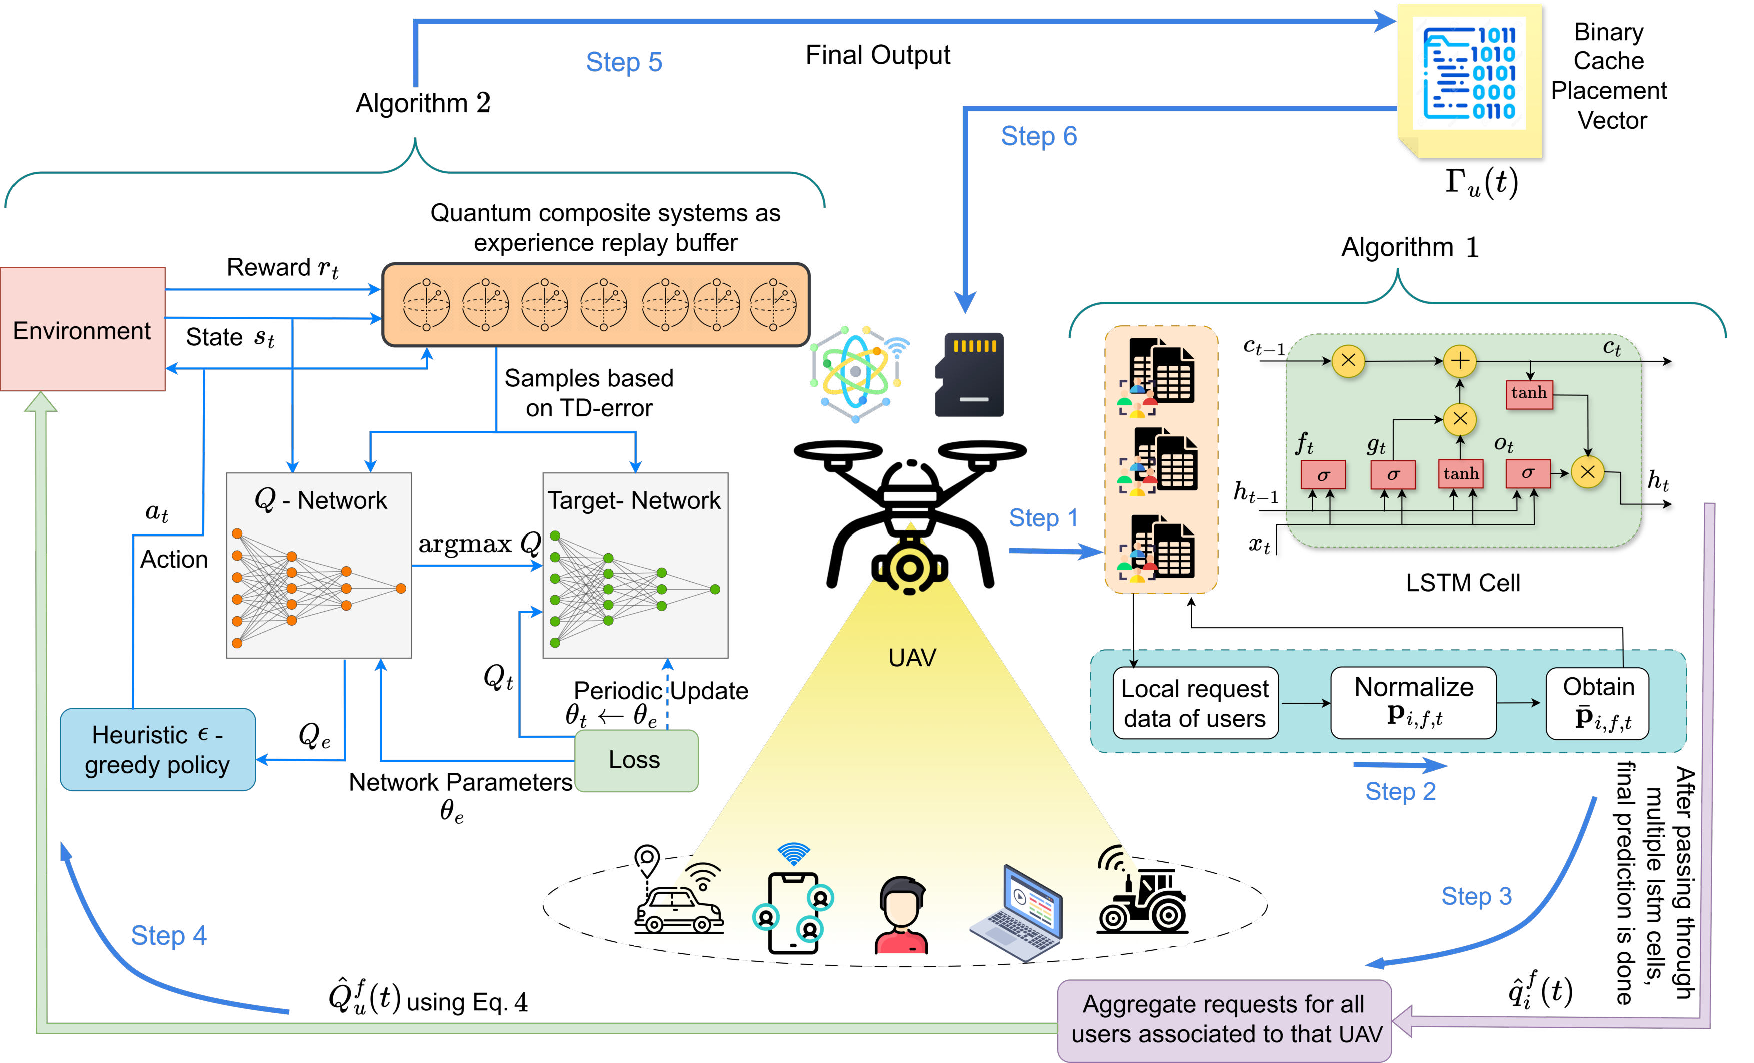
\includegraphics[width=\textwidth]{Diagrams/UAV_workflow (2) (1).pdf}
        \caption{UAV sequential workflow}
        \label{fig:uav_sequential_workflow}
\end{figure*}

To address the above joint regret and cost minimization problem, we propose an integrated prediction–decision framework. This section is divided into two parts: (i) an LSTM-based content popularity prediction approach, and (ii) a Heuristic Deep Reinforcement Learning (DRL) inspired framework for cache placement.


\subsection{Long Short Term Memory (LSTM)}

The Long Short-Term Memory (LSTM) network \cite{hochreiter1997long}, a prominent type of recurrent neural network (RNN), is extensively employed for modeling sequential data. It has demonstrated remarkable performance in a variety of tasks, including speech recognition \cite{graves2014towards}, machine translation \cite{sutskever2014sequence}, syntactic parsing \cite{vinyals2015grammar}, and image captioning \cite{xu2015show}. Owing to its effectiveness in capturing temporal dependencies, the LSTM architecture is particularly well-suited for our content request prediction task. In the following subsection, we briefly describe the structure of the LSTM network.

The input gate $g_t$, forget gate $f_t$, and output gate $o_t$ are built as sigmoid units to selectively pass information, and each of the memory blocks that make up the LSTM network contains a memory cell that is controlled by these three gates. The input gate $g_t$ decides how much new information is supplied to create the updated cell state $c_t$, while the forget gate $f_t$ regulates how much of the prior cell state $c_{t-1}$ is kept. Through recurrent connections, the cell output $h_t$ and $c_t$ are transmitted to the following time step after being modulated by the output gate $o_t$. The LSTM generates an output $h_t$ and changes its cell state $c_t$ at each time $t$. This output is used to forecast the content request $\hat{q}^f_i(t)$, based on the previous state $c_{t-1}$, previous output $h_{t-1}$, and the current input $x_t$ (i.e., the normalized content request $\bar{q}^f_i(t-1)$). Given the limited number of user requests, which makes individual demand hard to forecast accurately, we instead predict the aggregate number of requests for each content item per time slot, where $Q^f_u(t)$ denotes the total \textbf{actual popularity} of content $f$ across all users served by UAV $u$.

Let \( {\textbf{p}}_{i,f,t} \in \mathbb{R}^\rho \) represent a \( \rho \)-dimensional integrated feature vector that captures the historical request behavior of GU \( i \) for content \( f \) at time slot \( t \). This vector is defined as:
\(
{\textbf{p}}_{i,f,t} = [q^f_{i}(t - \rho), q^f_{i}(t - \rho + 1), \dots, q^f_{i}(t - 1)],
\)
where \( \rho \) denotes the number of preceding time slots considered. Hence, \( \textbf{p}_{i,f,t} \) aggregates the past \( \rho \) content requests made by GU \( i \) for content \( f \).

To mitigate the influence of varying magnitudes in request values, we normalize this feature vector. Let \( \bar{\textbf{p}}_{i,f,t} \) denote the normalized version of \( \textbf{p}_{i,f,t} \), given by:
\(
\bar{\textbf{p}}_{i,f,t} = \left[ \bar{q}^f_{i}(t - \rho),\bar{q}^f_{i}(t - \rho+1), \dots, \bar{q}^f_{i}(t-1) \right],
\)
where each normalized request is computed as:
\(
\bar{q}^f_{i}(t - \rho) = \frac{q^f_{i}(t - \rho)}{\max \{ \textbf{p}_{i,f,t} \}},
\)
and \( \max \{ \textbf{p}_{i,f,t} \} \) denotes the maximum entry within the feature vector \( \textbf{p}_{i,f,t} \).\\
For each UAV \( u \), we employ an LSTM network consisting of three hidden LSTM layers, along with an input and an output layer, to predict future content popularity. Let \( \mathcal{L}_u(\cdot) \) be the output function of this LSTM network, parameterized by weights \( \theta_u \). At the start of time slot \( t \), the normalized input vectors \( \bar{\textbf{p}}_{i,f,t} \) are generated using the aforementioned procedure. The predicted request (popularity) of content \( f \) by GU \( i \) at time \( t \), denoted \( \hat{q}^f_{i}(t) \), is then obtained as follows~\cite{9234632}:
\begin{equation}
    \hat{q}^f_{i}(t) = \max \{\bar{\textbf{p}}_{i,f,t}\} \cdot \mathcal{L}_u(\bar{\textbf{p}}_{i,f,t}  | \theta_u).
    \label{lstm_predict}
\end{equation} \\
The LSTM parameters \( \theta_u \) are trained by minimizing the squared loss between the predicted value \( \hat{q}^f_{i}(t) \) and the actual number of requests \( q^f_{i}(t) \), where the target is also normalized. The corresponding loss function is defined as~\cite{9234632}:
\begin{equation}
    \text{Loss}(\theta_u) = \left( \mathcal{L}_u(\bar{\textbf{p}}_{u,t,f}  | \theta_u) - \frac{q^f_{i}(t)}{\max\{{\textbf{p}}_{u,f,t} \}} \right)^2.
    \label{lstmloss}
\end{equation}\\
After computing the predicted popularity \( \hat{q}^f_{i}(t) \) for each GU \( i \) associated with UAV \( u \), the total predicted popularity of content \( f \) across all connected users at time slot \( t \), denoted as \( \hat{Q}_{u}^{f}(t) \), is obtained using Eq.~\ref{accumulate_request}.

% Let \( {\textbf{p}}_{i,f,t} \in \mathbb{R}^\rho \) denote a \( \rho \)-dimensional integrated feature vector of content \( f \) and GU $i$ at time slot \( t \), which is defined as, 
% \(
% {\textbf{p}}_{i,f,t} = [q^f_{i}(t - \rho), q^f_{i}(t - \rho + 1), \dots, q^f_{i}(t - 1)]
% \)
% where \( \rho \) is the number of historical time slots used. The feature vector \( \textbf{p}_{i,f,t} \) contains the historical requests of content \( f \) by GU $i$ during the previous time slots, where \( \rho \) is a design parameter. In order to eliminate the difference in the absolute value of the request number, let \( {\bar{\textbf{p}}_{i,f,t}} = \big[ \bar{q}^f_{i}(t - \rho),\bar{q}^f_{i}(t - \rho+1), \dots, \bar{q}^f_{i}(t-1) \big] \) denote the normalized feature vector, where 
% \(
% \bar{q}^f_{i}(t - \rho) = \frac{q^f_{i}(t - \rho)}{\max \{ \textbf{p}_{i,f,t} \} }
% \) and \(\max \{ \textbf{p}_{i,f,t} \}\) presents the maximum value of all the elements in $\textbf{p}_{i,f,t}$.

% The similarity between two feature vectors is measured by the Euclidean distance between the corresponding normalized vectors. To begin with i.e. (\( t = \rho + 1 \)), we adopt the method in \cite{arthur2006k} to randomly select \( C \) points from the \( F \) feature vectors \( \{  {\bar{\textbf{p}}_{\rho+1,1}}, {\bar{\textbf{p}}_{\rho+1,2}}, \dots , \bar{\textbf{p}}_{\rho+1,{F}}\}\), denoted as \( \{  {{\textbf{p}}_{1}^c}, {{\textbf{p}}_{2}^c}, \dots , {\textbf{p}}_C^c\}\) , to be the initial cluster center. Specifically,  we first randomly select one of the $\mathcal{F}$ feature vector as the
% first initial cluster center ${\textbf{p}}_{1}^c$. We then select each subsequent
% initial cluster center at random with a probability proportional
% to the distance from itself to the closest center that has been
% already chosen. 
% \\ At the beginning of each time slot \( t \geq \rho + 1\), we determine the cluster membership of the newly-observed feature vectors ${\bar{\textbf{p}}_{t,f}}$ , $\forall f \in \mathcal{F} $, according to the minimum Euclidean distance criterion . More Specifically \cite{9234632}: 

% \begin{equation}
%     I(\bar{\textbf{p}}_{t,f}) = \arg \min_{j \in 1,2,\dots,C} \| \bar{\textbf{p}}_{t,f} - {\textbf{p}}_{j}^c \|_{_2}^{2}.
%     \label{euclidean}
% \end{equation}

% At the end of time slot \( t \), we update the center of each cluster by averaging the feature vectors within this cluster. In specific, the new center of cluster \( i \) will be \cite{9234632}:

% \begin{equation}
%    \textbf{p}_{j}^c = \frac{{\textbf{p}_{j}^c} S_j(t-1) + \sum_{I(\bar{\textbf{p}}_{t,f}) = j ,f \in \mathcal{F}}\bar{\textbf{p}}_{t,f}}{S_j(t-1) + \sum_{I(\bar{\textbf{p}}_{t,f}) = j ,f \in \mathcal{F}} 1}.
% \end{equation}

% where \( S_j(t) \) represents the accumulated number of feature vectors in the cluster \( j \) at the end of time slot \( t \). With the increase of time slot $t$ , the center of each cluster gradually becomes stable. As a result, the correlation between feature vectors belonging to the same cluster is getting stronger and stronger. The correlation reflects the similarity in the trend of changes in the number of file request.




% For each UAV, we use an LSTM network with three hidden LSTM layers, an input layer and an output layer to do the prediction. Let $\mathcal{L}_u(\cdot)$ denote the output function of the LSTM network corresponding of UAV $u$, parameterized by a set $\theta_u$. At the beginning of time slot $t$, we first determine the newly observed feature vectors $\bar{\textbf{p}}_{i,f,t}$ according to the method proposed above. Therefore, the predicted popularity $\hat{q}^f_{i}(t)$ is given by \cite{9234632}:
% \begin{equation}
%     \hat{q}^f_{i}(t) = \max \{\bar{\textbf{p}}_{i,f,t}\} \mathcal{L}_u(\bar{\textbf{p}}_{i,f,t}  | \theta_u).
%     \label{lstm_predict}
% \end{equation}
% The $u$-th LSTM network is updated by minimizing the loss between the predicted number of requests (popularity) $\hat{q}^f_{i}(t)$ and the actual number of requests (actual popularity) ${q}^f_{i}(t)$ , defined by \cite{9234632}:
% \begin{equation}
%     \text{Loss}(\theta_u) = \left( \mathcal{L}_u(\bar{\textbf{p}}_{u,t,f}  | \theta_u) - \frac{q^f_{i}(t)}{\max\{{\textbf{p}}_{u,f,t} \}} \right)^2.
%     \label{lstmloss}
% \end{equation}
% Therefore, after getting predicted popularity score $\hat{q}^f_{i}(t)$ for content $f$ by GU $i$ for each UAV, we use eq. \ref{accumulate_request} to obtain  $\hat{Q}_{u}^{f}(t)$ which represents the accumulated predicted popularity for a particular content $f$ for all GU $i$ connected to that UAV $u$ at time slot $t$.

\begin{algorithm}
\caption{LSTM prediction for content popularity}
\label{clustering-lstm}

\SetKwInOut{Input}{Initialize}
\SetKwInOut{Output}{Output}

\Input{LSTM networks $\mathcal{L}_u(\bar{\textbf{p}}|\theta_u)$ with weights $\theta_u$ }


\For{$t = \rho + 1$ to $T$}{
    \tcp{Phase 1: Content popularity prediction at start of time slot $t$}
    \For{$f = 1$ to $F$}{
        Generate and normalize feature vectors $\textbf{p}_{i,f,t}$ using historical requests and obtain $\bar{\textbf{p}}_{i,f,t}$ \;
        
        Use the LSTM network to predict the popularity based on eq. [\textcolor{blue}{\ref{lstm_predict}}]\;
    }
    
    \tcp{Phase 2: Train LSTM network at the end of time slot $t$}
    \For{$u = 1$ to $U$}{
        
        Train LSTM network $L_u$ by minimizing the loss function  \textcolor{blue}{[\ref{lstmloss}]}\;
    }

    
}
\Output{Predicted content popularity $\hat{q}^f_{i}(t)$}
\end{algorithm}

Algorithm~\ref{clustering-lstm} illustrates a decentralized LSTM-based framework for predicting content popularity at each UAV. Each UAV \( u \) maintains its own LSTM network \( \mathcal{L}_u(\cdot) \), trained using local historical data of connected users. At the beginning of each time slot \( t \), the UAV generates a normalized feature vector \( \bar{\textbf{p}}_{i,f,t} \), integrating user- and content-specific attributes for each content \( f \) (line-$3$). This vector is input into the LSTM network to predict the popularity \( \hat{q}^f_i(t) \), as defined in eq. ~\eqref{lstm_predict} (line-$4$). After observing the actual number of content requests, the model is trained by minimizing the squared error loss between predicted and actual normalized popularity values eq. ~\eqref{lstmloss} (line-$6$). 

\subsection{RL framework for content cache placement}

Reinforcement learning (RL) adeptly maintains a balance between exploration and exploitation through learning strategies, obviating the necessity for preexisting data samples. By continuously observing environmental feedback, RL acquires instructive information for actions, maximizing intelligent agent rewards. Consequently, RL exhibits characteristics of iterative experimentation and delayed reward, typically amenable to modeling as an MDP. For challenges associated with intricate state spaces and discontinuities, conventional methods face difficulties in attaining the optimal policy function. Deep Reinforcement Learning (DRL) through interactive engagement with the environment, excels in furnishing nearly optimal solutions for complex decision problems.

The RL framework can be primarily described as consisting of an agent, an environment, a state set \( S \), an action set \( A \), state transitions \( P \), and rewards \( \mathcal{R}: S \times A \to \mathbb{R} \). The agent, by observing the state of the environment, makes decisions through learning and interaction with the environment within discrete time steps. Starting from an initial state \( s_0 \), the agent observes the environment’s state and takes action \( a_0 \in A \), and the agent computes the reward \( R(s_0, a_0) \) as the state transitions from \( s_0 \) to \( s_1 \). 

The action-value function \( Q_{\pi}(s,a) \) is used to represent the expected return under a policy \( \pi(s): S \to A \), which indicates the expected cumulative rewards:
\begin{align}
Q_{\pi }(s,a)=&E[R(s_{0},a_{0})+\gamma R(s_{1},a_{1})+\gamma ^{2}R(s_{2},a_{2}) \nonumber \\
&{} +\cdots [s,a] 
\label{eq:Q_function}
\end{align}
where the discount factor \( \gamma \in [0,1] \) is used to gradually converge the rewards.

For a given state \( s \), the optimal value function represents the maximum possible cumulative reward that can be obtained among all policies. Therefore, the Bellman equation for the optimal value function is given by:
\begin{equation}
Q_{\pi }^{\prime }(s,a)=R(s,a)+\underset {a}{\max }{\gamma \sum _{s^{\prime }\in \mathcal {S}}{P(s^{\prime }|s,a)}}Q_{\pi }^{\prime }(s^{\prime },a^{\prime }).
\label{eq:bellman_eq}
\end{equation}
The optimal strategy is:
\begin{equation}
\pi ^{\prime }(s)=\underset {a}{\arg \max }{\sum _{s^{\prime }\in \mathcal {S}}{P(s^{\prime }|s,a)}}Q_{\pi }^{\prime }(s^{\prime },a^{\prime }).
\label{eq:optimal_policy}
\end{equation}
The objective of the RL agent is to maximize the expected cumulative reward by selecting actions. To utilize DRL for solving problem \textcolor{blue}{\ref{systemregret}}, the RL framework for the cache placement decision problem is defined as follows.

\subsubsection{State} 
The state of the system at time slot \( t \) is defined as: \begin{equation}
s_{t} = \left[ { \boldsymbol{\Gamma(t) , \Gamma(t-1)}}\right], 
\end{equation} where \(  \boldsymbol{\Gamma(t-1)}\) is the cache status of all UAVs in the previous time slot denoted as \( \boldsymbol{\Gamma(t-1)} = \{\Gamma_1(t-1),\Gamma_2(t-1),\dots, \Gamma_U(t-1)\}\), and  \( \boldsymbol{\Gamma(t)} = \{ \Gamma_1(t) ,\Gamma_2(t), \dots \Gamma_U(t)\}\) is the cache status of all the UAVs in the current time slot $t$. 

\subsubsection{Action} 
The action at time slot \( t \), denoted as \( a_t \), is defined as the cache decision binary variable \( \Gamma_{u,f}(t) \) = \{0,1\}, which represents the cache decision in vector for each UAV for each content.

% \subsubsection{State Transition}
% The state transition probability is defined as 
% \( P(S^{\prime}(t) | S(t), A(t))\) where the system moves from state \( S(t) \) to \( S^{\prime}(t) \) after executing action \( A(t) \). The transition depends on network conditions, cache availability, and user request patterns.

\subsubsection{Reward} 
At time slot \( t \), the payoff is the negative of the sum of expected system regret of the system of all UAVs in case of cache hit and the normalized transmission cost for caching the content in UAV storage from CSP via satellite as relay when cache miss happens\textcolor{blue}{(\ref{systemregret})}, which is observed at the end of time slot \( t \), is given by :
\begin{equation}
r_t(s_t, a_t) = - [ \mathcal{R}(t) +  {C}^{\text{norm}}(t) ]
\label{reward_drl}
\end{equation}



\subsection{Content Placement using Heuristic-Randomized DDQN Framework}

According to the the analysis of state and action space, the possible action $a_t$ representing the binary cache variable $\Gamma_{u,f}(t)$ for a content $f$ at UAV $u$ are 0 and 1. Therefore, The total number of feasible joint actions is then given by $|\mathcal{A}| = \prod_{u=1}^{U} \binom{F}{F'}$, which is super-exponential in both $U$ and $F$, rendering exhaustive search or tabular reinforcement learning \textbf{intractable}\cite{10717449}. To address this difficulty, we exploit the $\epsilon-$ greedy policy as heuristic-randomized policy, defined by \cite{9177109} : 
\begin{equation}
    \pi_{H}(s_t) = 
    \begin{cases}
        \text{top}_{F'}\left( \underset{f \in \mathcal{F}}{\operatorname{arg sort}} \left( Q(s_t, a; \theta)[u, f] \right) \;\; \forall u \in \mathcal{U} \right), & \text{with prob. } (1 - \epsilon) \\
        \text{Random}(\tilde{\mathcal{A}}), & \text{with prob. } \epsilon
    \end{cases}
    \label{eq:heuristic_policy}
\end{equation}
where $\tilde{\mathcal{A}}$ is any possible cache state which is feasible constrainted with (\ref{systemregretC2}).

% Due to the inadequacy of traditional RL methods, such as Q-learning, which employs tabular storage for the value function Q , in handling complex state and action spaces, and their susceptibility to maximization bias when selecting actions based on policies for states with temporal associations in the environment \cite{mnih2015human}, a deep neural network is chosen to fit the  Q-table to address the issue of dimensional explosion. Therefore, the Deep Q-Network (DQN) \cite{wang2016dueling} algorithm is introduced, facilitating the update of the value function Q\( (S,A;\theta) \) by further updating the neural network parameters \( \theta \). However, deep learning demands that training data adhere to the independent identical distribution requirement, a condition inconsistent with the interrelated state space characteristic of RL. Consequently, DQN employs an emperical replay mechanism to train the learning process. Despite this, DQN inadequately resolves the overestimation problem. Employing a greedy method to obtain the target value, specifically approximating the target value using the action value corresponding to the maximum Q-value output in the next state, may expedite the approach of the Q-value to the optimization target but risks escalating model bias. The proposed caching algorithm, leverages an enhanced variant of Dueling Double Deep Q-Network (DDQN) \cite{wang2016dueling, van2016deep}, to address the optimization problem \textcolor{blue}{\eqref{systemregret}}.
% In the DQN, the target value is computed as:

% \begin{equation}
% Y_t = R_{t+1} + \gamma \max_{a} Q(S_{t+1}, a; \theta_t)
% \label{eq:dqn_target}
% \end{equation}
% where \( Y_t \) denotes the target value, and \( \theta_t \) represents the target network parameter. 
To solve the problem, DDQN introduces an interaction between the Q-network and the target network, effectively decoupling action selection from \( Q\)-value \cite{thrun2014issues}. The Q network is used for action selection, and the target network is used to calculate the target value Q.In contrast to DQN, the target value calculation procedure is modified by first selecting the action A that corresponds to the maximum Q value using the Q network, and then using the target network to determine the Q value corresponding to the action A selected by the Q network, so that the Q value selected each time is not necessarily always the maximum, and avoid always selecting the overestimated suboptimal action. 
% The specific calculation process is as follows \cite{10488443}:
% \begin{equation}
% Y_t = R_{t+1} + \gamma Q(s_{t+1}, \arg\max_{a} Q(s_{t+1}, a; \theta_e); \theta_t)
% \label{eq:DDQN_target}
% \end{equation}
% where $a$ is determined using $\pi_H$ (\ref{eq:heuristic_policy}), 
\( \theta_e \) represents the Q-network , which is continuously updated and \( \theta_t \) is periodically replaced with the latest \( \theta_e \) to stabilize learning and reduce variance in the target value in order to improve the network convergence. The update of the parameter \( \theta \) follows the gradient descent method, based on the mean squared loss function \cite{10488443}.
% given as :
% \begin{multline}
% L(\theta) = \mathbb{E} \bigg[ \Big( R_{t+1} + \gamma Q(S_{t+1}, \arg\max_{a} Q(S_{t+1}, a; \theta_e); \theta_t) \\
% - Q(S_t, A_t; \theta_e) \Big)^2 \bigg]
% \label{eq:DDQN_loss}
% \end{multline}

% Meanwhile, unlike DQN, DDQN divides the neural network’s output into two parts, the state value-V and the advantage value-A corresponding to the action. For the cache placement problem, the state value-V is more concerned with the effect of the current state on the Q value. The advantage value-A is more concerned with the effect of the cache placement action on the Q. DDQN combines the value and the advantage to generate the final Q value. One of the benefits brought is the ability to enable the agent to distinguish better whether a good $Q$-value is more influenced by the current state of the environment or by the placement action. At this point, the Q value is calculated as follows \cite{10488443}:
% \begin{equation}
% Q(S, A; \theta, \mu, \omega) = V(S; \theta, \mu) + A(S, A; \theta, \omega)
% \label{eq:dueling_DDQN}
% \end{equation}

\subsection{Experience replay}
% In most RL frameworks, agents incrementally update their parameters while they observe a stream of experiences. In the simplest form, the incoming data are used for a single update and discarded immediately, which brings two disadvantages: 1) strongly correlated transitions break the independent identically distributed (i.i.d.) assumption that is necessary for many popular stochastic gradient-based algorithms and 2) the rapid forgetting of possibly rare experiences that are potentially useful in the future leads to sampling inefficiency. A natural solution would be to put the past experiences into a large buffer and select a batch of samples from them for training \cite{lin1992self} , \cite{luo2018adaptive}. Such a process is called experience replay.

% When using the RL method for training, although the traditional experience replay mechanism can effectively break the correlation between training samples, the way of randomly extracting data from the experience pool makes all samples have the same extraction probability, unable to distinguish the importance of samples, so that some samples with small number but high learning value are not fully utilized. As used in article \cite{9357477}, we choose to put the transition $e_t$ into a fixed experience replay buffer with size $D$, a new index label $k \in \{1,\dots,D\}$ is assigned to it, with its priority denoted as $P_k$. As such, the entire experience buffer can be regarded as a collection of transitions as $\{\langle e_t,P_k \rangle\}$. A complete process of experience replay is actually a store-and-sample process, and the learning process works by selecting a minibatch sample from the entire buffer to update the parameters of the RL agent. The key of experience replay lies in the criterion by which the importance of each transition is measured, that is, to determine $P_k$ for each transition.


%  We use a Quantum-inspired experience replay mechanism (QiER) to train DDQN, and distinguishes the priority of samples based on the temporal difference error (TD-error). TD-error represents the difference between the current Q value and the target Q value. The larger the TD-error of the sample, the more worthy the sample is to be learned, the higher the corresponding priority, and the greater the probability of being sampled \cite{10488443}.

Traditional experience replay uniformly samples transitions from a replay buffer to break correlations between samples, but it fails to differentiate their importance. As a result, infrequent yet highly informative transitions may be sampled less frequently, reducing their contribution to learning.  To address this issue, We employ a Quantum-inspired Experience Replay (QiER) mechanism to enhance the training efficiency of the Double Deep Q-Network (DDQN) agent. QiER introduces a priority-based sampling method that evaluates the importance of each transition based on its TD-error, or temporal difference error. The difference between the goal and forecasted Q-values is measured by the TD-error. A larger TD-error indicates that the corresponding transition is more informative for learning, and hence should be assigned a higher priority \cite{10488443}.

We maintain a fixed-size experience buffer of capacity \( D \) \cite{9357477}, where each new transition \( e_t \) is assigned an index \( k \in \{1, \dots, D\} \) and a corresponding priority value \( P_k \), resulting in a prioritized buffer represented as \( \{\langle e_t, P_k \rangle\} \). The experience replay process then consists of two stages: storing transitions into the buffer and sampling a minibatch from it based on the computed priorities. Transitions with higher TD-errors are sampled with greater probability, ensuring that more valuable experiences are emphasized during training, thereby improving convergence and policy performance.


\subsection{Quantum computations}
\label{section:quantum_operation}

In quantum computing, the basic unit of information is the quantum bit, or qubit. Unlike classical bits, a qubit exists in a superposition of two basic states, $\ket{0}$ and $\ket{1}$ \cite{nielsen2010quantum}. This superposition can be expressed as:
\begin{equation}
\ket{\psi} = \alpha \ket{0} + \beta \ket{1}
\end{equation}
where $\alpha$ and $\beta$ are complex numbers, which satisfy $|\alpha|^2 + |\beta|^2 = 1$. When a qubit in state $\ket{\psi}$ is measured, it collapses to $\ket{0}$ with probability $|\alpha|^2$, or to $\ket{1}$ with probability $|\beta|^2$. These coefficients can also be written using the inner product as $\alpha = \braket{0|\psi}$ and $\beta = \braket{1|\psi}$ \cite{nielsen2010quantum}. Transformations in quantum systems are done using unitary operations. A unitary operation changes a qubit from its current state $\ket{\psi}$ to a new state $\ket{\psi'}$:
\begin{equation}
\ket{\psi'} = U\ket{\psi}
\end{equation}
where $U$ is a unitary matrix satisfying $U^\dagger U = UU^\dagger = I$.  For example, a Hadamard gate transforms $\ket{0}$ to $(\ket{0} + \ket{1})/\sqrt{2}$ and $\ket{1}$ to $(\ket{0} - \ket{1})/\sqrt{2}$ , which is formulated as \cite{nielsen2010quantum}, 
\( H=\frac {1}{\sqrt {2}}\left [{\begin{array}{cc}{1} & {1} \\ {1} & {-1}\end{array}}\right].
\)
% Another important gate is the phase gate, which is used in algorithms like Grover’s search \cite{grover1997quantum} to enhance the amplitude of specific desired states. More explanations of quantum gates and their properties can be found in \cite{nielsen2010quantum}.
Our proposed framework, DRL-QiER, is illustrated in Fig.~\ref{fig:Quantum_Operation_and_Experience_Sampling_Workflow}. In each learning cycle, the agent interacts with the environment and stores the resulting transition $e_t$ at time step $t$. This transition is then converted into a quantum representation, specifically assigned to the $k$-th qubit in the experience buffer, where $k$ is its index in the replay buffer. 
Next, this qubit is initialized into a superposition state using a preparation step (\ref{preparation_operation}). Transitions are then selected based on their importance, with higher-probability samples being more likely to be drawn. These selected transitions make up the minibatch used to train the  Q-network. After each training step, the quantum states of the chosen transitions are adjusted. This adjustment involves two key unitary operations: one updates the quantum states to reflect the new TD-errors, and the other reduces the selection chance of overused transitions. This process continues in a loop until the learning algorithm converges, with implementation details discussed in the following sub-sections.

% In quantum computation, the basic unit that carries information is a quantum bit (also called qubit), and a qubit can be in a superposition state of its eigenstates $\ket{0}$ \text{ and } $\ket{1}$ \cite{nielsen2010quantum}, which can be written as the following form:
% \begin{equation} \left |{\psi }\right \rangle =\alpha \left |{0}\right \rangle +\beta \left |{1}\right \rangle \end{equation}
% where $\alpha$ and $\beta$ are complex numbers satisfying $|\alpha|^2 + |\beta|^2 = 1$. Quantum mechanics reveals that measuring a qubit in the superposition state $\ket{\psi}$ leads it to collapse into one of its eigenstates of $\ket{0}$ with probability $|\alpha|^2$ or $\ket{1}$ with probability $|\beta|^2$. In particular, the coefficients can be written as $\alpha = \braket{0|\psi}$ and $\beta = \braket{1|\psi}$, where $\braket{a|b}$ represents the inner product between $\ket{a}$ and $\ket{b}$.
% In quantum computing, unitary transformation is an essential operation on quantum systems and can transform an initial state $\ket{\psi}$ to another state $\ket{\psi'}$:
% \begin{equation} \left |{{\psi ^{\prime }}}\right \rangle = U\left |{\psi }\right \rangle
% \end{equation}
% where $U$ satisfies $U^\dagger U = U U^\dagger = I$. For example, a Hadamard gate that transforms $\ket{0}$ to $(\ket{0} + \ket{1})/\sqrt{2}$ and $\ket{1}$ to $(\ket{0} - \ket{1})/\sqrt{2}$ can be formulated as
% \( H=\frac {1}{\sqrt {2}}\left [{\begin{array}{cc}{1} & {1} \\ {1} & {-1}\end{array}}\right].
% \)
% Another significant quantum gate is the phase gate, which is an important element to carry out the Grover iteration \cite{grover1997quantum} for reinforcing the amplitude of the “target” item. More discussions about quantum operations and quantum gates can be found in \cite{nielsen2010quantum}.

% The Grover algorithm is one of the most important quantum algorithms. It has been widely used in the problem of large-scale database searching and is able to locate items with the complexity of $O(\sqrt{N})$ in the unstructured database with high probabilities. Its core idea is to represent items as a quantum system and manipulate its state using a unitary operator in an iterative way \cite{grover1997quantum}. As one of the main operations in the Grover algorithm, the Grover iteration has been successfully applied to RL methods \cite{dong2008quantum}, where the action is represented in the superposition of its possible eigen actions. Then, unitary transformation is iteratively performed on the superposition states to change the probability amplitudes of the “good” actions.

% The state space of a composite quantum system is represented by the tensor product, denoted as $\otimes$, of the state space of each component system. For example, the composite quantum system of two subsystems $A$ and $B$ can be defined on a Hilbert space $\mathscr{H} = \mathscr{H}_A \otimes \mathscr{H}_B$, where $\mathscr{H}_A$ and $\mathscr{H}_B$ correspond to the Hilbert space of the subsystems $A$ and $B$, respectively. Furthermore, its state $\ket{\psi_{AB}}$ may be described by the tensor product of the states of its subsystems, that is,
% \[
% \ket{\psi_{AB}} = \ket{\psi}_A \otimes \ket{\psi}_B.
% \]

% To obtain information by measuring or observing a quantum system, positive-operator-valued measure (POVM) can be applied \cite{nielsen2010quantum}. For an observable $H$, there exists a complete set of orthogonal projectors $\{ X_h : \sum_h X_h = I, X_h = X_h^\dagger, X_{\tilde{h}} X_i = \delta_{\tilde{h},h} X_h \}$\cite{9357477}, where $\delta_{\tilde{i},i}$ is the Kronecker delta, $X_h$ is the projector onto the eigenspace of $H$ with eigenvalue $h$, and we have $H = \sum_h h X_h$. The probability of obtaining outcome $h$ can be calculated by $P(h) = \braket{\psi|X_h|\psi}$.

\begin{figure}[htbp]
    \centering
    \includegraphics[page=2,width=\linewidth,trim=0cm 6cm 0cm 3cm, clip]{Diagrams/QuantumOperationWorkflow.drawio (1).pdf}  % or any image name
    \caption{Quantum operation and experience sampling framework}
\label{fig:Quantum_Operation_and_Experience_Sampling_Workflow}
\end{figure}
% The framework of DRL-QiER is described as in fig.(\ref{fig:Quantum_Operation_and_Experience_Sampling_Workflow}). During each learning iteration, the agent interacts with the environment and obtains the transition $e_t$ at time step $t $. Such a transition is first expressed in the quantum representation, or more precisely, the $k-th$ qubit, where $k$ is its index in the buffer. Second, the state of the qubit evolves to a superposition state through the preparation operation. Then, transitions are sampled with probabilities proportional to their importance and those selected samples compose the minibatch data for training the neural network. In addition, after each training step, the amplitudes of the selected quantum representations are manipulated by the combined unitary transformation, including the preparation operation to adapt to the new TD-errors and the depreciation operation to deal with the replaying times of the transitions. This procedure is carried out iteratively until the algorithm converges, whose specific details are implemented in the following sections.
\subsection{Quantum representation of experiences}
% In the quantum theory, a qubit can be realized by a two-level atom, a spin system, or a photon. For two-level atoms, $\ket{0}$ can be the ground state, while $\ket{1}$ represents the excited state. For spin systems, $\ket{0}$ can be the state of \textit{spin up}, while $\ket{1}$ represents the state of \textit{spin down}. For photons, $\ket{0}$ can be the state of horizontal polarization, while $\ket{1}$ represents the state of vertical polarization. 
In experience replay, each experience is modeled as a quantum bit (qubit), where the two basis states, $\ket{0}$ and $\ket{1}$, correspond to the decisions of \textit{discarding} and \textit{selecting} the experience, respectively.
During training, the agent interacts with its environment, which is typically represented as an MDP, or Markov Decision Process. Every each step $t$, given the current state $s_t$, the agent selects an action $a_t$ following a specific exploration strategy (in our case, heuristic randomized policy \textit{(see \ref{eq:heuristic_policy})}). As a result, the environment moves to a new state $s_{t+1}$ and returns a reward $r_t$. These elements form a transition tuple $(s_t, a_t, r_t, s_{t+1})$, which is stored in a replay buffer and assigned an index $k$ indicating its position in replay buffer.
To convert this transition into a quantum form, we represent the possibility of \textit{selecting} or \textit{discarding} it using two basis states, $\ket{1}$ and $\ket{0}$, respectively. This transition is then treated as a qubit with the state defined by \cite{9357477}:
\begin{equation}
\left |{\psi^{(k)}}\right \rangle = b_0^{(k)} \left |{0}\right \rangle + b_1^{(k)} \left |{1}\right \rangle
\label{buffer_qubit}
\end{equation}where the coefficients $b_0^{(k)}$ and $b_1^{(k)}$ are complex probability amplitudes satisfying \( |b_0^{(k)}|^2 + |b_1^{(k)}|^2 = 1\). Specifically, the likelihood of rejecting the transition is given by:
\( |b_0^{(k)}|^2 = |\braket{0 | \psi^{(k)}}|^2, \) while the likelihood of selecting it is \( |b_1^{(k)}|^2 = |\braket{1 | \psi^{(k)}}|^2.
\)
These coefficients reflect how important an experience is, and before its importance is fully known, it is reasonable to initialize the qubit in a known state and let it evolve towards a meaningful configuration. \\
A commonly used initial configuration in quantum computing is the uniform superposition state, expressed as \cite{9357477},
\( \left |{\psi _{0}}\right \rangle =\frac {\sqrt {2}}{2}\left ({\left |{0}\right \rangle +\left |{1}\right \rangle }\right).\)
The uniform state assigns equal probability to both eigenstates, reflecting a condition of maximum uncertainty. As a result, it serves as a suitable initial state for representing each experience. To modify the qubit state in (\ref{buffer_qubit}), a rotation operator is applied. This operator is a key component of Grover's iteration \cite{dong2008quantum}\cite{grover1997quantum}, and is defined as \cite{9357477}:
\begin{equation}
    U_{\Phi} = e^{-i \Phi Y} = 
    \begin{bmatrix}
        \cos(\Phi) & -\sin(\Phi) \\
        \sin(\Phi) & \cos(\Phi)
    \end{bmatrix}
\end{equation}
where $\Phi$ is the rotation angle, and the Pauli-Y matrix is given by:
\( Y = \begin{bmatrix}
0 & -i \\
i & 0
\end{bmatrix}.
\)
Applying the operator $U_{\Phi}$ to the initial state $\ket{\psi_0}$ results in a new state $\ket{\psi_f}$, which shifts the amplitude towards $\ket{1}$, thereby increasing the likelihood of selecting the experience.

For the entire memory buffer consisting of $D$ experiences, the overall quantum state is the tensor product of all the individual qubit states is given as \cite{9357477}:
\begin{equation}
\left |{\psi^{\text{total}}}\right \rangle = \left |{\psi^{(1)}}\right \rangle \otimes \left |{\psi^{(2)}}\right \rangle \otimes \cdots \otimes \left |{\psi^{(D)}}\right \rangle.
\end{equation}


\subsection{Quantum operations on experiences}

% To deal with the quantum representations of experiences, three subprocesses are involved, that is: 1) preparation operation; 2) depreciation operation; and 3) experience selection by quantum observation. First, the preparation operation is introduced to steer the quantum systems toward the target states, whose amplitudes are related to the TD-errors of the experiences. In fact, whenever the TD-errors of the experiences have changed, the preparation operation is performed to update their probability amplitudes. From this respect, every time when a suitable priority is determined, the quantum systems are to be transferred to a new target state, which can be regarded as a process of quantum state preparation. Hence, we call this special operation the preparation operation. In addition, the depreciation operation is utilized to make sure that the significance of the experiences is adapted to the experience relaying process, such as the times of the experiences' being visited. Another significant operation is to select experiences by quantum observation, to compose minibatch data for training.

% To adjust the amplitudes of quantum systems in a natural and appropriate way, a Grover iteration method is adopted for both the preparation operation and depreciation operation. The Grover iteration is a significant operation for dealing with quantum states originated from classical information and it aims at intensifying the probabilities of the target eigenstates, with others at equal probabilities \cite{dong2008quantum}\cite{grover1997quantum}, Considering that the probabilities of experiences' being extracted from an experience buffer vary, we do not use the conventional method, that is, performing the unitary transformation on the composite system (the entire experience buffer). Instead, the Grover iteration is conducted on a single experience with its quantum representation. This strategy helps to adaptively adjust the probability amplitude of each transition and, therefore, to circumvent the neglect of the differences between experiences.
To handle quantum representations of experiences, three key operations are employed: preparation, depreciation, and quantum observation. The preparation operation adjusts probability amplitudes based on updated TD-errors, steering quantum systems toward target states. Depreciation adapts the significance of experiences based on visitation frequency. Experience selection uses quantum observation to construct training minibatches. Grover iteration is adopted in both preparation and depreciation to amplify target state probabilities without affecting others. Unlike traditional methods operating on the full buffer, Grover's iteration is applied individually to each experience, enabling adaptive amplitude tuning and preventing the loss of crucial experience distinctions during replay.

\subsubsection{Preparation operation} \label{preparation_operation}
To enhance the efficiency of experience replay within the DRL-QER framework, it is essential to first differentiate the relevance of each experience. As a single quantum rotation alters the probability amplitude of a qubit, we define a fundamental rotation operator as in \cite{9357477}:
\begin{equation} 
U_{\sigma }=e^{-{i} \sigma Y}=\left [{\begin{array}{cc}{\cos \left ({\sigma }\right)} & {-\sin \left ({\sigma }\right)} \\ {\sin \left ({\sigma }\right)} & {\cos \left ({\sigma }\right)}\end{array}}\right]
\label{prep_phase_oper} 
\end{equation}
Here, $\sigma \in \mathbb{R}$ denotes a small rotation angle. Using the exponential approximation, a sequence of basic unitary rotations $U_{\Sigma} = (U_{\sigma})^m$ can be used to simulate a larger cumulative rotation. Moreover, since $e^{-i\sigma Y} e^{-i(-\sigma) Y} = I$, inverse rotations are conveniently represented as $U_{\sigma}^{-1}$ or $U_{\sigma}^{\dagger}$. Therefore, rotations in either direction (clockwise or counterclockwise) can be realized by repeating the base operator.

The preparation operation for a single experience (specifically, the $k^{\text{th}}$ transition in the buffer) involves applying multiple basic quantum rotations in the counterclockwise direction. These operations are designed to amplify the \textit{selecting} amplitude of valuable experiences while simultaneously suppressing the \textit{discarding} amplitude of less informative ones. Hence, the overall state evolution of this quantum system can be formulated as:
\begin{equation} U_{\Sigma }^{(k)}=\left ({U_{\sigma }}\right)^{m_{k}},\quad \left |{\psi _{f}^{(k)}}\right \rangle =U_{\Sigma }^{(k)} \left |{\psi _{0}}\right \rangle \label{state_evolution}
\end{equation}
where $m_k$ indicates how many rotations are applied to the $k^{th}$ qubit. Since TD-error $\delta_t$ reflects the importance of experience $e_t$, we relate $m_k$ to this error. The priority score for the $k^{th}$ experience is computed as $P_k = |\delta_t| + \epsilon$, where $P_{\text{max}}$ denotes the maximum priority among all experiences.
To translate priority into a rotation angle, we define a linear mapping such that the highest priority $P_{\text{max}}$ corresponds to a maximum rotation angle $\Sigma_{\text{max}}$, and the angle for $P_k$ becomes $\Sigma_k = \Sigma_{\text{max}} \times (P_k / P_{\text{max}})$ \cite{9357477}. Given that the Grover's iteration works by applying unitary operations until the system approaches a desired quantum state, we split $\Sigma_{\text{max}}$ into $\mu$ parts and assign each part a rotation size $\sigma$. The initial state is rotated by angle $\iota$, and thus the effective rotation angle $m_k$ becomes \cite{9357477}:
\begin{equation} 
    m_{k}=\text {Floor}\left ({\mu \times P_{k}/P_{\max }-\iota /\sigma }\right) \label{m_k_value}
\end{equation}
where $\text{Floor}(x)$ yields the greatest integer less than or equal to $x$, and $\mu, \iota \in \mathbb{R}$ are hyperparameters. The sign of $m_k$ determines the direction of rotation with respect to the uniform superposition state angle $\iota$. A positive $m_k$ implies counterclockwise rotation (favoring $\ket{1}$), while a negative $m_k$ leads to clockwise rotation (toward $\ket{0}$).
The rotation increment $\sigma$ in \textcolor{blue}{(\ref{state_evolution})} is crucial and must be chosen carefully. While a fixed value offers convenience, dynamically adapting $\sigma$ to the training process—based on TD-errors, experience frequency, or training progression—is often more effective. In this work, $\sigma$ is modeled as a function of the training episode (TE) \cite{9357477}, 
\begin{equation} 
    \sigma = \frac {\zeta _{1}}{1+e^{\frac {\zeta _{2}}{\mathrm{TE}}}} \label{sigma_exp}
\end{equation}
with $\zeta_1, \zeta_2 \in \mathbb{R}$ as hyperparameters.
By repeating this preparation strategy for all experiences in the buffer, each transition attains its corresponding quantum state. Valuable experiences will gradually evolve toward $\ket{1}$ via counterclockwise rotations, whereas less important ones will shift closer to $\ket{0}$ through clockwise adjustments.

\subsubsection{Depreciation operation:}
Following preparation, the probability of selecting experiences aligns with their TD-errors. However, frequently replayed transitions may lead to overtraining \cite{de2015importance}, aggravated by limited buffer size. In RL, this reflects the exploration–exploitation tradeoff \cite{ishii2002control}, where sample diversity helps prevent convergence to suboptimal solutions. To address this, a depreciation operation iteratively adjusts the probability amplitudes of selected experiences, accounting for changes in their TD-errors and novelty. Another unitary operator used for experience depreciation is defined as:
\begin{align}
U_{\boldsymbol \omega } = \begin{bmatrix}
\cos(\boldsymbol \omega) & -\sin(\boldsymbol \omega) \\
\sin(\boldsymbol \omega) & \cos(\boldsymbol \omega)
\end{bmatrix},
\label{unitary_oper_w}
\end{align}
where $\boldsymbol{\omega} \in \mathbb{R}$. This rotation is applied during Grover iterations to selected experiences, updating their quantum states via:
\begin{equation}
\left |{\psi ^{(k)}_{f}}\right \rangle \leftarrow U_{\boldsymbol \omega }\left |{\psi ^{(k)}_{f}}\right \rangle.
\label{final_qubit_after_depreciation}
\end{equation}

The angle $\boldsymbol{\omega}$ has to be adapted according to the particular scenerio. In experience replay, where older experiences are periodically replaced once the buffer is full, maintaining balanced replay frequency is critical. A large $\text{RT}_{\max}$ (maximum number of replays across experiences) indicates imbalance. To mitigate this, a smaller $\boldsymbol{\omega}$ slows depreciation, preserving lower-priority experiences, while a larger value accelerates their decline.
Moreover, the depreciation factor $\boldsymbol{\omega}$ should be dynamically adjusted based on the training episode (TE). In the initial stages of training, the significance of individual experiences is unclear. Over time, certain experiences consistently exhibit high TD-errors, regardless of how often they are used for learning. Thus, it is beneficial to emphasize  the acceptance probabilities of frequently replayed experiences early on, and gradually reduce their influence to prevent overfitting in later stages. This adaptive control is achieved by increasing $\boldsymbol{\omega}$ with TE. Thus, we formulate $\omega$, the depreciation factor as,
\begin{equation}
\boldsymbol \omega = \frac{\tau_1}{\mathrm{RT}_{\max} \left(1 + e^{\tau_2 / \mathrm{TE}}\right)},
\label{depreciation_factor}
\end{equation}
where $\tau_1, \tau_2 \in \mathbb{R}$ are hyperparameters.

\subsubsection{ Experience selection by quantum observation}
Experiences are taken from the buffer and fed into the network to enhance the learning process. The selection probabilities are calculated using quantum observation and the quantum measurement concept. The probability of selection for the $k$th qubit in state $\ket{\psi_f^{(k)}}$ corresponds to the likelihood of measuring $\ket{1}$, given by $\left| \bra{1} \psi_f^{(k)} \rangle \right|^2$. 
To ensure a valid probability distribution over all stored transitions, these individual probabilities are normalized across all transitions in the buffer. Thus, the final selection probability for the $k$th transition is defined as:
\begin{equation}
    b_{k} = \frac{\left| \langle 1 | \psi_f^{(k)} \rangle \right|^2}{\sum_i \left| \langle 1 | \psi_f^{(i)} \rangle \right|^2}.
    \label{replay_prob}
\end{equation}
Each transition in the buffer is associated with a fixed selection probability. Sampling is conducted repeatedly based on these fixed probabilities, enabling prioritized experience replay within the quantum framework.
\textit{Remark 1:} Sampling is performed with replacement; that is, once a transition is selected, it remains in the buffer but is reinitialized to the uniform state. This reflects the quantum measurement principle, where an observation collapses the quantum state. Accordingly, subsequent quantum operations (e.g., preparation and depreciation) begin from the uniform superposition rather than the prior quantum state \cite{9357477}.

After formulating the necessary mathematical formulations and quantum-inspired operations, we now systematically consolidate the procedure into a coherent algorithmic workflow. The overall process is captured in \textbf{Algorithm~\ref{alg:lstm-DDQN-qier}}, which integrates the LSTM-Heuristic-DDQN-QiER framework. Each training episode (lines 1–2) begins by initializing the environment. For every time slot $t$ (line 3), the eigenvector $\phi(s_t)$ representing the current state is derived (line 4). We use heuristic-$\epsilon$-greedy selection policy for cache placement action $a_t$ (line 5) using eq.(\ref{eq:heuristic_policy}). After executing $a_t$, the next state $s_{t+1}$ and the immediate reward $r_t$ are observed (lines 6-7). A new qubit is initialized (line 8), and using maximum TD-error $\delta_{\max}$, Grover iterations are performed to evolve the quantum state $\ket{\psi_f^{(k)}}$ (lines 9-10), which is stored along with the experience tuple in the experience replay (ER) buffer (line 11). When the mini-batch is full ($\tilde{k} \  \% \ mini == 0$, line 12), experiences are sampled probabilistically based on quantum amplitudes (line 13). For each mini-batch (lines 16–21), TD-errors, priorities and replaying counts are updated (lines 18-20), quantum operations (Preparation and Depreciation) are performed (line 21) and $\delta_{max}$ and $RT_{max}$ are updated (line 22). The Q-network is updated via MSE loss (line 23), target network is synchronized (line 24), and used qubits are reset (line 25). This iterative process continues, adapting both caching decisions and learning priorities.

% PER ALGORITHM :)
% \begin{algorithm}
% \caption{CP-DDQN Algorithm for Cache Placement with Popularity Prediction}
% \label{alg:cp-dqn}

% \SetKwInOut{Input}{Initialize}
% \SetKwInOut{Output}{Output}

% \Input {$\theta_e$, $\theta_t$, $N$, $T$, $\gamma$, $\epsilon$, update frequency $M$, replay buffer size $D$, replay period $J$, $\Delta$, $m$}
% \Output{Optimal Cache Placement Strategy $\Gamma(t)$}

% \For{episode $= 1$ to $J$}{
%     Initialize environment and get the initial state: \\
%     $s_t = [\hat{Q}(t), \Gamma(t), \Gamma(t-1), \xi(t), L(t)]$ \tcp*{Predicted popularity, current Cache State, previous cache state, actual cache state, Transmission constraint}
%     $R= 0$, done $=$ False\;
    
%     \For{$t = 1$ to $T$}{
%         Compute content popularity prediction $\hat{Q}(t)$ using LSTM model\;
        
%         Acquire eigenvector $\phi(s_t)$ representing current state information\;
        
%         Input $\phi(s_t)$ into Q network and calculate Q value for each action using Eq. \textcolor{blue}{\eqref{eq:Q_function}}\;
        
%         Use $\epsilon$-greedy to select cache placement action: $a_t = \Gamma_{u,f}(t) \quad \forall u \in \mathcal{U}, f \in \mathcal{F}$\;
        
%         Execute caching decision, observe next state $s_{t+1} = [\hat{Q}(t+1),\Gamma(t+1), \Gamma(t), \xi(t+1), L(t)]$\;
        
%         Compute  reward: $r_t(s_t, a_t)$ \tcp*{Minimize cache mismatch loss}
        
%         Store transition $(s_t, s_{t+1}, a_t, r_t, done)$ in replay buffer $D$\;
        
%         \If{$t \mod J = 0$}{
%             \For{$i = 1$ to $m$}{
%                 Sample transition from replay buffer using PER: \\
%                 \hspace{10pt} $i \sim P(i) = \frac{p_i^{\alpha}}{\sum_k p_k^{\alpha}}$ (Eq. \eqref{eq:priority})\;
                
%                 Compute importance-sampling weight $w_i$\;
                
%                 Compute TD-error $\delta_i$\;
                
%                 Update transition priority $p_i$ based on $\delta_i$ using Eq. \textcolor{blue}{\ref{eq:td_error}}\;
                
%                 Accumulate weight-change $\Delta$\;
%             }
            
%             Compute loss using mean squared error (Eq. \textcolor{blue}{\eqref{eq:DDQN_loss}}), update $\theta_e$ using backpropagation, reset $\Delta$\;
%         }
        
%         \If{$t \mod M = 0$}{
%             Update the target Q-network parameters: \\
%             \hspace{10pt} $\theta_t \gets \theta_e$
%         }
        
%         Set $s_t = s_{t+1}$\;
%     }
% }

% \end{algorithm}



\begin{algorithm}
\caption{Heuristic-DDQN-QiER Algorithm}
\label{alg:lstm-DDQN-qier}

\SetKwInOut{Input}{Initialize}
\SetKwInOut{Inputtt}{Input}
\SetKwInOut{Output}{Output}

\Input {$\theta_e$, $\theta_t$, $N$, $T$, $\gamma$, $\epsilon$, update frequency $M$, experience buffer size $D$, $\Delta$, mini-batch size $mini$, $\sigma$, $\omega$, $\delta_{\max}$, $cn = [cn_1, cn_2,\dots, cn_D] = \mathbf{0}$, $k = 1$, $\tilde{k}$}

\Inputtt{ Content popularity matrix $\boldsymbol{\hat{Q}(t)}$ using Algo. \textcolor{blue}{(\ref{clustering-lstm})}}
% Initialize the preparation factor $\sigma$, the depreciation factor $\omega$, the maximum TD-error $\delta_{\max}$, the replayed time vector $cn = [cn_1, cn_2, \dots, cn_D] = \mathbf{0}$, the index in the buffer $k = 1$, a variable $LF = False$\;

\For{episode $= 1$ to $J$}{
    Initialize environment and get the initial state $s_t$ \\
    % $s_t = [\hat{Q}(t), \Gamma(t), \Gamma(t-1), \xi(t), L(t)]$ 
    % \tcp*{Predicted popularity, current Cache State, previous cache state, actual cache state, Transmission constraint}
    % $R= 0$, done $=$ False\;
   
    
    \For{step $= 1$ to $T$}{    
        Acquire eigenvector $\phi(s_t)$ representing current state information\;
        
        % Input $\phi(s_t)$ into Q network and calculate Q value for each action using Eq. \textcolor{blue}{\eqref{eq:Q_function}}\;
        
        Use $\epsilon$-greedy to select cache placement action $a_t$ using \textcolor{blue}{(\ref{eq:heuristic_policy})}
        % = \Gamma_{u,f}(t) \quad \forall u \in \mathcal{U}, f \in \mathcal{F}$\;
        
        Take action $a_t$, and watch the next state at $s_{t+1}$.
        % = [\hat{Q}(t+1),\Gamma(t+1), \Gamma(t), \xi(t+1), L(t)]$\;
        
        Calculate  reward $r_t(s_t, a_t)$ using \textcolor{blue}{(\ref{reward_drl})}
        
        Set the uniform state for the $k$th qubit upon initialization $\ket{\psi_0}$\;
        
        Determine $m_k$ by setting $P_k = |\delta_{\max}|$.  Eq. \textcolor{blue}{(\ref{m_k_value})}\;
        
        Execute the preparation operation on the $k$th qubit using Grover iteration, obtaining its final state: $\ket{\psi_f^{(k)}} = (U_\sigma)^{m_k} \ket{\psi_0}$ by Eq. \textcolor{blue}{(\ref{state_evolution})} 
        
        Store transition $(s_t, s_{t+1}, a_t, r_t, done)$ along with its quantum representation $\ket{\psi_f^{(k)}}$ in ER\;
        
        \If{$\tilde{k} \  \% \ mini == 0$}{
           Calculate the probability of sampling  each experience by observing its quantum state,  $[b_1, b_2, \dots, b_k]$ using Eq. \textcolor{blue}{(\ref{replay_prob})}\;
            
            Update the preparation factor $\sigma$ and the depreciation factor $\omega$\;
            
            \For{$i = 1$ to $mini$}{
                Sample a transition with index $d \in \{1,\dots,k\}$ based on $[b_1, \dots, b_k]$\;
                
                The $d^{th}$ qubit should be reset to $\ket{\psi_0}$\;
                
                Compute TD-error: $\delta_i$ as in \cite{9357477}
                
                Obtain priority $P_d = |\delta_i|$ and determine $m_d$ using Eq. \textcolor{blue}{(\ref{m_k_value})}\;
                
                Update the replayed time $cn_d += 1$\;
                
                Perform Grover iter. including preparation and depreciation operation : \(\ket{\psi_f^{(d)}} = (U_\omega)^{cn_d} (U_\sigma)^{m_d} \ket{\psi_0}
                \)
                
                Update $\delta_{\max} = \max(\delta_{\max}, |\delta_i|)$ and update $RT_{\max} = \max(cn_1, \dots, cn_D)$\;
            }
            
            
            
            Compute loss using MSE Eq. 
            % \textcolor{blue}{\eqref{eq:DDQN_loss}}
            , update $\theta_e$ using backpropagation, reset $\Delta$\;
            
            Copy weights into target network: $\theta_t \gets \theta_e$\;
            
            Remove the $k^{th}$ qubit from buffer and reset $cn_k = 0$\;
        }
        Set $k \gets (k+1) \ \% \ D$\;
        Set $\tilde{k} \gets (\tilde{k} + 1) \  \% \ mini$\;
        Set $s_t = s_{t+1}$\;
    }
}
\Output{Optimal cache placement vector $\boldsymbol{\Gamma(t)}$}

\end{algorithm}

\subsubsection{Time complexity analysis}

In the following, we analyze the computational complexity of the proposed Heuristic-DDQN-QiER algorithm. In each episode, the system has $U$ UAVs and with a maximum cache capacity of $F'$ out of total $F$ contents. The Q-network and target-network has two hidden layers with $(L_1, L_2)$ neurons. At each step $t$, the agent takes an action in $\mathcal{O}\left(U(F \log F + F') + U(F + F')\right)$ (line 5) and the reward calculation has a complexity of $\mathcal{O}(U \cdot F)$ (line 6). The initialization of the quantum state and parameter assignment for $m_k$ (lines 8–9) are constant-time operations, except for the preparation operation, which depends on $m_k$. Also, to insert the transition in a buffer is a constant time operation. The experience replay step includes computing replay probabilities, incurring a cost of $\mathcal{O}(k \log k)$, where $k \leq D$, with $D$ being the buffer size (lines 13 and 16). Sampling a transition and computing the TD-error from the model prediction requires a forward pass through the neural network, with complexity $\mathcal{O}(U \cdot F)$ (line 18). The Grover iteration over the selected qubit involves $(m_d + cn_d)$ operations depending on the selected priority and replay count (line 21). Hence, the time complexity of code from (line 12-21) is $\mathcal{O}{(\frac{D}{mini} (D + mini(DlogD + U\cdot F + m_d + cn_d)))}$ (let denote by $\phi$). The neural network weight update using backpropagation involves a complexity of $\mathcal{O}(U \cdot F \cdot L_1 + L_1 \cdot L_2 + L_2 \cdot U \cdot F)$, accounting for input, hidden, and output layer edge weight updates respectively (line 23). All further remaining operations are of constant time. Assuming each episode consists of $T$ steps and the total number of episodes is $J$, the overall time complexity of the Heuristic-DDQN-QiER algorithm is $
\mathcal{O}\left(JT\left(U(F \log F + F') + U(F + F') + U \cdot F + m_k + \phi\right)\right)$. Hence, the overall time complexity fits in bound of $\mathcal{O}(JT(UF \log F + \frac{D^2 \log D}{\textit{mini}}))$.




\section{Performance analysis}
The proposed Heuristic-DDQN-QiER framework encodes classical experiences into quantum-inspired representations and applies quantum-like operations. While grounded in quantum principles, it is entirely simulated on classical hardware \cite{9357477}, requiring no quantum device. In the simulation of \textbf{Algorithm~\ref{alg:lstm-DDQN-qier}}, a predefined value of the maximum TD-error, $\delta_{\max}$, is initially set. Throughout training, $\delta_{\max}$ is dynamically updated whenever a larger TD-error is observed, ensuring that newly generated transitions receive the highest priority.

\begin{table}[h]
    \centering
    \caption{Hyper-Parameter Configurations for the Process of Learning}
    \label{hypertable}
    \begin{tabular}{|l|c|}
        \hline
        \textbf{Parameters} & \textbf{Values} \\
        \hline
        Capacity of QiER buffer $D$ & 10000 \\
        Initial $\epsilon$-greedy factor $\epsilon$ & 1 \\
        % Target DDQN update frequency $\Upsilon_{D3}$ & 5 \\
        % Positive special reward $r_D$ & 400 \\
        Learning rate $\alpha_{lr}$ & $0.001$ \\
        Maximum training episodes $t_{e_{max}}$ & 5000 \\
        Size of mini-batch $mini$ & 64 \\
        Annealing speed $dec_\epsilon$ & 0.995/episode \\
        % Length of sliding buffer $N_{ms}$ & 30 \\
        % Negative special reward $r_{ob}$ & -10000 \\
        Discount factor $\gamma$ & 0.99 \\
        Step threshold $N_{max}$ & 10 \\
        Preparation sub-factor $\zeta_{1}$ \cite{9357477} &  $0.8$  \\
        Preparation sub-factor $\zeta_{2}$ & $2$ x $1.0$ \\
        Depreciation sub-factor $\tau_{1}$ \cite{9357477} & $0.5$ \\
        Depreciation sub-factor $\tau_{2}$ & $1.0$ \\
        Parameter $\mu$ of $m$ & $12$\\
        Parameter $\iota$ of $m$ \cite{9357477}& $\pi /4$ \\
        \hline
    \end{tabular}
\end{table}


\subsection{Dataset Description and Pre-processing}
We evaluate our proposed algorithm using the MovieLens 1M dataset \cite{harper2015movielens}, which comprises 1,000,209 ratings from 6,040 users on 3,952 movies, recorded between 2000 and 2003. Each entry includes a user ID, movie ID, rating (1–5), and timestamp, along with user demographics like gender, age, occupation, and zip code. In our setup, user ratings are interpreted as content requests to a wireless caching system, aligning with prior works (see \cite{li2016trend}, \cite{zhu2018deep}. For simulation efficiency, the dataset was preprocessed by selecting the top 1,000 active users and 100 most-rated movies through stratified sampling to maintain rating distribution. Feature engineering involved one-hot encoding 18 movie genres, binary encoding gender (M=0, F=1), and normalizing zip codes via index mapping. The cleaned user, movie, and rating datasets were merged using inner joins to construct a user-item interaction matrix. To mitigate sparsity and facilitate supervised learning, the test set was created by forming a Cartesian product of selected users and movies, with missing interactions imputed as zeros. This preprocessing pipeline ensured data consistency, enriched feature representation, and allowed the recommender model to simulate realistic user behavior in cache-based content delivery networks.

\subsection{Simulation setup}
\begin{itemize}
    \item \textbf{Wireless network setting :}
    We consider a hierarchical content delivery network architecture comprising $K = 1$ CSPs, $S = 2$ satellites, and $U = 8$ UAVs. The network serves $N = 1000$ GUs and supports a content library of $F = 100$ contents. Each UAV can cache up to $F' = 33$ contents, and the caching cost per content is fixed at $Y = 10$. Each content has a size of $Z = 100 \times 1024$ bits. The transmission bandwidth between the CSP and satellite, satellite and UAV, and UAV-to-UAV is set to $B = 10$ MHz. The UAV transmission load is limited to $L_u = 11$ contents for each UAV. The transmission power is set to $50$ dBm for both the CSP and satellite links, with corresponding path-loss exponents $\alpha_1 = \alpha_2 = 2$, and fading factors $g_{k,s} = 0.64$ and $g_{s,u} = 0.68783$, respectively. The distances between the CSP and satellite, and satellite and UAV, are set to $780$ km. The channel noise power is calculated using a thermal noise model with a noise spectral density of $-174$ dBm/Hz. The noise powers for CSP-satellite and satellite-UAV links are $\sigma_k$ and $\sigma_s$, respectively, computed accordingly. The cost per bit for content transmission is $P_k = 0.05$, and a constant weight multiplier for energy cost is set to $10^{-8}$, to normalise cost and make it dimenionless.
    \item \textbf{LSTM Setting :} We employ a neural network comprising one input layer, three hidden LSTM layers with $24$, $24$, and $12$ units respectively, and a fully connected output layer with a linear activation function. The network is trained using a learning rate of $0.0005$ and a batch size of $32$.

    \item \textbf{DDQN agent setting :}
    In DDQN utilizes a primary $Q$-network and a target $Q$-network, both having identical architectures. Each network comprises an input layer corresponding to the flattened system state, followed by two fully connected hidden layers with $64$ neurons each and ReLU activation functions. The dueling architecture separates the estimation of the state value and the advantage function: a single neuron outputs the state value, and an output layer of size equal to the action space computes the advantage values. These are combined to produce Q-values using a mean-subtracted advantage aggregation. The networks are optimized utilizing a fixed learning rate of the Adam optimizer \textbf{$0.001$}, and training is stabilized using a soft update mechanism for the target network.
    \item \textbf{Quantum replay buffer setting :}
   We record the experiences in a tuple $(s_t,a_t,r_t,s_{t+1}, \left |{\psi _{f}^{(k)}}\right \rangle )$ using a quantum-inspired experience replay. The batch size $mini$ and the replay buffer size $D$ are set to 64 and 10,000, respectively. The value of hyperparameter used in preparation operation, depreciation operation and many more discussed in section \ref{section:quantum_operation} is shown in table (\ref{hypertable}). 
\end{itemize}

\subsection{Benchmark schemes}
To show the superiority of our model, we compare our proposed model with following benchmark schemes:
\begin{itemize}
    \item{\textit{H-DDQN-PER:} This model uses a prioritized experience replay (PER) buffer, which means experiences (or transitions) with higher learning potential—often based on the magnitude of the TD (temporal-difference) error—are sampled more frequently during training.}
    \item{\textit{H-DDQN-LRU:} This version employs an Least Recently Used (LRU) strategy for managing the experience replay buffer. Older and less recently used experiences are removed to make room for new ones. It ensures that recent and potentially more relevant transitions are retained for training.}
    \item{\textit{H-DDQN-FIFO:} The experience replay buffer works like a queue. The oldest experiences are discarded first to accommodate new ones. It does not prioritize experiences based on their usefulness but maintains a simple chronological order.}
\end{itemize}

\subsection{Comparison and result analysis}
%---------------------------------------
\begin{figure}[htbp]
    \centering
    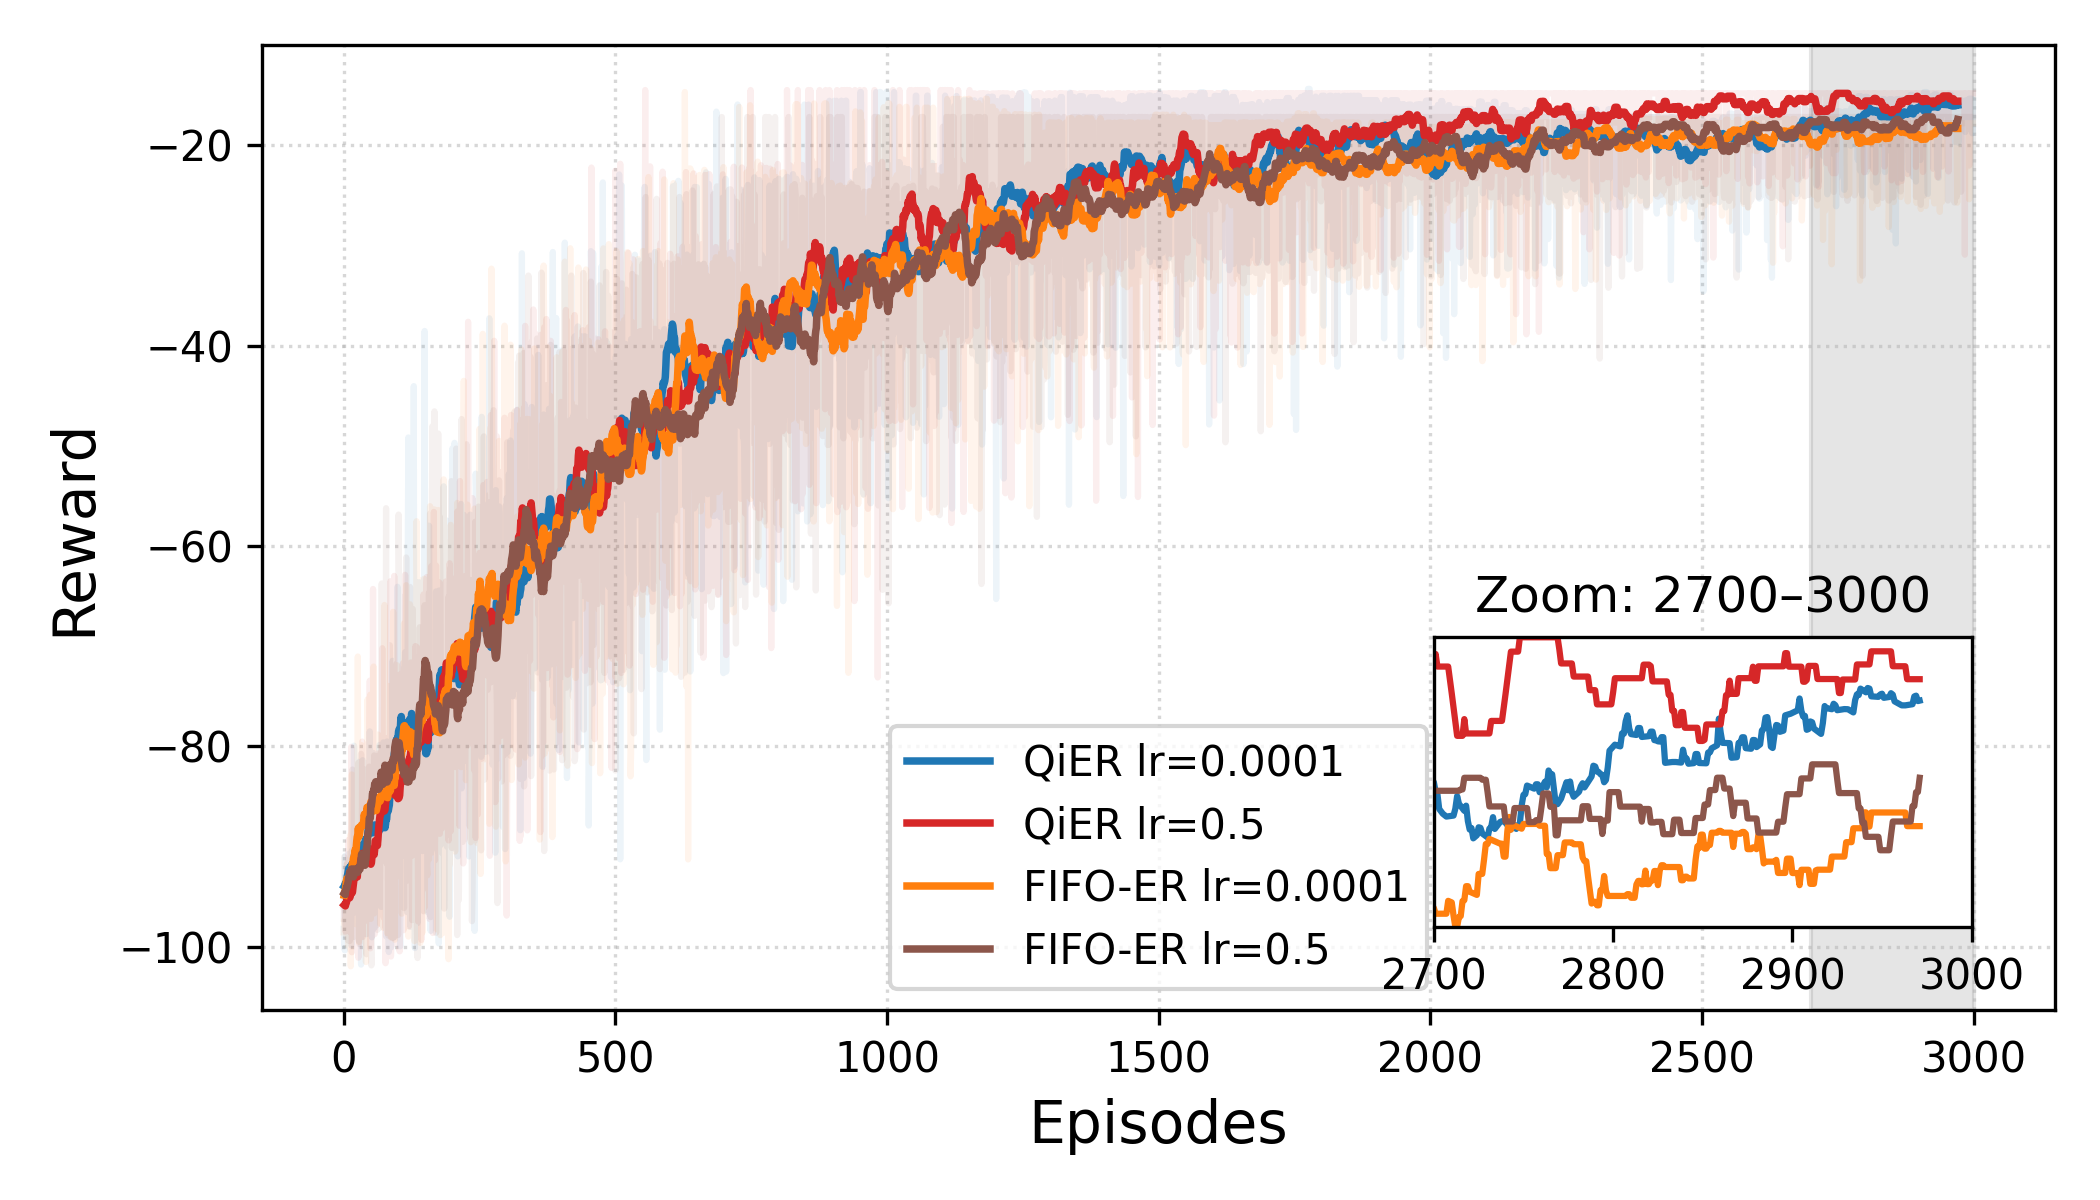
\includegraphics[width=\linewidth]{MinMax Cost Scaled/reward_with_inset_zoom.png}  % or any image name
    \caption{Rewards vs. episodes}
    \label{fig:reward_vs_episodes}
\end{figure}

Fig. \ref{fig:reward_vs_episodes} presents the reward across training episodes for various learning rates and model variants in the context of cache placement optimization at UAVs using binary decision variables. The proposed Heuristic-DDQN-QiER model with a learning rate of 0.5 demonstrates superior learning stability and maximum rewards, effectively optimizing the binary cache placement vector at each UAV. Also, H-DDQN-QiER variants with lower learning rate $0.0001$ perform equally well. However, the H-DDQN-FIFO-ER baseline with learning rates $0.0001$ and $0.5$ exhibit similar reward growth in the starting episodes but end up stabilising at lesser reward in the terminal phase as it can be seen in the zoomed part. This confirms the advantage of the QiER mechanism in enabling efficient and intelligent cache decisions in UAV-assisted networks over FIFO mechanism for Q-network learning.


% %---------------------------------------
% \begin{figure}[htbp]
%     \centering
%     \includegraphics[width=\linewidth]{regret_vs_episodes_with_noise_square.png}  % or any image name
%     \caption{System Regret vs Episodes}
%     \label{fig:System Regret vs Episodes}
% \end{figure}

% The fig. \ref{fig:System Regret vs Episodes} illustrates the convergence  behavior of {DDQN-QIER} and {DDQN-LRU} towards zero,  evaluated in terms of {system regret} $\mathcal{R}$ over learning episodes, where regret is defined as the difference between the maximum achievable cache hit ratio \( \mathcal{H}_{\text{max}} \) and the obtained $\mathcal{H}$ obtained by the agent for the overall system of UAVs.
% A lower system regret implies that the caching decisions are approaching optimality, thereby maximizing content availability i.e. the cache hit ratio  and minimizing latency. Both algorithms demonstrate declining regret with increasing episodes, indicating learning progression. Notably, DDQN-QiER achieves lower system regret and faster convergence due to its use of QiER, which helps in refining the caching policy more efficiently in dynamic request environments.
%---------------------------------------

\begin{figure}[htbp]
    \centering
    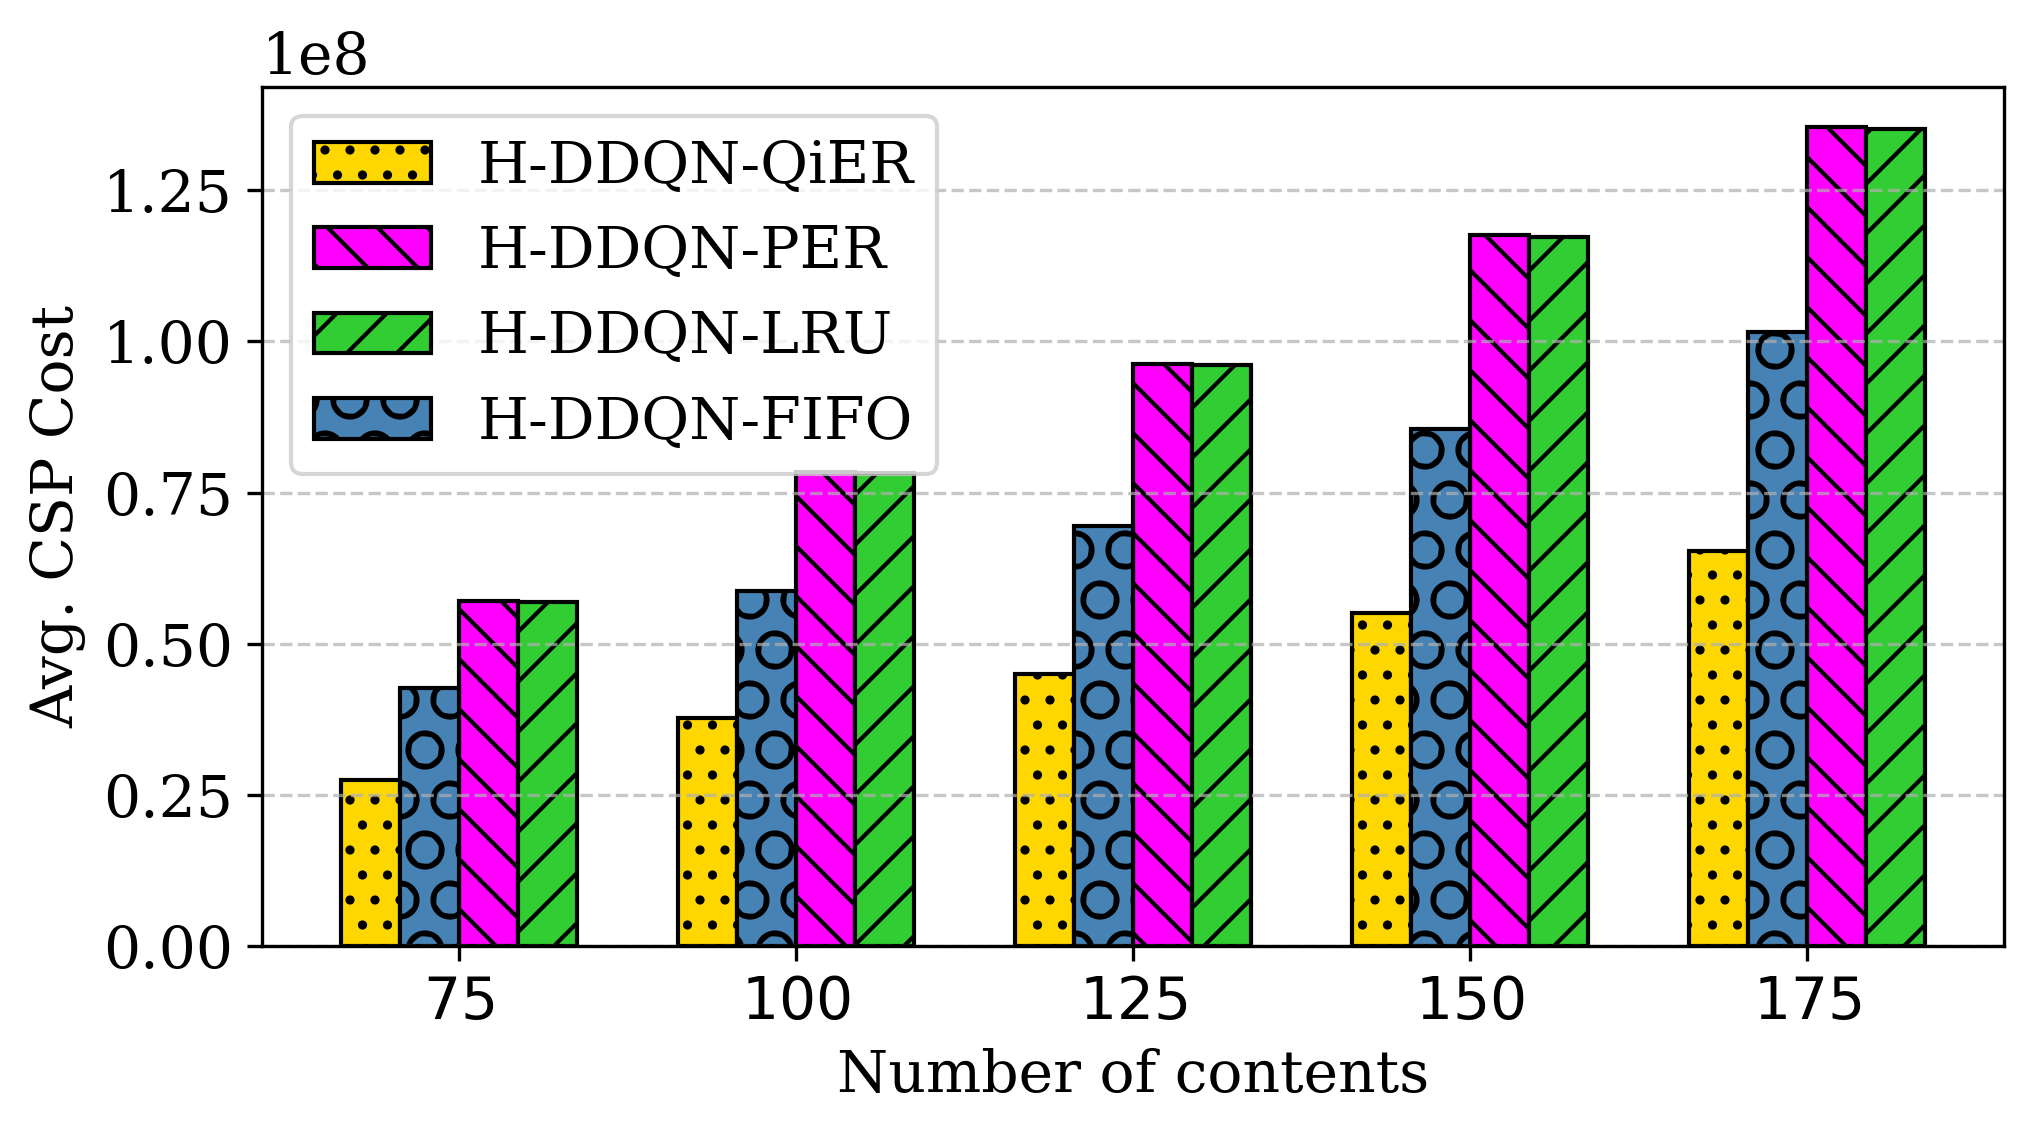
\includegraphics[width=\linewidth]{MinMax Cost Scaled/avg_cost_vs_files_bar.png}  % or any image name
    \caption{Average CSP cost vs no. of contents}
    \label{fig:avg_cost_vs_files}
\end{figure}
As shown in Fig. \ref{fig:avg_cost_vs_files}, the proposed H-DDQN-QiER mechanism consistently achieves the lowest average CSP cost across varying numbers of contents, outperforming all other variants. The trend supports the fact that when no. of contents are increased, the demand for those contents has come into play, but UAV had limited cache capacities leading to frequent cache misses and increasing the CSP cost. Despite this, QiER maintains a substantial cost advantage, demonstrating reductions of $\approx$ 52.3\% , 52.2\% and 35\% compared to PER, LRU and FIFO- ER, respectively. These results validate the efficiency and robustness of the QiER-based Q-network training approach in reducing CSP costs for UAV-enabled content caching frameworks.

%-----------------------------------
\begin{figure}[htbp]
    \centering
    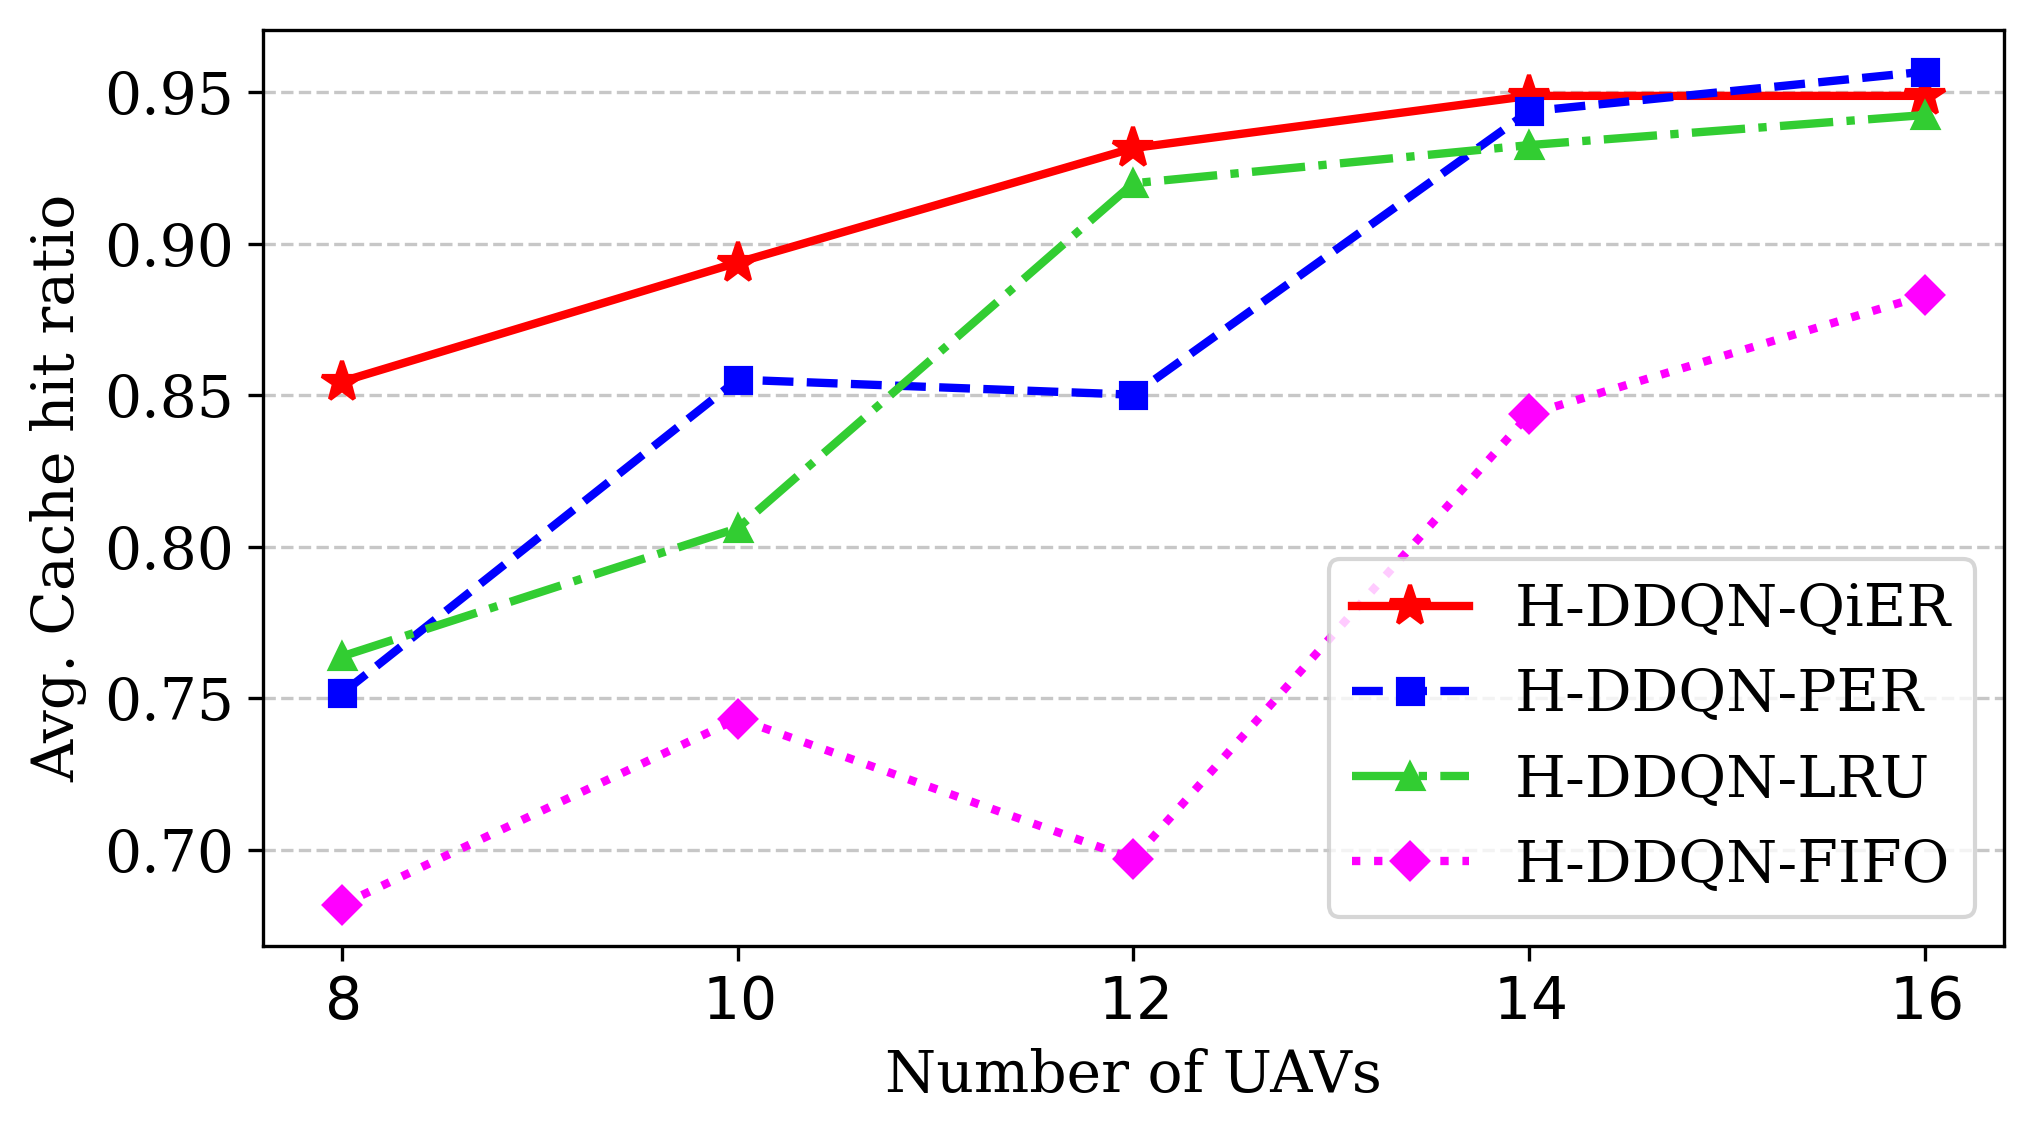
\includegraphics[width=\linewidth]{MinMax Cost Scaled/avg_CHR_vs_uavs_linegraph.png}  % or any image name
    \caption{Avg cache hit ratio vs. UAVs}
    \label{fig:avg_chr_vs_uav}
\end{figure}
As shown in Fig.~\ref{fig:avg_chr_vs_uav}, H-DDQN-QiER achieves the highest average cache hit ratio across all UAV counts, consistently outperforming all other variants. The trend is seen in the way that, as the number of UAVs increase~($\uparrow$), the cache hit ratio increases~($\uparrow$), because more UAVs in a cluster increase the chance of cluster-assisted content delivery, hence reducing CSP cost for retrieving the same content from backhaul links from CSP via satellite. Specifically, H-DDQN-QiER achieves a $5.5\%$ and $5.2\%$ higher cache hit ratio than H-DDQN-PER and H-DDQN-LRU, respectively, and a significant $19.8\%$ improvement over H-DDQN-FIFO. This is evident from Fig.~\ref{fig:avg_cost_vs_uavs}. In addition, the system regret, which is essentially the cache miss, should decrease~($\downarrow$). This is also validated by Fig.~\ref{fig:avg_system_regret_vs_uavs} that increasing UAVs reduces system regret.


\begin{figure}[htbp]
    \centering
    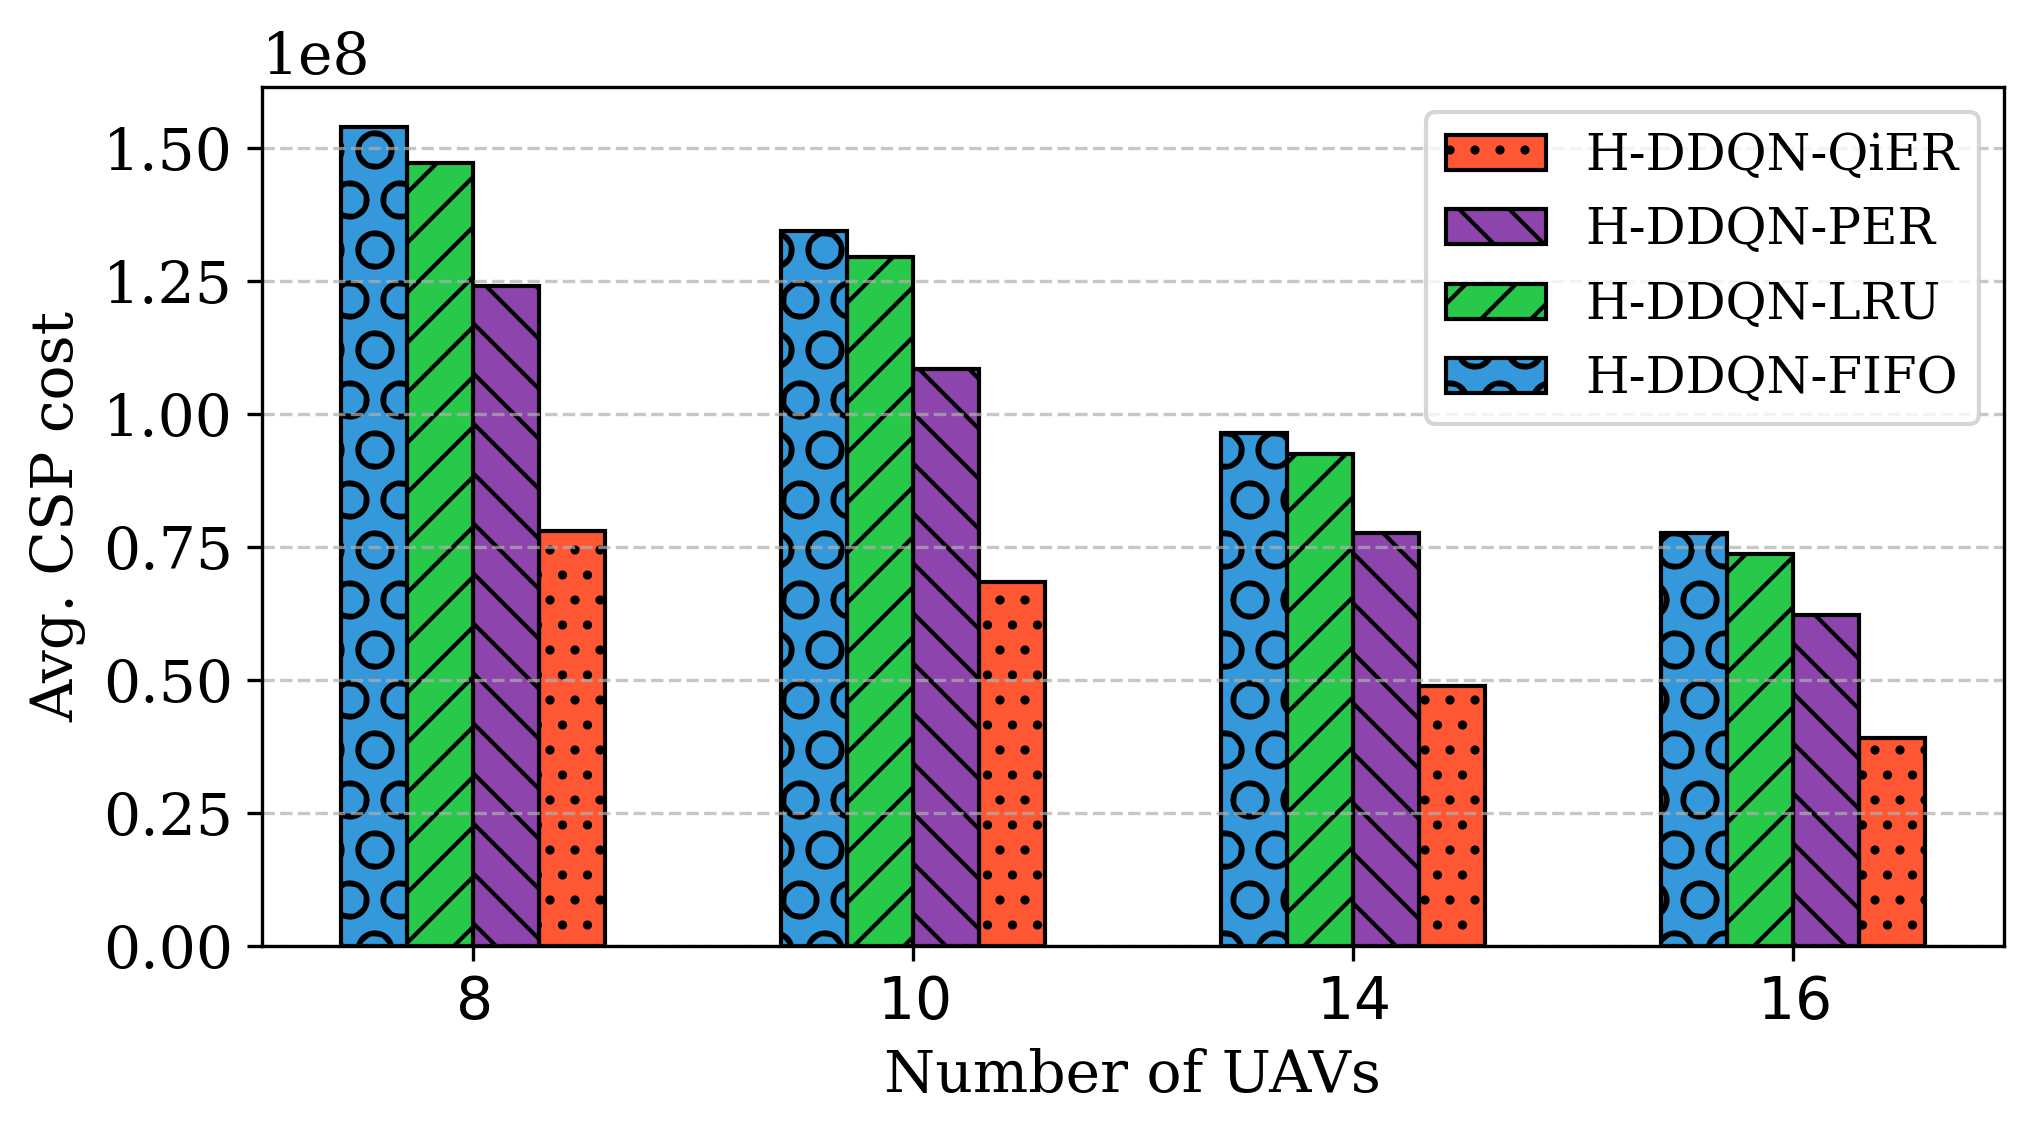
\includegraphics[width=\linewidth]{MinMax Cost Scaled/avg_cost_vs_uavs_bar.png}  % or any image name
    \caption{Avg. CSP cost vs No. of UAVs}
    \label{fig:avg_cost_vs_uavs}
\end{figure}
%------------------------------------
%--------------------------------
\begin{figure}[htbp]
    \centering
    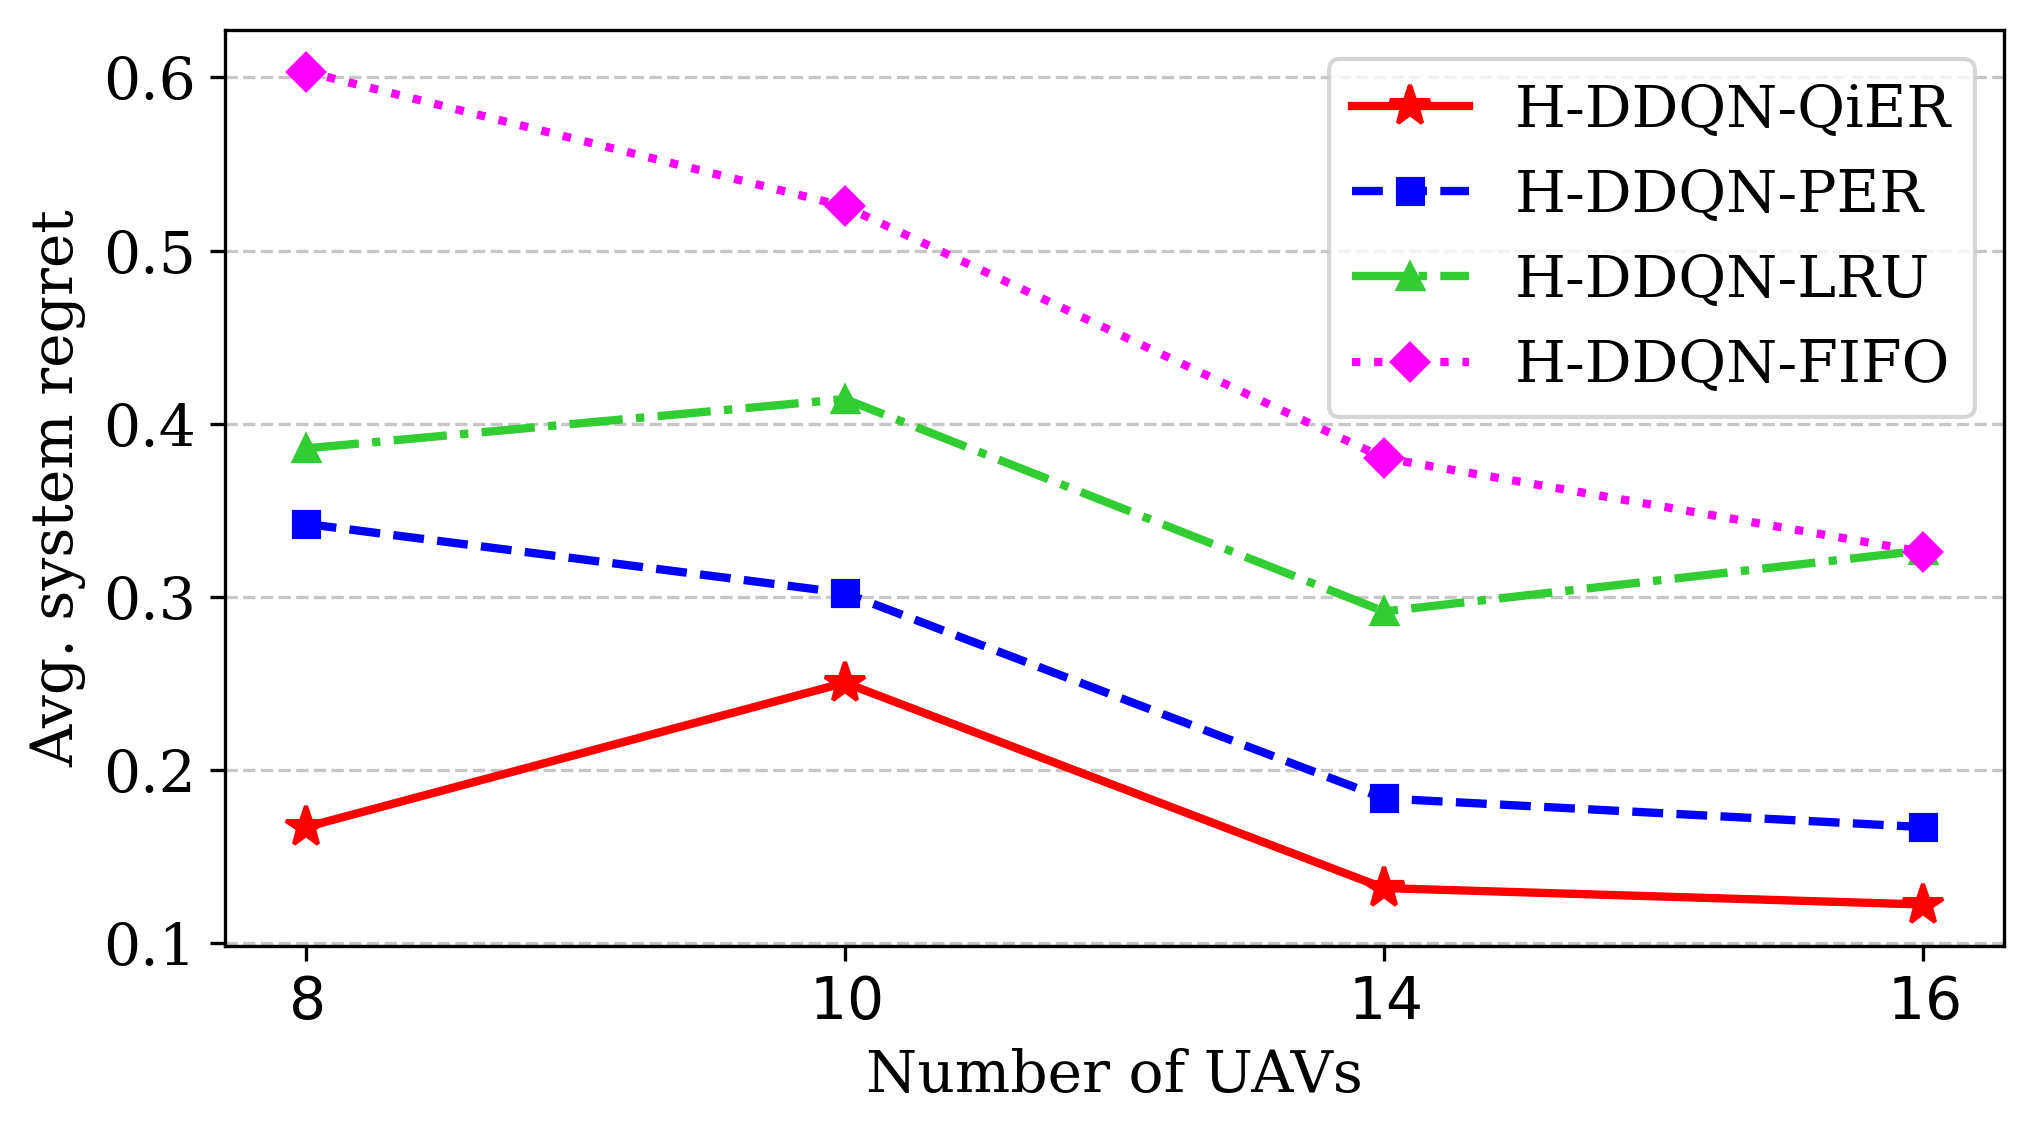
\includegraphics[width=\linewidth]{MinMax Cost Scaled/avg_Systemregret_vs_uavs_line.png}  % or any image name
    \caption{Avg. System regret vs. No. of UAVs}
    \label{fig:avg_system_regret_vs_uavs}
\end{figure}


%---------------------------------------
Fig. \ref{fig:avg_COST_vs_transmission_capacity} shows that the average CSP cost decreases as the transmission capacity increases. This is because transmission capacity determines the maximum number of files a UAV can retrieve from the CSP upon a cache miss. A higher transmission capacity says that more no. of contents can be retrieved from CSP to accomodate in cache vector of a UAV, reducing the number of cache misses, which previously required costly CSP access. Among the models, H-DDQN-QiER consistently achieves lower CSP cost, especially at higher value, due to its efficient cache replacement strategy that reduces dependency on CSP content retrieval.
\begin{figure}[htbp]
    \centering
    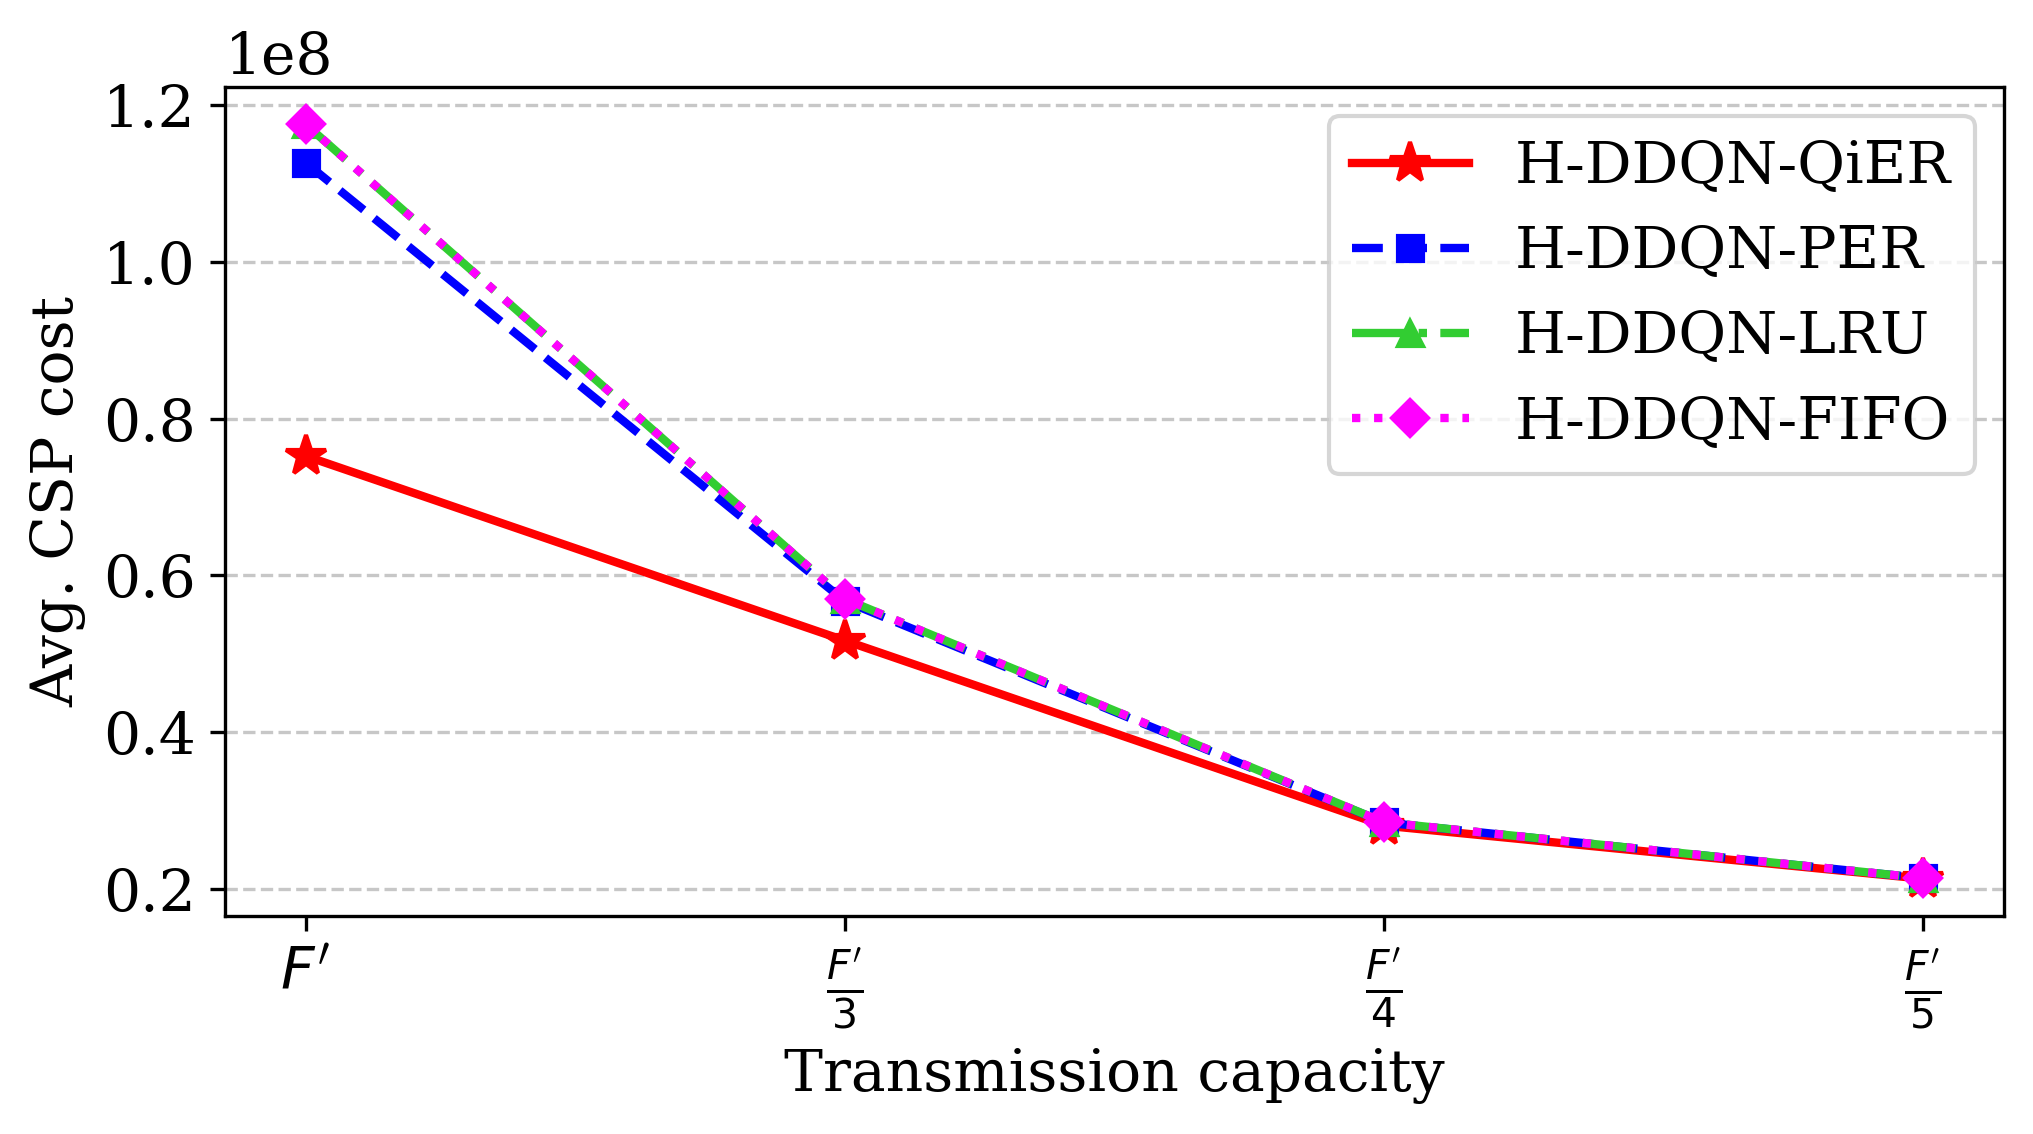
\includegraphics[width=\linewidth]{MinMax Cost Scaled/avg_COST_vs_transmission_capacity.png}  % or any image name
    \caption{Avg. CSP cost vs Transmission Capacity}
    \label{fig:avg_COST_vs_transmission_capacity}
\end{figure}

% %---------------------------------------
% \begin{figure}[htbp]
%     \centering
%     \includegraphics[width=\linewidth]{cost_vs_episodes_learning_Rate.png}  % or any image name
%     \caption{Cost for content retrieval from CSP via satellite vs. episodes}
%     \label{fig:cost_vs_episodes_learning}
% \end{figure}
% In fig. \ref{fig:cost_vs_episodes_learning}, the proposed DDQN-QiER model demonstrates a superior cost-efficiency in retrieving content from the CSP via satellite during the initial training phase, as shown in the zoomed inset (Episodes 0–50). Compared to other variants, including DDQN-LRU and DDQN-QiER with different learning rates, our model exhibits a significantly lower retrieval cost early in training. As training progresses, all models converge toward a similar cost level, indicating stability and learning saturation. However, the initial performance advantage of DDQN-QiER highlights its effectiveness in rapidly minimizing retrieval cost, which is critical in real-time, resource-constrained environments.

%---------------------------------------
Fig \ref{fig:avg_chr_vs_users} shows that the average cache hit ratio varies slightly with the number of users, but H-DDQN-QiER consistently achieves the highest hit ratio when compared to other three variants. The variation is due to the fact that when no. of users increases, the request for diverse content also increases, but since UAV has a limited cache capacity and can cache some contents only,  leading to cache miss for remaining uncached contents.
\begin{figure}[htbp]
    \centering
    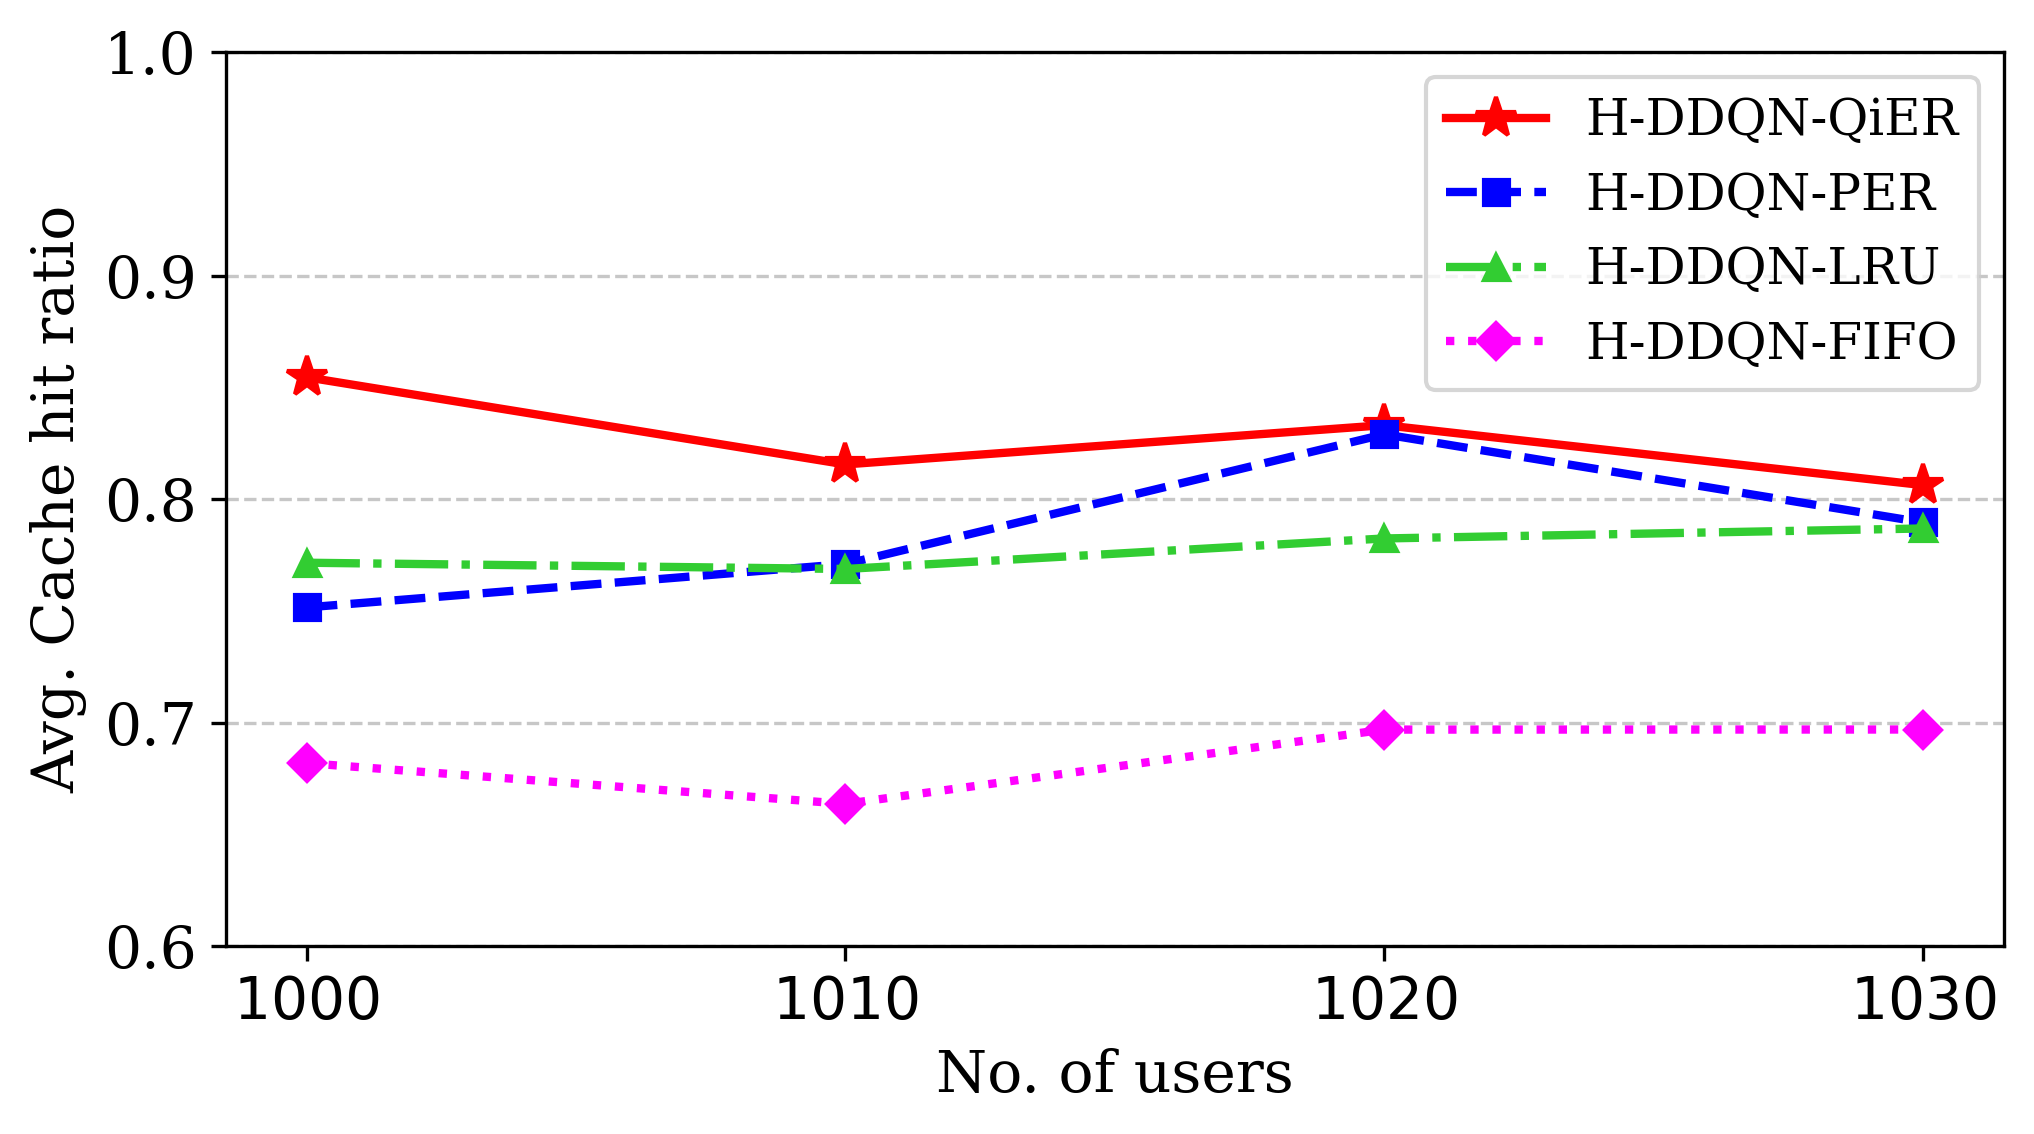
\includegraphics[width=\linewidth]{MinMax Cost Scaled/avg_chr_vs_users_line.png}  % or any image name
    \caption{Cache Hit Ratio vs. Users}
    \label{fig:avg_chr_vs_users}
\end{figure}


%---------------------------------------
Fig. \ref{fig:avg_chr_vs_cache_capacity} illusatrated the comparison of cache hit ratio for different cache capacity of UAVs with different variant replay buffer of H-DDQN. It is clearly evident that the proposed H-DDQN-QiER outperforms all other variants. The trend is supported by the fact that, when cache capacity of a UAV increases $\uparrow$ , it can accomodate more no of. contents in its cache vector, leading to less system regret (i.e. higher cache hit or equivalently lesser cache miss) and the lowers the CSP retrieval cost. This explanation is also supported by fig. \ref{fig:avg_chr_vs_cache_capacity}, fig. \ref{fig:avg_cost_vs_cache_capacity} and fig. \ref{fig:avg_system_regret_vs_cache_capacity}.
\begin{figure}[htbp]
    \centering
    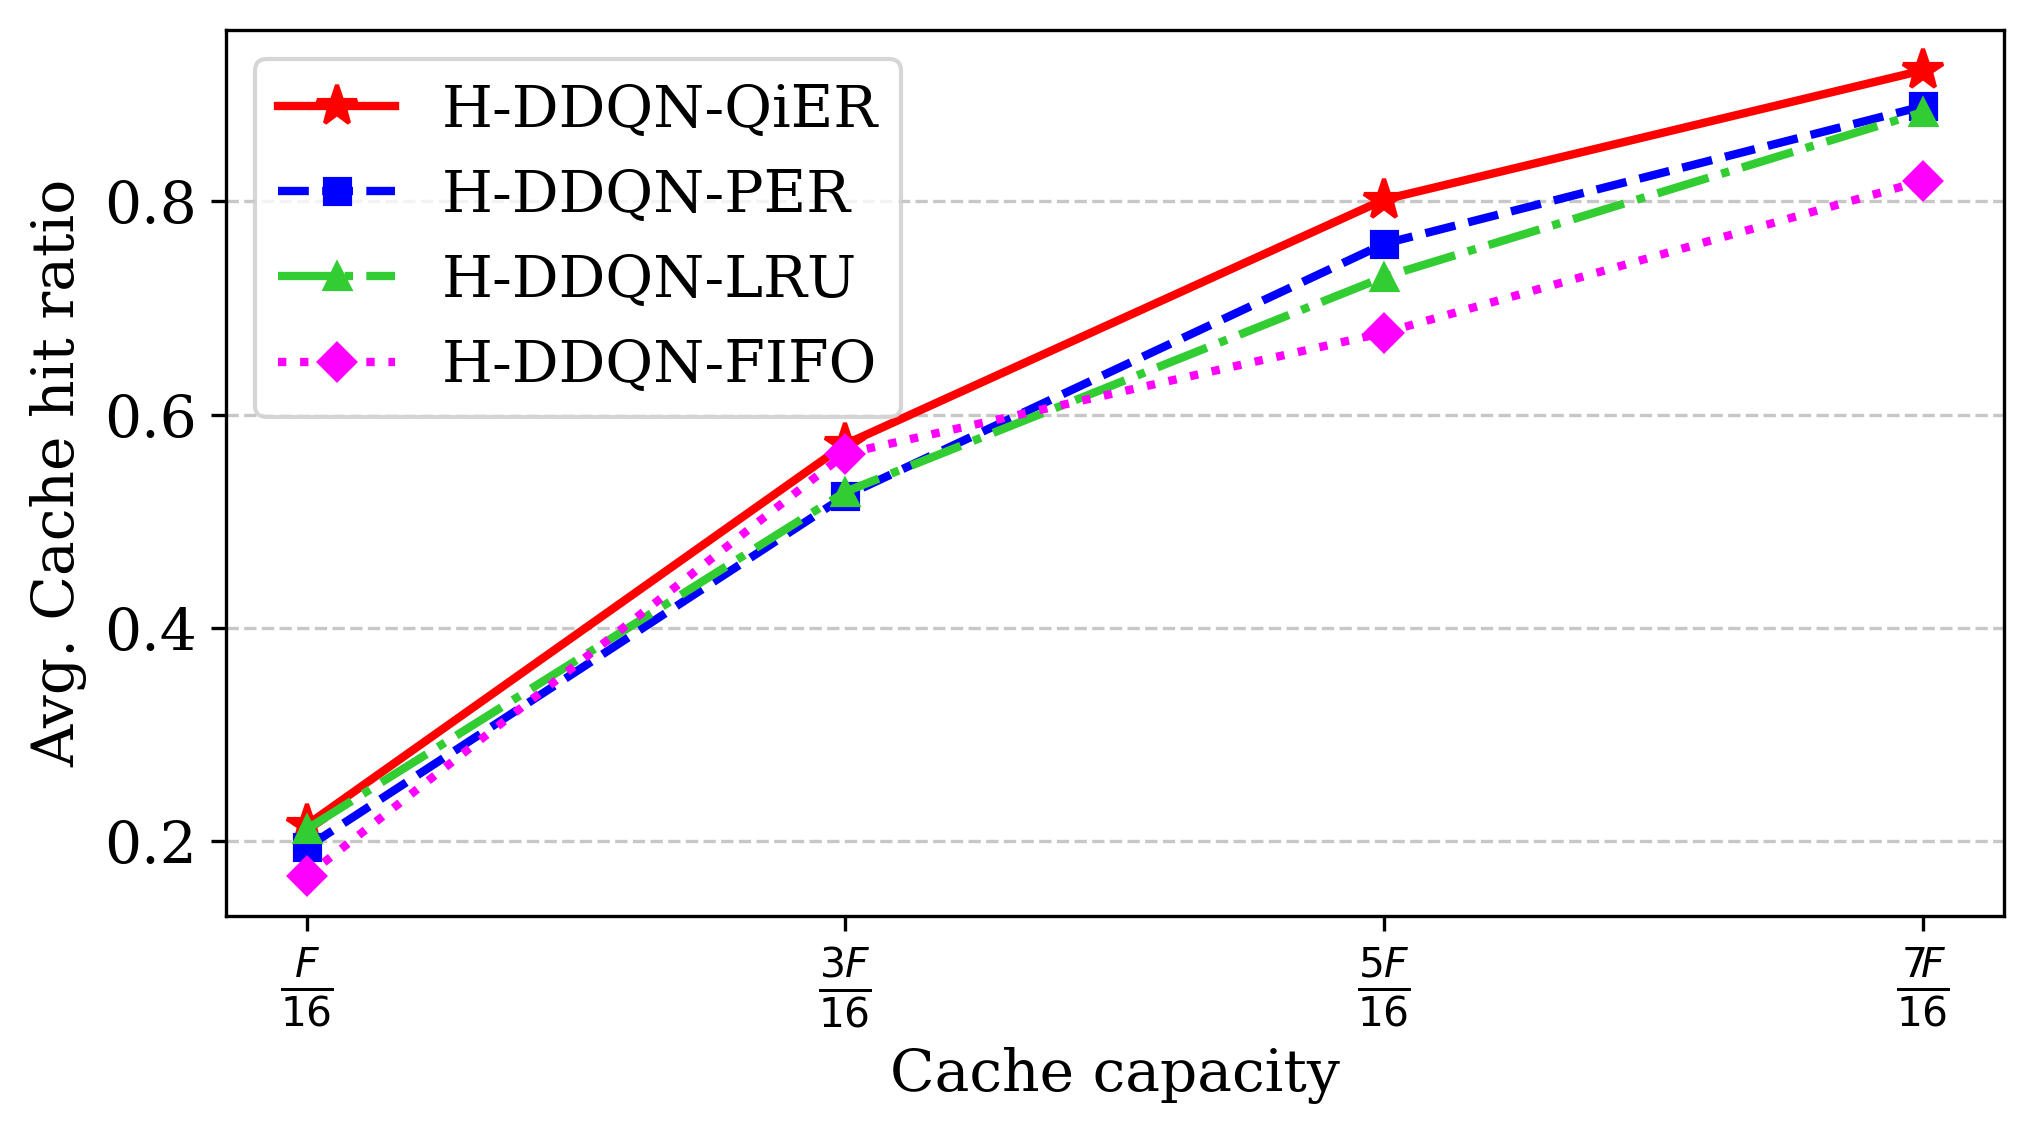
\includegraphics[width=\linewidth]{MinMax Cost Scaled/avg_chr_vs_capacity_linegraph.png}  % or any image name
    \caption{Avg. Cache hit ratio vs. Cache capacity}
    \label{fig:avg_chr_vs_cache_capacity}
\end{figure}

%---------------------------------------

% \begin{figure}[htbp]
%     \centering
%     \includegraphics[width=\linewidth]{uavs_chr.png}  % or any image name
%     \caption{Cache Hit Ratio vs. UAVs}
%     \label{fig:uavs_chr}
% \end{figure}
% %---------------------------------------


% \begin{figure}[htbp]
%     \centering
%     \includegraphics[width=\linewidth]{users_chr.png}  % or any image name
%     \caption{Cache Hit Ratio vs. Users}
%     \label{fig:users_chr}
% \end{figure}

% As shown in Fig. \ref{fig:users_chr}, the proposed H-DDQN-QiER demonstrates superior performance compared to both H-DDQN-PER and H-DDQN-LRU in achieving a higher average cache hit ratio as the number of users varies. At 1000 users, QiER attains a cache hit ratio of approximately 0.57, while PER and LRU achieve ratios of 0.447 and 0.324, respectively, showcasing improvements of approximately 27.5\% over PER and 76\% over LRU. At 1040 users, QiER maintains a cache hit ratio of about 0.62, compared to 0.454 for PER and 0.324 for LRU, representing enhancements of roughly 36.5\% and 91.4\%, respectively.
% Throughout the range of user counts, QiER consistently performs better, with its hit ratio improving slightly as the number of users increases, peaking at approximately 0.63 around 1020–1030 users. Conversely, PER and LRU show relatively stagnant or fluctuating trends, with PER peaking around 0.475 and LRU remaining steady at approximately 0.324.
% These results highlight the robustness and adaptability of H-DDQN-QiER, making it well-suited for scalable caching frameworks in dynamic user environments. In contrast, PER and LRU exhibit limitations in effectively managing cache hits as user numbers increase.
%---------------------------------------

% As shown in Fig. \ref{fig:avg_COST_vs_transmission_capacity} the proposed H-DDQN-QiER consistently outperforms both H-DDQN-PER and H-DDQN-LRU in maximizing the average cache hit ratio across varying numbers of users. At 1000 users, QiER achieves a cache hit ratio of approximately 0.57, compared to 0.447 (PER) and 0.324 (LRU), reflecting improvements of approximately 27.5\% and 76\%, respectively. Similarly, at 1040 users, QiER maintains a higher cache hit ratio of approximately 0.62, compared to 0.454 (PER) and 0.324 (LRU), representing improvements of around 36.5\% and 91.4\%, respectively.

% This consistent performance demonstrates the superiority of QiER in leveraging its experience replay mechanism to enhance caching efficiency. In contrast, PER and LRU show relatively modest improvements with increasing user numbers, indicating their limited scalability. The results confirm the effectiveness of H-DDQN-QiER for proactive caching in user-intensive scenarios, highlighting its potential for optimizing cache utilization in dynamic environments.
%---------------------------------------

%---------------------------------------


% As shown in Fig. \ref{fig:avg_chr_vs_uavs_bar}, the average cache hit ratio improves with increasing UAVs for all methods, confirming the scalability of our cluster-based caching. A cache hit is counted if any UAV in the cluster stores the requested content, so adding UAVs (from 8 to 16) enhances content availability. DDQN-QiER initially performs lower ( $\mathcal{H}_{avg} \approx$ 0.53) due to the approximations in the classical simulation of quantum memory. However, it quickly catches up, surpasses DDQN-LRU, and matches DDQN-PER. QiER effectively prioritizes important experiences using TD-error-based quantum-inspired weights, offering a scalable and intelligent caching framework with efficient learning performance.

%---------------------------------------

\begin{figure}[htbp]
    \centering
    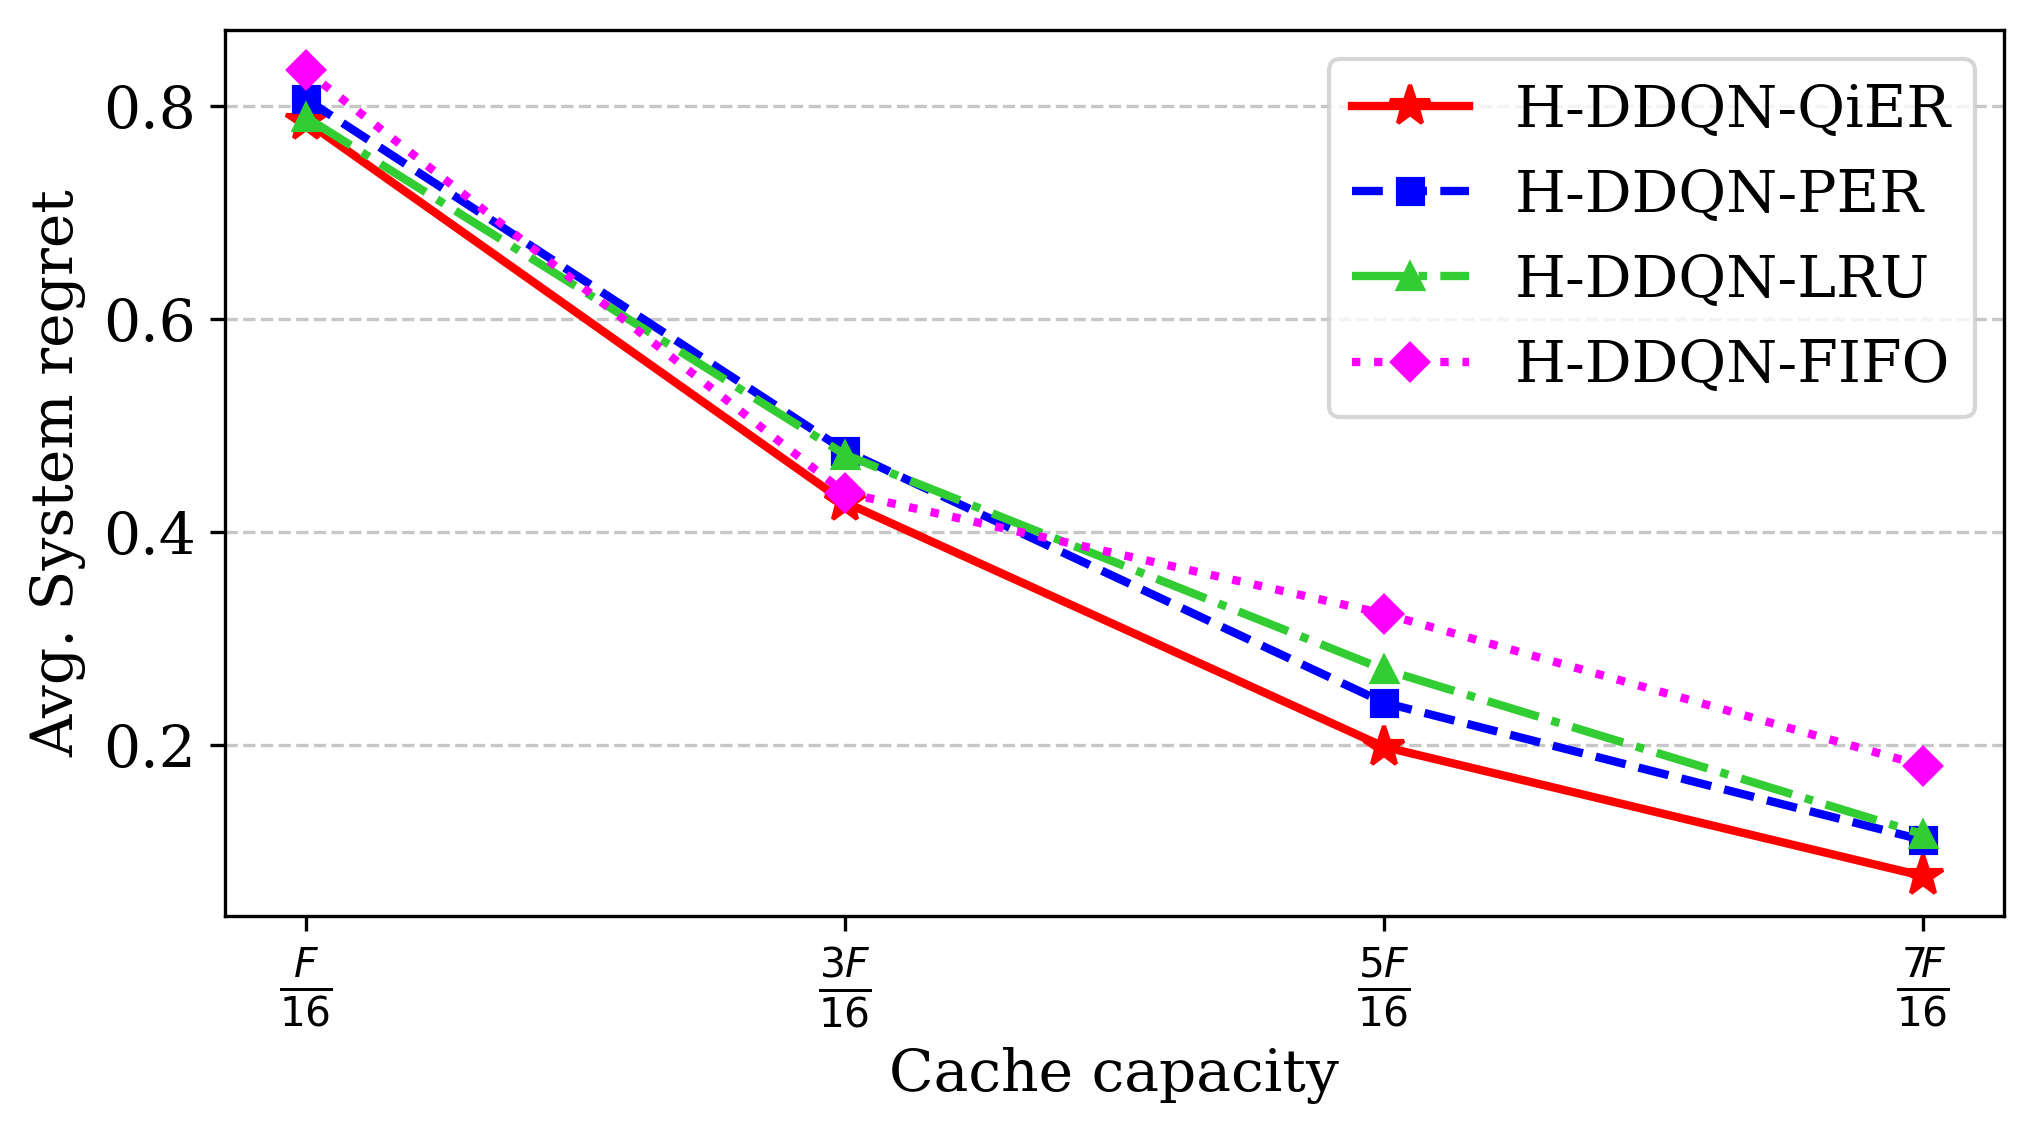
\includegraphics[width=\linewidth]{MinMax Cost Scaled/IEEE_avg_COST_vs_cache_capacity_lineplot.png}  % or any image name
    \caption{Avg. System regret vs. Cache capacity}
    \label{fig:avg_system_regret_vs_cache_capacity}
\end{figure}

%---------------------------------------

\begin{figure}[htbp]
    \centering
    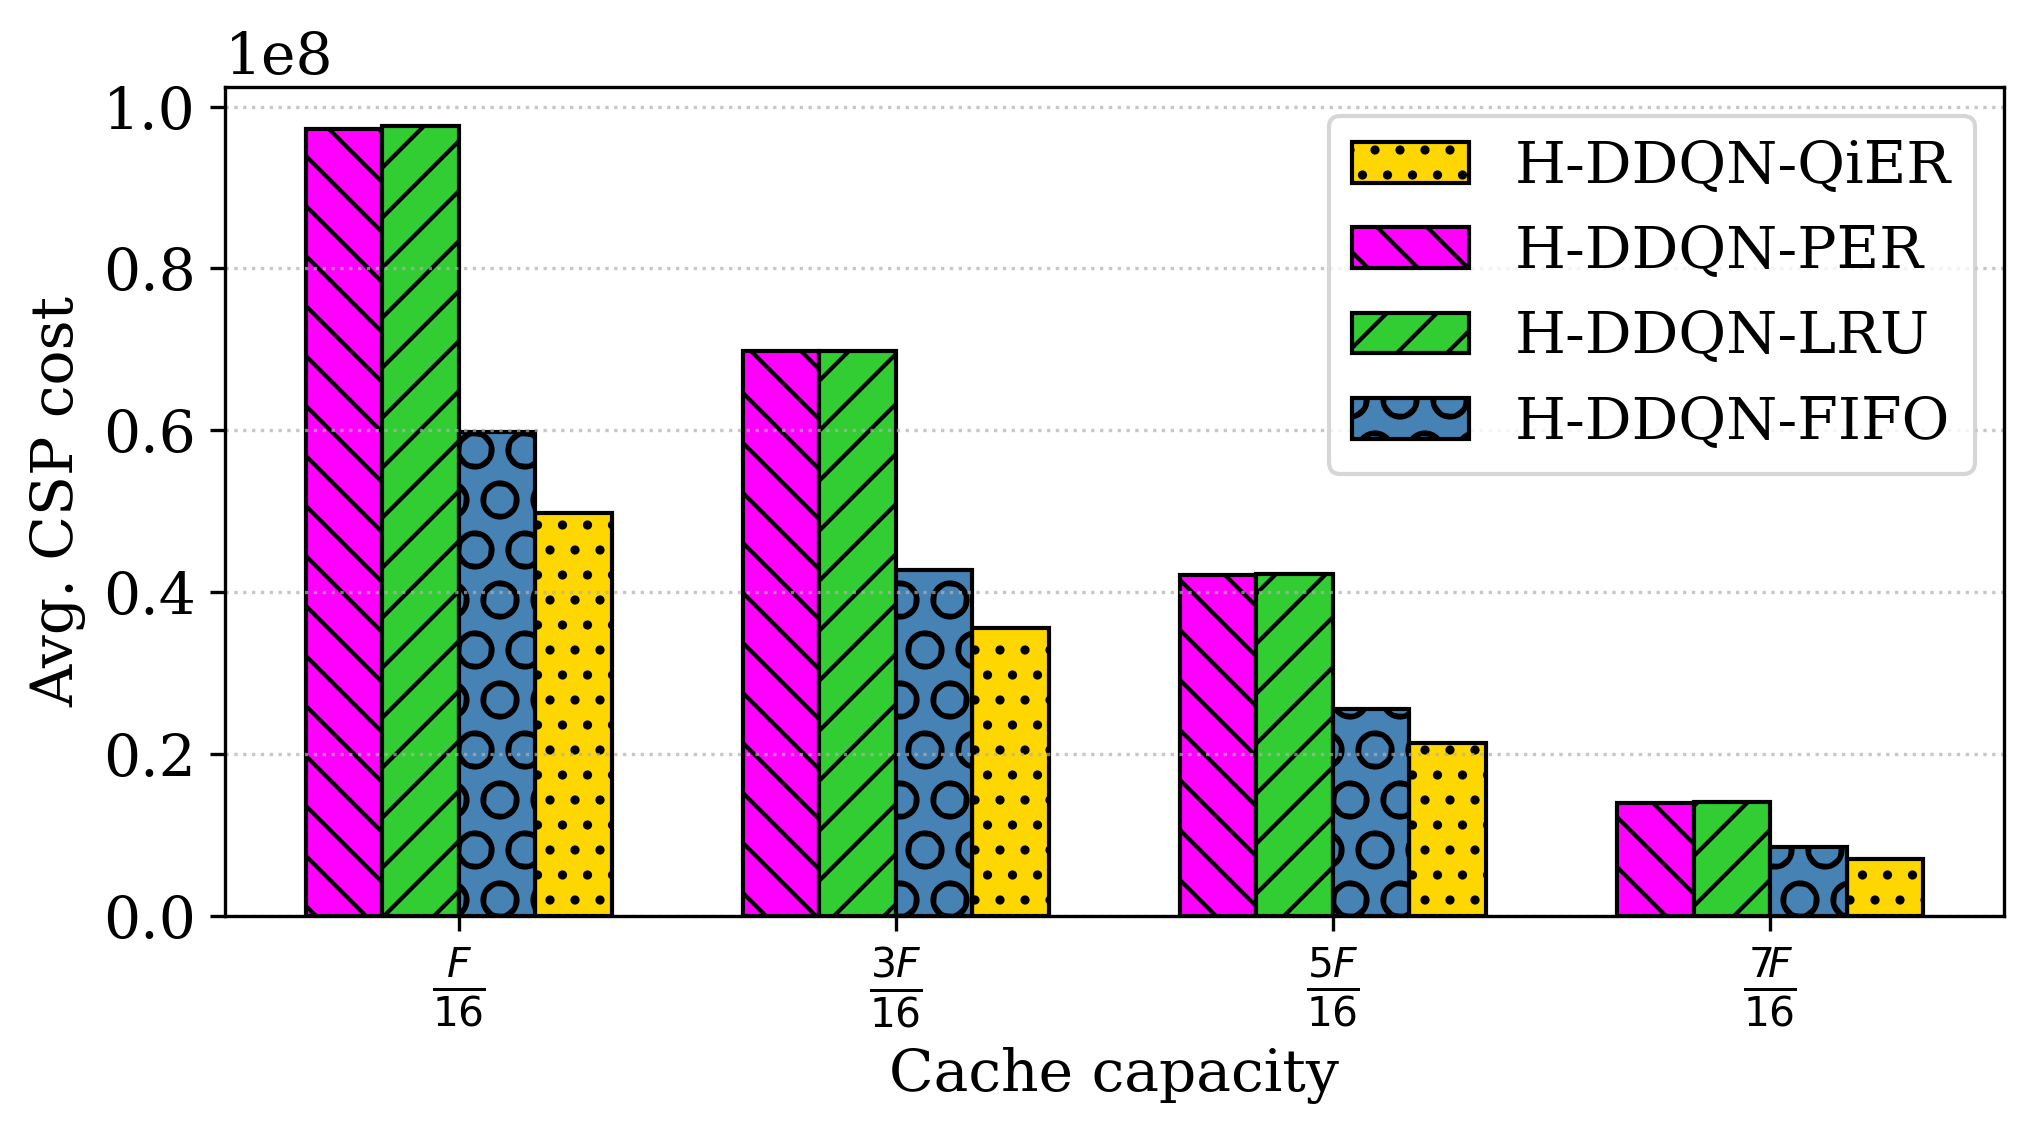
\includegraphics[width=\linewidth]{MinMax Cost Scaled/avg_cost_vs_cache_capacity_bar.png}  % or any image name
    \caption{Avg. Cost for content retrieval from CSP via satellite vs. Cache capacity}
    \label{fig:avg_cost_vs_cache_capacity}
\end{figure}
% Fig. \ref{fig:avg_cost_vs_cache_capacity} illustrates the average cost incurred for CSP by QiER, FIFO, and PER strategies in model training under varying cache capacities. QiER consistently achieves the lowest CSP cost due to its efficient Q-network learning driven. In contrast, FIFO and PER experiences challenge in training Q-network leading to bad cache decisions. Consequently, UAVs relying on these strategies face more cache misses and are forced to retrieve content from the CSP more frequently, increasing the overall retrieval cost. It is observed that when cache capacity increases, the CSP cost deacreses due to that fact that now UAV can cache more files, leading to less cache miss. Hence, the system regret which is equivalent to cache miss also decreases with increasing cache capacity, which is evident from from fig. \ref{fig:avg_system_regret_vs_cache_capacity}. 
% In addition, the fig. \ref{fig:avg_chr_vs_cache_capacity} verifies that the cache hit ratio also should increase with increasing cache capacity. 

%-----------------------------

% Fig. \ref{fig:avg_chr_vs_cache_capacity} compares the average cache hit ratio of QiER (proposed) framework with FIFO-ER, PER, and Random-caching strategies across varying UAV cache capacities. It can be seen that all three types of replay buffer has almost similar performance but specifically LRU based buffer gives slighty lesser CHR in comparison other two. However, Random-Caching strategy performs the worst owing to its lack of content relevance awareness. The CHR improves with larger cache sizes ($e.g.$, 7/16F), as each UAV can store more popular files, enhancing cooperative file availability within the cluster



%---------------------------------------



%---------------------------------------
\section{Conclusion and Upcoming Projects}
In this work, we considered a UAV-satellite-assisted edge caching scenario and proposed a proactive data caching approach using a heuristic-based modified Deep Double Q-Network with quantum inspired experience replay (Heuristic-DDQN-QiER). We jointly minimize the system regret and the CSP cost to maximize the UAV cache ratio. Numerous experiments are built using real-world datasets, such as Movielens, and the outcomes confirm the effectiveness of the and the suggested method's advantages over a number of other methods.

For upcoming projects, we plan to prolong the current model by incorporating dynamic user mobility and adaptive UAV association to better reflect real-world scenarios. Furthermore, integrating moving satellites and enabling inter-satellite communication would support cooperative caching and broader content distribution. The application of SDN could provide centralized control and optimization over the caching process.

\bibliographystyle{ieeetr}
\bibliography{IEEEfull}


\end{document}
